\documentclass[twoside]{mitthesis}
% \usepackage{listings}
\usepackage{xcolor} % Para colores
\usepackage{minted}
% \usepackage{hyperref}
\usepackage[spanish]{babel}
\usepackage{amsmath,amssymb,amsfonts}		
\usepackage{booktabs}
\usepackage{array}
\usepackage{pdfpages}
\usepackage{graphicx}

\usepackage{tikz}
\usetikzlibrary{shapes.geometric, arrows.meta, positioning}

\tikzstyle{etapa} = [rectangle, rounded corners, minimum width=8cm, minimum height=1cm,text centered, draw=black, font=\small, text=black]
\tikzstyle{orangebox} = [etapa, fill=orange!70]
\tikzstyle{yellowbox} = [etapa, fill=yellow!70]
\tikzstyle{cyanbox} = [etapa, fill=cyan!40]
\tikzstyle{arrow} = [thick,->,>=stealth]




% \definecolor{dartkeyword}{rgb}{0.13,0.13,0.81}
% \definecolor{dartcomment}{rgb}{0.56,0.35,0.01}

% \lstdefinelanguage{dartstyle}{
%     keywords={async, await, break, case, catch, class, const, continue, default, do, else, enum, export, extends, factory, false, final, finally, for, if, in, is, new, null, required, return, super, switch, this, throw, true, try, var, void, while, with},
%     sensitive=true,
%     comment=[l]{//},
%     morecomment=[s]{/*}{*/},
%     string=[b]",
%     morestring=[b]',
%     morestring=[b]'''
% }


\usemintedstyle{vs} 






% %%%%%%%%%%%%%%%%%%%%%%%%%%%%%%%%%%%%%%
\newtheorem{notation}{Notación}[chapter]
\newtheorem{theorem}{Teorema}[chapter]
\newtheorem{definition}{Definición}[chapter]
\newtheorem{lemma}{Lema}[chapter]
%% Set chemical formulas nicely
% \usepackage[version=4]{mhchem}%   documentation is here https://ctan.org/pkg/mhchem
\graphicspath{{assets/}}
\usepackage{csquotes} 

\usepackage[
    style=apa,
    sortcites=true,
    sorting=nyt,
    backend=biber,
    language=spanish,
    hyperref=true,
    backref=true,
]{biblatex}

\addbibresource{bibliography.bib}

\hypersetup{
	pdfsubject={Ecuaciones de Navier-Stokes},
	pdfkeywords={Universidad Autónoma Chapingo, UACh},
	pdfurl={},
	pdfcontactemail={emilioah02@gmail.com},
	pdfauthortitle={Ing.}
}

\pagestyle{plain}

\def\all{all}
\ifx\files\all \typeout{Including all files.} \else %\typeout{Including only \files.} \includeonly{\files} \fi

% Márgenes
\geometry{left=4cm, right=2.5cm, top=5cm, bottom=2.5cm}


\begin{document}
%%%%%%% 1. PORTADA Y FIRMAS %%%%%%%
\includepdf[pages=1]{0cover.pdf}
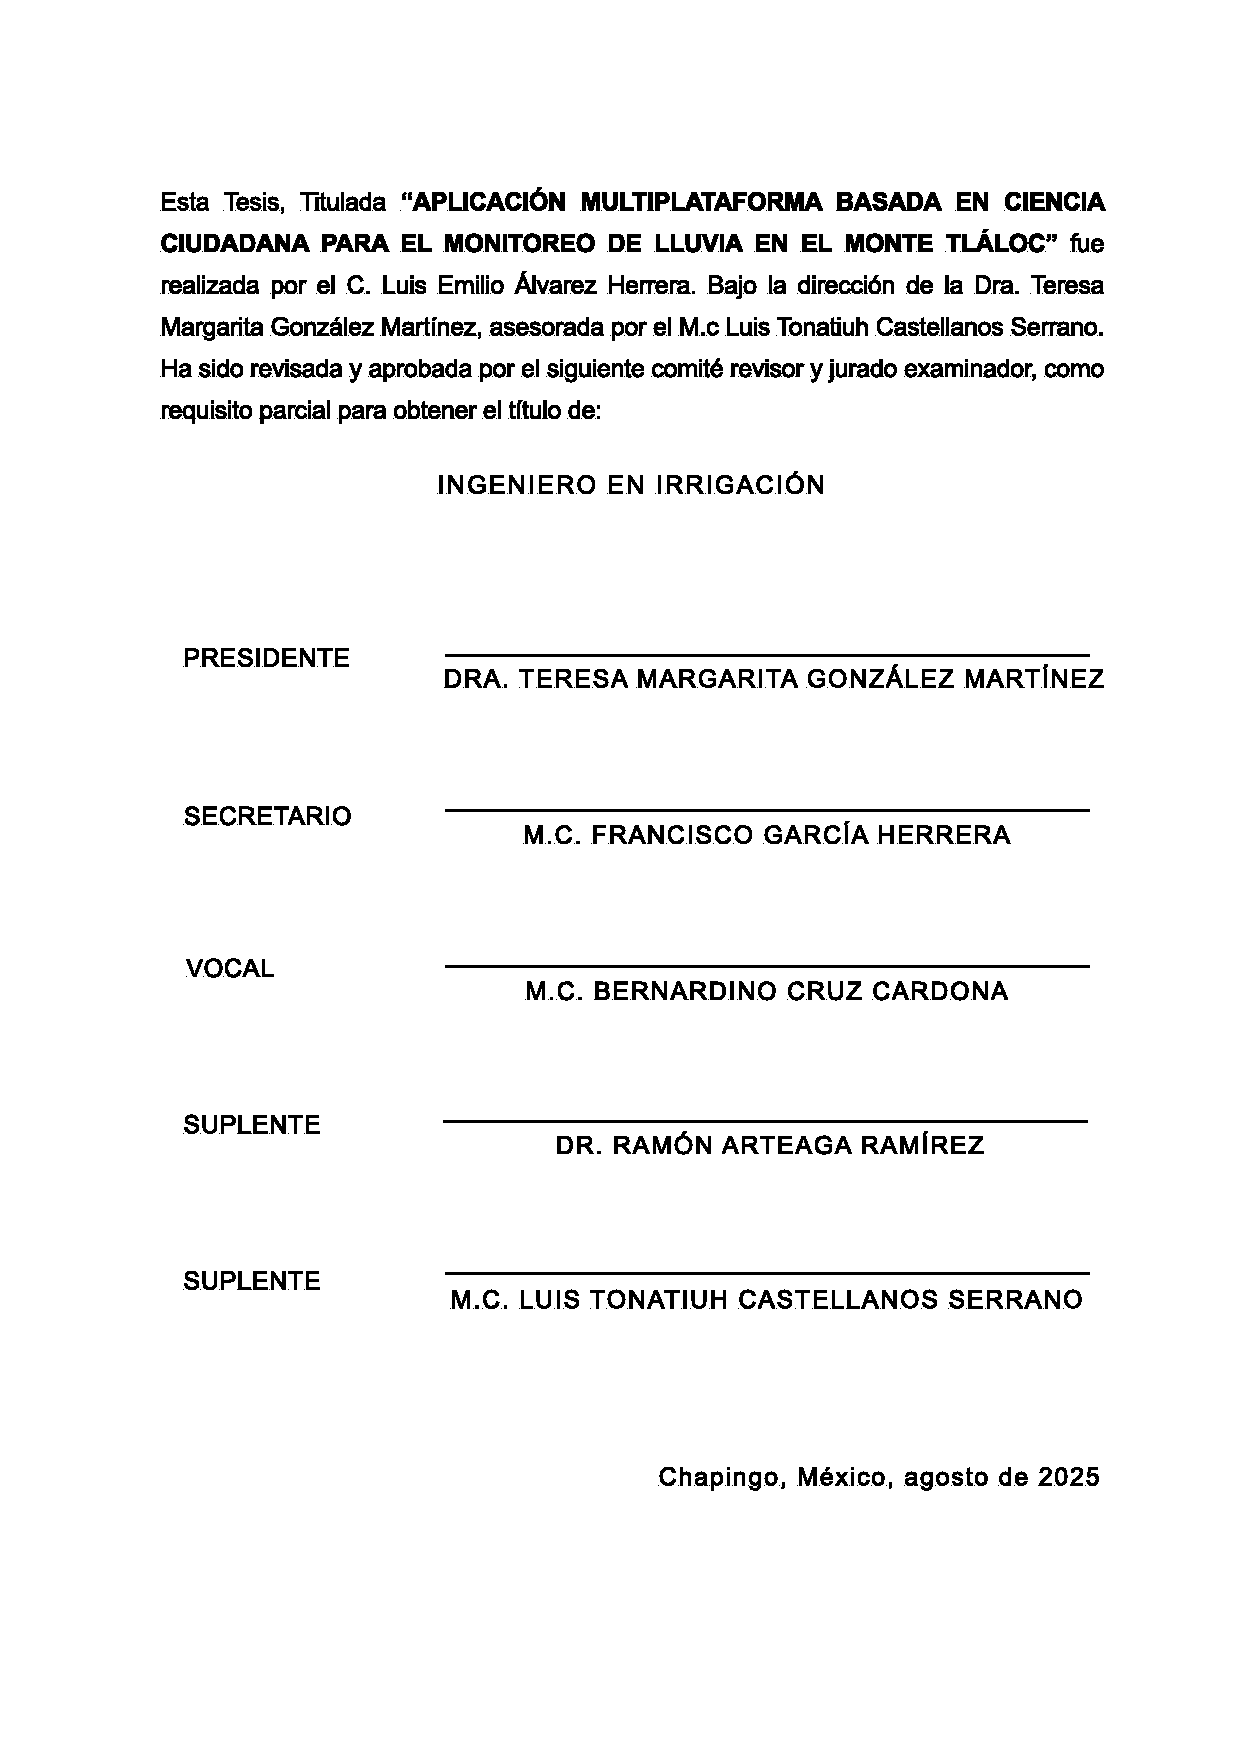
\includepdf[pages=1]{01sign.pdf}
%%%%%%% INICIA NÚMEROS ROMANOS %%%%%%%
\pagenumbering{roman}


\chapter*{AGRADECIMIENTOS}
\addcontentsline{toc}{chapter}{AGRADECIMIENTOS}
\begin{center}
    \texttt{``La educación agrícola es la base para una nación fuerte y autosuficiente''} - Marte R. Gómez, padre de la Universidad Autónoma Chapingo, ingeniero hidráulico hoy de irrigación.
\end{center}

Hago especial reconocimiento por las enseñanzas y valores que adquirí gracias a la \textbf{Universidad Autónoma Chapingo}: por ofrecerme la beca institucional, por la beca PROFONI referente a la investigación; por la beca SUBES y Benito Juarez del gobierno de México; al Comedor Central y Unidad Médica por su servicio de primera calidad; en especial estoy agradecido a causa de toda la inversión por concepto de:
\begin{itemize}
    \item Congreso Internacional en Santiago Chile, \item Intercambio Académico Internacional que fue en la Universidad de Agricultura de Tokio, 
    \item por la estancia pre-profesional en EcosueloLab Chile, 
    \item Viajes de estudio en México
    \item y por sus numerosos vínculos con instituciones prestigiosas, especialmente con el Colegio de Posgraduados de donde surgió este trabajo.
\end{itemize}

Hago un distinguido reconocimiento a las y los maestros que me han enseñaron desde el kinder hasta la universidad, todos ellos merecen nuestro profundo respeto, admiración y gratitud. Además es honorable el trabajo físico y arduo que realiza el personal administrativo o plantilla de trabajadores por mantener en funcionamiento las instalaciones.

Finalmente al \textbf{Proyecto Miyotl}, una app para preservar, difundir y enseñar las lenguas mexicanas para los pueblos indígenas.
\newpage

\chapter*{DEDICATORIA}
\addcontentsline{toc}{chapter}{AGRADECIMIENTOS}

A mi mamá \texttt{María Carolina Herrera Díaz} y a mi papá Agustín Álvarez Bautista, cuyos sacrificios y amor incondicional me han dado la fortaleza para alcanzar mis metas. Ustedes me enseñaron que la educación es el legado más valioso y que el esfuerzo constante siempre rinde frutos. Cada paso que doy es un reflejo de su dedicación y valores inculcados. 

A mis abuelos Laura Díaz Cruz - Mamá Aya, Mario Herrera Munguía - Papá Gogo$^\dag$, Luisa y Agustín, guardianes de la sabiduría y el cariño eterno. Aunque algunos ya no estén físicamente, sus enseñanzas y amor permanecen vivos en mi corazón. Sus historias y consejos me han guiado en los momentos más difíciles, dándome el coraje para persistir y superar obstáculos.

A mis hermanos Paulo Elías Fernández Herrera, Alan Yareth Álvarez Zarco y Aranza Ailín Álvarez Zarco, incondicionales de aventuras y desafíos. Gracias por ser mi apoyo en los días grises y mi celebración en los días de triunfo. Su confianza en mí ha sido una fuente de motivación constante.

A mis maestros Humberto López Chimil$^\dag$, Fernando Chávez León$^\dag$; a mis mentores Luis Tonatiuh Castellanos Serrano, la Dra. Teresa González Martínez, que con su sabiduría y paciencia han encendido en mí la llama del conocimiento. Sus enseñanzas han trascendido las aulas y han dejado una huella imborrable en mi formación personal y profesional. Gracias por creer en mi potencial y por inspirarme a ser mejor cada día.

A la Universidad Autónoma Chapingo y al Departamento de Irrigación que me llevaron tan lejos como a Sudamérica, Asia y a lo largo y ancho del mejor país del mundo: \textbf{México}.

Finalmente, dedico esta tesis a Dios, porque el me dio la voluntad de perseverar a pesar de las adversidades, por cada noche en vela y cada instante de duda superado. Este logro es el resultado de años de esfuerzo y dedicación, me recuerda que los sueños se alcanzan con determinación y pasión. Gracias a todos los que han sido parte de este viaje. Esta tesis es una manifestación de tu amor, apoyo y fe en mí.

%% biography.tex
%% This section is optional

% From mitthesis package
% Version: 1.01, 2023/10/16
% Documentation: https://ctan.org/pkg/mitthesis

\chapter*{DATOS BIOGRÁFICOS}
\addcontentsline{toc}{chapter}{DATOS BIOGRÁFICOS}

\textbf{Luis Emilio Álvarez Herrera} nació el 7 de junio de 2002 en Texcoco de Mora, estado de México. Ingresó a la Universidad Autónoma Chapingo en 2017 y se incorporó al Departamento de Irrigación en 2020.

Durante su formación académica, realizó un intercambio en la Universidad de Agricultura de Tokio, Japón (2023) y efectuó sus prácticas profesionales en Ecosuelo Lab, Santiago Chile (2025).

Fue miembro del Programa de Formación de Nuevos Investigadores (PROFONI) de 2021 a 2025. 

Es autor de tres libros: \textit{Fundamentos de la Ingeniería en Irrigación} (ocho volúmenes), \textit{Matemáticas del Cubo Rubik} y \textit{Huertos Agroecológicos}.

Entre 2017 y 2022, se dedicó a la docencia de matemáticas en el Colegio Euro Texcoco, como asistente del maestro Fernando Chávez León. 

Se desempeñó como consejero departamental de la Preparatoria Agrícola en 2018; en 2020, nuevamente fue consejero, ahora en el Departamento de Irrigación; Y como presidente del Club de Ciencias Netzahualpilli de 2019 a 2022. 

Actualmente, es CEO del proyecto \textit{Miyotl: Aprende una lengua indígena}, CTO de \textit{Tláloc App: Ciencia ciudadana para el monitoreo de lluvia en el Monte Tláloc} (COLPOS) y CEO de la \textit{Olimpiada Mexicana de Agronomía}.





\renewcommand{\contentsname}{CONTENIDO}
\tableofcontents
\renewcommand{\listtablename}{LISTA DE CUADROS}
\listoftables
\renewcommand{\listfigurename}{LISTA DE FIGURAS}
\listoffigures
\renewcommand{\abstractname}{RESUMEN}
% From mitthesis package
% Version: 1.01, 2023/06/19
% Documentation: https://ctan.org/pkg/mitthesis
%
% The abstract environment creates all the required headers and footnote. 
% You only need to add the text of the abstract itself.
%
% Approximately 500 words or less; try not to use formulas or special characters
% If you don't want an initial indentation, do \noindent at the start of the abstract
\begin{abstract}
% use \input rather than \include because we're inside an environment

Recientes esfuerzos en ciencia ciudadana han demostrado el valor de las aplicaciones móviles para el monitoreo ambiental distribuido. En esta tesis, se presenta el desarrollo de Tláloc App, una aplicación multiplataforma basada en Flutter, diseñada para registrar y analizar datos de precipitación pluvial en el Monte Tláloc, utilizando la participación activa de los usuarios. La plataforma integra tecnologías como Firebase Realtime Database para almacenamiento en tiempo real, Google Play Console para su despliegue en Android, y algoritmos personalizados para el cálculo de mediciones reales basadas en el estado de vaciado de pluviómetros. El enfoque modular de desarrollo incluye una experiencia de usuario adaptable y escalable. Los resultados obtenidos demuestran que Tláloc App facilita la recolección sistemática de datos meteorológicos de forma económica y participativa, con posibilidades de expansión a otras regiones. Esta investigación propone un nuevo modelo de colaboración entre ciencia ciudadana y tecnología móvil en entornos de alta variabilidad climática.



\textbf{Palabras-Clave:} Ciencia ciudadana, monitoreo de lluvia, Aplicaciones móviles.
\end{abstract}

\renewcommand\abstractname{ABSTRACT}
\begin{abstract}
	Recent efforts in citizen science have demonstrated the value of mobile applications for distributed environmental monitoring. This thesis presents the development of Tláloc App, a cross-platform application built with Flutter, designed to record and analyze rainfall data at Monte Tláloc through active user participation. The platform integrates technologies such as Firebase Realtime Database for real-time data storage, Google Play Console for Android deployment, and custom algorithms for calculating real measurements based on rain gauge statuses. The modular development approach includes a scalable and adaptable user experience. Results show that Tláloc App enables systematic, low-cost, and participatory meteorological data collection, with potential expansion to other regions. This research proposes a new model of collaboration between citizen science and mobile technology in areas with high climatic variability.


	
\textbf{Key-Words:} Citizen science, Rainfall monitoring, Mobile application
\end{abstract}


\clearpage
\pagenumbering{arabic}
\newgeometry{left=4cm, right=2.5cm, top=2.5cm, bottom=2.5cm, marginparwidth=0pt, headsep=0pt}
\chapter{INTRODUCCIÓN}
\pagenumbering{arabic}
\setcounter{page}{1}

Las montañas actúan como barreras orográficas que obligan a las nubes a elevarse y enfriarse, lo que genera precipitaciones más abundantes en comparación con los valles circundantes \cite{CruzMiranda2021}. Sin embargo, la medición de estas lluvias en zonas montañosas suele ser limitada debido a su difícil acceso y a la falta de vigilancia para el mantenimiento de instrumentos de medición (\cite{aparicio1992}). Esta situación es crítica en ecosistemas como los bosques, donde la información sobre precipitación resulta fundamental para su conservación y manejo. Los bosques templados de montaña, como los del Monte Tláloc en México, enfrentan múltiples desafíos, entre ellos la deforestación, la fragmentación del hábitat y los efectos del cambio climático. Este último ha generado alteraciones en los patrones de precipitación y temperatura, impactando negativamente la biodiversidad, los ciclos hidrológicos y los servicios ecosistémicos que estos bosques proporcionan (\cite{gonzalez2016}).

Actualmente el ejido tiene participación en los programas forestales con 1628 hectáreas de superficie forestal en Monte Tláloc y ante la CONAFOR se tienen registradas 248 hectáreas para aprovechamiento forestal (\cite{nava2014}). Según (\cite{lopez2023}), en el Monte Tláloc, las extracciones por nivel altitudinal parecen estar relacionadas con la elevada mortalidad de árboles en las categorías más pequeñas, sin embargo, la intensidad y nivel de extracción de madera no parecen representar una amenaza que ponga en riesgo la viabilidad poblacional de Abies religiosa; la categoría diamétrica más pequeña parece beneficiarse de las aperturas debidas a las extracciones. El cambio climático repercute de diferente manera en el crecimiento de los bosques de montaña en los extremos altitudinales de su distribución; así como su relación con el proceso de migración de fauna, y finalmente los ecosistemas terminan siendo amenazados (\cite{hernandez2021}).



\newpage
\section{Planteamiento del problema}

Ante la falta de datos sobre precipitación en estas zonas, se requiere el desarrollo de estrategias innovadoras que permitan superar las limitaciones técnicas y logísticas, involucrando a las comunidades locales en la generación y uso de información. Es necesario recurrir a estrategias que incorporen a la población en la generación de información y en su utilización para el manejo de los ecosistemas (\cite{hubp1990}).


En México, las redes oficiales de monitoreo hidrometeorológico, como las operadas por la Comisión Nacional del Agua (CONAGUA), presentan una cobertura limitada en muchas regiones de montaña, donde los microclimas pueden variar significativamente en distancias cortas (\cite{rosas2021}).


El Monte Tláloc, ubicado en la zona montañosa del oriente del Valle de México, es un ejemplo de ello: su importancia ambiental, histórica y cultural contrasta con la escasa información climática precisa y en tiempo real disponible para la comunidad local, investigadores y tomadores de decisiones. Esta falta de datos puntuales dificulta la gestión sustentable del agua, la prevención de riesgos y el análisis del cambio climático a escala local.

Las aplicaciones disponibles para la recolección de datos meteorológicos suelen ser de uso profesional, poco accesibles o no están diseñadas para fomentar la participación ciudadana en contextos rurales o de baja conectividad. Esto genera una brecha entre el potencial de colaboración ciudadana y las herramientas disponibles para lograrlo.

Ante este panorama, surge la necesidad de desarrollar una aplicación multiplataforma intuitiva, accesible y robusta, que aproveche el poder de la ciencia ciudadana para llenar los vacíos de información sobre la precipitación en el Monte Tláloc. Dicha aplicación debe facilitar la recolección, visualización y validación de datos por parte de usuarios no expertos, promoviendo la generación de conocimiento colectivo, la educación ambiental y la participación activa de la comunidad en temas de gestión hídrica y climática.



\section{Justificación}


La ciencia ciudadana surge como una alternativa viable para enfrentar esta problemática, al involucrar a la población en la recopilación de datos y en la búsqueda de soluciones. A través de herramientas tecnológicas, como aplicaciones móviles y plataformas digitales, se facilita la recolección de información de manera accesible, eficiente y en tiempo real, promoviendo a su vez la educación ambiental y la colaboración social. Esta metodología no solo proporciona datos científicos valiosos, sino que también fortalece el vínculo entre la sociedad y la conservación de los ecosistemas.

Se identifica la necesidad de crear un instrumento para la captura y envío de datos pluviales que sea accesible, participativo y que garantice la disponibilidad de la información obtenida para su análisis y toma de decisiones. Este instrumento debe ser sencillo de usar y estar diseñado específicamente para el público objetivo: los ejidatarios. Ellos, a través de su conocimiento del territorio y participación activa, pueden convertirse en aliados estratégicos para la recolección continua y precisa de datos.

La aplicación desarrollada se plantea como una solución innovadora que responde a esta necesidad. Su diseño intuitivo permite que usuarios con conocimientos tecnológicos básicos puedan capturar y enviar información sobre las precipitaciones de manera rápida y eficiente. Además, al integrar elementos de ciencia ciudadana, se fomenta la colaboración activa de las comunidades locales, fortaleciendo su empoderamiento y compromiso con la conservación de los recursos hídricos.

Desde un enfoque técnico, el proyecto destaca por su carácter práctico y adaptable. La app aprovecha tecnologías modernas para registrar datos de lluvia, optimizando la recopilación de información en tiempo real, y reduciendo costos asociados a equipos de medición tradicionales. Al centralizar y analizar estos datos en una plataforma digital, se genera un repositorio de información confiable que puede ser utilizado por investigadores, autoridades locales y los mismos ejidatarios para tomar decisiones fundamentadas. 

Por último, la disponibilidad de esta información en un formato accesible y visualmente comprensible contribuye a sensibilizar a los usuarios sobre la importancia de monitorear los patrones de lluvia, facilitando su uso en estrategias de manejo hídrico, planificación agrícola y mitigación de riesgos climáticos. De esta forma, el proyecto no solo soluciona un problema técnico, sino que también tiene un impacto social y ambiental significativo.


\section{Hipótesis}
\subsection{Hipótesis general (H)}

La implementación de una aplicación multiplataforma basada en ciencia ciudadana incrementa significativamente la frecuencia y precisión de los reportes de lluvia en la región del Monte Tláloc, al promover la participación activa de los habitantes locales mediante herramientas digitales accesibles. Esto permite generar información meteorológica complementaria a la de las estaciones profesionales, mejorando la caracterización espacial y temporal de los eventos de precipitación.


\subsection{Hipótesis nula ($H_0$)}
La implementación de una aplicación multiplataforma basada en ciencia ciudadana \textbf{no tiene un efecto significativo} en la frecuencia ni en la precisión de los reportes de lluvia en la región del Monte Tláloc, ni contribuye sustancialmente a la caracterización de los eventos de precipitación.

\subsection{Hipótesis alternativa ($H_1$)}
La implementación de una aplicación multiplataforma basada en ciencia ciudadana \textbf{sí mejora significativamente} la frecuencia y precisión de los reportes de lluvia en la región del Monte Tláloc, y contribuye a una mejor caracterización de los eventos de precipitación respecto a los datos generados únicamente por estaciones profesionales.











\section{Contribuciones de este trabajo}

Este trabajo de tesis contribuye al campo del desarrollo tecnológico, la ciencia ciudadana y la meteorología local mediante la creación de una aplicación multiplataforma diseñada específicamente para el monitoreo participativo de lluvia en el Monte Tláloc. La solución propuesta integra tecnologías móviles modernas con servicios en la nube y diseño centrado en el usuario, permitiendo que cualquier ciudadano pueda registrar datos de precipitación de manera sencilla, segura y estructurada. Esta contribución tiene un impacto directo en la generación de datos alternativos en regiones donde la infraestructura meteorológica es escasa o limitada, y donde los fenómenos hidrometeorológicos presentan comportamientos complejos.

Desde el punto de vista técnico, la tesis presenta una arquitectura modular desarrollada con Flutter, integrando funcionalidades clave como, sincronización con Firebase, visualización gráfica de estadísticas y un sistema para validar la veracidad de las mediciones con base en algoritmos desarrollados para la interpretación de datos de pluviómetros caseros. Se propone también una metodología de evaluación del nivel de maduración tecnológica (TRL) aplicada a aplicaciones de ciencia ciudadana, lo cual permite medir de forma objetiva el avance y aplicabilidad real del sistema desarrollado.

Además, este trabajo representa un esfuerzo por brindar el acceso a las tecnologías de monitoreo ambiental, empoderando a las comunidades rurales al integrarlas como agentes activos en la recolección de datos climáticos, al tiempo que fortalece los vínculos entre el conocimiento científico y la sabiduría local. Finalmente, se generan aportes a futuras investigaciones en temas relacionados con aplicaciones móviles para monitoreo ambiental, ciencia abierta y educación en contextos rurales, abriendo camino a iniciativas de colaboración interdisciplinaria entre desarrolladores, científicos, comunidades y tomadores de decisiones.












\section{Esquema de la tesis}

Este trabajo está estructurado de acuerdo con el proceso de investigación, desarrollo y validación de una aplicación multiplataforma basada en ciencia ciudadana para el monitoreo de lluvia en el Monte Tláloc. La introducción presenta el contexto y motivaciones del estudio, seguida de cinco capítulos que describen el planteamiento del problema, la metodología empleada, los resultados obtenidos y las conclusiones alcanzadas. La notación es consistente a lo largo del documento, y cualquier excepción está claramente indicada. La bibliografía acumulativa se presenta al final. A continuación, se ofrece una breve descripción de los capítulos.





\begin{itemize}
    \item \textbf{Capítulo 1: Introducción} Presenta el planteamiento del problema, el contexto geográfico del Monte Tláloc, la justificación del proyecto, la hipótesis de trabajo, las principales contribuciones de la tesis, el esquema general del documento y las limitaciones del estudio.
    
    \item \textbf{Capítulo 2: Objetivos} Define el objetivo general y los objetivos específicos que guiaron la realización de este trabajo de investigación y desarrollo tecnológico.
    
    \item \textbf{Capítulo 3: Revisión de literatura} Revisa los conceptos clave necesarios para entender el proyecto, incluyendo el acceso a datos meteorológicos de zonas de montaña en México, estudios previos sobre monitoreo ciudadano, tecnologías actuales en monitoreo climático, y los aportes de la ciencia ciudadana al estudio climático.
    
    \item \textbf{Capítulo 4: Materiales y Métodos} Describe los materiales físicos utilizados, la infraestructura tecnológica virtual implementada, el protocolo de monitoreo participativo, el proceso de desarrollo de la aplicación Tláloc App, y la metodología empleada para evaluar su nivel de maduración tecnológica.
    
    \item \textbf{Capítulo 5: Resultados} Expone los principales hallazgos obtenidos del protocolo de monitoreo participativo, el desarrollo de la aplicación y la evaluación del nivel de maduración tecnológica alcanzado por la herramienta propuesta.
    
    \item \textbf{Capítulo 6: Conclusiones finales y trabajo futuro} Resume los aportes de la tesis al monitoreo ambiental, las posibilidades de expansión de la aplicación a otras regiones y plantea líneas de trabajo futuro, incluyendo el desarrollo de una versión offline, integración de inteligencia artificial para detección de anomalías, predicción climática avanzada y la consolidación de una comunidad activa de usuarios.
\end{itemize}




\chapter{OBJETIVOS}
\section{Objetivo General}

Generar un paquete tecnológico que incluya una aplicación multiplataforma para facilitar la participación ciudadana en el monitoreo de precipitación y garantizar el acceso abierto a esta información en el Monte Tláloc.

\section{Objetivos Específicos}

\begin{enumerate}
    \item Definir un protocolo de monitoreo participativo que sea funcional y confiable para la recopilación de datos de lluvia, utilizando una red de pluviómetros distribuidos estratégicamente en el Monte Tláloc.
    \item Desarrollar e implementar el código de una aplicación móvil y una plataforma web que integren funcionalidades intuitivas, y herramientas interactivas que permitan a los usuarios registrar, consultar y analizar datos de precipitación de
    manera sencilla y segura.
    \item Evaluar el nivel de maduración tecnológica (Technology Readiness Level, TRL) de la aplicación desarrollada con el fin de determinar en qué etapa del desarrollo se encuentra y establecer su viabilidad para una implementación real en el entorno del Monte Tláloc, tomando como referencia la escala de TRL.
\end{enumerate}
\chapter{REVISIÓN DE LITERATURA}
\label{cap:3} 
\section{Acceso a datos meteorológicos de zonas de montaña en México}
% De lo general a lo particular.

\subsection{Panorama a nivel nacional}

Aunque el monitoreo meteorológico en zonas montañosas de México ha sido limitado, en las últimas décadas se han realizado diversos esfuerzos por parte de instituciones académicas, gubernamentales y ciudadanas para instalar estaciones meteorológicas automáticas, sensores remotos, radares Doppler y redes de observación en sitios de gran altitud.

Uno de los casos más conocidos es el Observatorio Atmosférico Altzomoni, propiedad del Centro de Ciencias de la Atmósfera de la UNAM, ubicado en el Parque Nacional Izta-Popo. Además, se han documentado estaciones automáticas y sensores especializados en volcanes como el Nevado de Toluca, así como instalaciones meteorológicas en sitios astronómicos de alta elevación como Vallecitos y el Observatorio Astronómico Nacional en la Sierra de San Pedro Mártir. Finalmente el uso de Información Satelital puede ser una opción inexacta pero representa una oportunidad para su calibración y obtención de datos útiles.



\subsection{Antecedentes en el Monte Tláloc}

En mayo de 2012, la Universidad Autónoma del Estado de México (UAEM), en coordinación con el INAH y autoridades locales, impulsó la creación de una Estación de Investigación Ambiental y Monitoreo Meteorológico (EIAMM) en el Monte Tláloc, a más de 4,120  ms.n.m. El objetivo era analizar tendencias climáticas regionales y generar alertas tempranas ante posibles eventos extremos, especialmente lluvias intensas que pudieran impactar el Valle de México (\cite{davila2012}). Sin embargo, no se encontraron publicaciones científicas posteriores que reportaran el funcionamiento de estaciones meteorológicas permanentes en ese sitio. Por tanto, este proyecto constituye un antecedente significativo, aunque no se llegó a consolidar con datos operativos documentados.

No se encontraron artículos científicos que reporten monitoreo climatológico temporal o permanente en Monte Tláloc mediante estaciones meteorológicas oficiales (CONAGUA, universidades, etc.).

\subsubsection*{Observatorios Atmosféricos}

\paragraph{Observatorio Atmosférico Altzomoni}

El Centro de Ciencias de la Atmósfera (CCA) de la Universidad Nacional Autónoma de México (UNAM) puso en marcha el Observatorio Atmosférico Altzomoni, ubicado a cuatro mil metros de altura sobre el nivel del mar. El observatorio se localiza sobre el cerro Altzomoni, en las faldas del volcán Iztaccíhuatl, dentro del Parque Nacional Izta-Popo, y tiene el propósito de estudiar con detalle la composición de la atmósfera alta, el transporte de contaminantes y los procesos convectivos entre la tropósfera y la estratósfera, así como el impacto de la actividad volcánica en la atmósfera  (\cite{sedema2025}).

\paragraph{Observatorios astronómicos con estación meteorológica}

En la Sierra Negra (Puebla), entre los años 2000 y 2008, se instaló una estación meteorológica de alta precisión en las inmediaciones del Gran Telescopio Milimétrico (LMT). Esta estación registraba temperatura, humedad relativa, presión atmosférica y radiación solar  (\cite{granicus2009}).

En Baja California, el Observatorio Astronómico Nacional (OAN) y el sitio Vallecitos (candidato del Cherenkov Telescope Array) cuentan con estaciones automáticas para medir condiciones locales como velocidad del viento, cobertura de nubes y precipitación (\cite{garcia2020, vallecitos2016}).

\paragraph{Radares meteorológicos}
Son instrumentos utilizados para localizar zonas con lluvia, granizo o nieve en la atmósfera. Además, permiten identificar la velocidad de desplazamiento de las tormentas, las regiones con posible formación de tornados y ayudan a localizar el centro de los ciclones tropicales. La información generada por los radares meteorológicos puede ser asimilada en los modelos numéricos para realizar mejores pronósticos de corto plazo (\cite{smn2025}).

La Red Nacional de Radares Meteorológicos está formada por ocho radares principales con tecnología Doppler. Algunos de ellos, como los ubicados en Sabancuy (Campeche) y El Mozotal (Chiapas), disponen de doble polarización, lo cual mejora la resolución de los datos obtenidos y permite un análisis más preciso de los tipos de partículas, volumen y distribución espacial de los fenómenos atmosféricos (\cite{smn_radar65_2025}).

\paragraph{Radar Catedral} 

El radar meteorológico en la Sierra de las Cruces llamado ``Catedral'' es parte de la Red Nacional de Radares Meteorológicos del SMN-Conagua y utiliza tecnología Doppler para detectar intensidad, tipo (lluvia, nieve, granizo) y movimiento de precipitaciones en tiempo casi real (\cite{ConaguaRadar2025}). Ubicado estratégicamente en la cadena montañosa que divide las cuencas del Valle de México y Toluca  elevaciones entre 2,220 y 2,400 m s.n.m. Este radar aporta cobertura indispensable para zonas complejas como el Monte Tláloc, donde las estaciones meteorológicas convencionales son escasas.

\begin{itemize}
\item Reflectividad máxima compuesta (CMAX): Representa la mayor reflectividad detectada en la columna vertical de la atmósfera, su alcance es de 220 km.
\item Indicador de Plano de Escaneo (PPI): Muestra la reflectividad horizontal a un ángulo fijo de elevación, con un alcance de 220 km.
\item Probabilidad de granizo (PROB. GRANIZO): Estimación basada en reflectividad de la posible presencia de granizo en el área, con un alcance de 220 km.
\item Intensidad de lluvia en la base (BASE): Representa la estimación de precipitación en el nivel más bajo del escaneo, con un alcance de 220 km.
\item Velocidad radial (PPI Velocidad): Muestra el movimiento del viento o la precipitación hacia o desde el radar, con un alcance de 120 km.
\item Eco de base (EBASE): Representa la reflectividad detectada en el barrido más bajo del radar, con un alcance de 220 km.
\item Eco tope (ETOPE): Indica la altura máxima alcanzada por las señales de reflectividad, útil para identificar el desarrollo vertical de tormentas. Su alcance es de 220 km.
\end{itemize}

Gracias a su alcance (100-400 km) y a tecnologías como la doble polarización, el radar permite estimar la forma, tamaño y concentración de partículas precipitantes, además de aportar datos tridimensionales útiles para analizar la estructura de tormentas convectivas, mejorar la predicción de eventos extremos y complementar registros locales (\cite{GarciaPalomo2008}). 



\paragraph{Estaciones climatológicas a gran altitud}
Se definen como un conjunto de instrumentos colocados a la intemperie que permiten medir las variaciones del clima, colocados en sitios estratégicos representativos de ambientes diversos (\cite{conagua_estaciones_climatologicas_2013}).
En México existen N estaciones climatológicas operando y N que dejaron de operarse

La estación climatológica del Nevado de Toluca es la más alta registrada en México, ubicada por encima de los 4,000 metros sobre el nivel del mar. Se utilizó para calibrar modelos de temperatura basada en elevación, aportando datos de referencia para la modelación climática en alta montaña  (\cite{soto_delgado_2020}).

\paragraph{Sistemas integrados con satélites y modelos digitales}

La combinación de datos instrumentales con modelos digitales del terreno y sensores satelitales permite desarrollar sistemas de interpolación espacial de alta precisión. Aunque los datos satelitales por sí solos carecen de la resolución y exactitud necesarias a nivel local, su integración con sensores de superficie mejora notablemente las estimaciones climáticas en zonas montañosas  (\cite{lei2022combining}). Estos sistemas híbridos permiten construir mapas de precipitación y temperatura con alta resolución temporal que aplican para el monitoreo en zonas de montaña.



\section{Monitoreo participativo meteorológico}

\subsection{Proyectos internacionales}

Un artículo publicado en RMetS por Samuel Michael Illingworth, titulado ``Red de ciudadanos sobre precipitaciones del Reino Unido: un estudio piloto'', describe cómo se utilizó GoogleChart para llevar un registro colaborativo de las precipitaciones (\cite{illingworth2021ukprecipitation}).

Por otro lado, el artículo ``Enhancing Engagement of Citizen Scientists to Monitor Precipitation Phase'' menciona la aplicación Mountain Rain or Snow, una colaboración financiada por la NASA entre Lynker, Desert Research Institute y la Universidad de Nevada-Reno. Esta aplicación permite a los usuarios reportar si está lloviendo o nevando en un momento y lugar determinados (\cite{lute2021enhancing}).


En el contexto de África, el artículo ``Evaluation of Factors Affecting the Quality of Citizen Science Rainfall Data in Akaki Catchment, Addis Ababa, Ethiopia'' aborda los factores que influyen en la calidad de los datos sobre precipitaciones recolectados por científicos ciudadanos (\cite{tedla2022evaluation}).

Asimismo, la aplicación iFlood, mencionada en el estudio ``Coastal Flooding Generated by Ocean Wave- and Surge-Driven Groundwater Fluctuations on a Sandy Barrier Island'', tiene un enfoque similar, pero está diseñada específicamente para reportar inundaciones (\cite{elgar2021coastal}). 


Otras iniciativas destacan el uso de la ciencia ciudadana para monitorear la calidad del agua y llenar vacíos de datos para cumplir con los Objetivos de Desarrollo Sostenible de las Naciones Unidas, como se describe en el artículo ``Using Citizen Science to Understand River Water Quality While Filling Data Gaps to Meet United Nations Sustainable Development Goal 6 Objectives'' (\cite{mcginn2021using}).

En un enfoque relacionado, el desarrollo de aplicaciones móviles para el monitoreo de aguas subterráneas también ha sido promovido como una herramienta para involucrar a la ciencia ciudadana, según se menciona en el estudio ``Groundwater Mobile App Development to Engage Citizen Science'' (\cite{dennis2019groundwater}).


La ciencia ciudadana se ha consolidado como una herramienta eficaz para la recopilación de datos meteorológicos, en especial de precipitaciones, al involucrar a la población general en actividades de monitoreo ambiental.

En el Reino Unido, Illingworth et al. desarrollaron una red de monitoreo de precipitaciones con la participación de ciudadanos voluntarios. Este sistema piloto empleó GoogleChart para registrar colaborativamente datos de lluvia, mostrando que las plataformas digitales pueden facilitar la recolección descentralizada de información meteorológica (\cite{illingworth2021ukprecipitation}).

En Estados Unidos, Lute et al. presentaron la aplicación ``Mountain Rain or Snow'', una herramienta impulsada por la NASA y desarrollada en conjunto con Lynker, Desert Research Institute y la Universidad de Nevada-Reno. Esta aplicación permite a los usuarios reportar en tiempo real si en su ubicación está lloviendo o nevando, mejorando la precisión espacial de los modelos hidrometeorológicos  (\cite{lute2021enhancing}).

En el continente africano, Tedla et al. evaluaron los factores que afectan la calidad de los datos de lluvia recolectados por voluntarios en la cuenca Akaki, en Etiopía. Su estudio subraya la necesidad de entrenamiento y validación de datos para garantizar la utilidad de la ciencia ciudadana en contextos hidrológicos  (\cite{tedla2022evaluation}).

En Brasil, Viegas et al. reportaron una iniciativa de ciencia ciudadana basada en pluviómetros hechos con materiales reciclados para monitorear precipitaciones en comunidades rurales de Minas Gerais. El estudio demuestra que, mediante capacitación y diseño apropiado, los pobladores locales pueden generar datos útiles para la gestión del agua y la agricultura  (\cite{viegas2023citizen}).

Por otro lado, la iniciativa mPing (Meteorological Phenomena Identification Near the Ground), impulsada por la NOAA y el NSSL, ha permitido generar miles de reportes ciudadanos en tiempo real sobre condiciones climáticas en Estados Unidos. La aplicación móvil mPing ha sido estudiada como una herramienta útil para calibrar modelos de radar y mejorar pronósticos meteorológicos locales  (\cite{elmore2014mping}).

Finalmente, en Filipinas, la plataforma ``COMET'' (Community-Based Rainfall Observation for the Mitigation of Extreme Events) demostró que los reportes ciudadanos de lluvia, combinados con imágenes satelitales, pueden mejorar los sistemas de alerta temprana en zonas vulnerables a inundaciones (\cite{okada2019community}).

Estos estudios evidencian que el monitoreo ciudadano de precipitaciones no sólo es factible, sino que puede complementar efectivamente las redes oficiales.


\subsection{Proyectos nacionales}

Un referente en México sobre monitoreo participativo de lluvia es el proyecto ``Quiahua'', desarrollado por la UNAM desarrollado en el estado de Veracruz. Este esfuerzo representa el primer sistema de monitoreo pluviométrico basado en ciencia ciudadana implementado a nivel nacional, combinando métodos de recopilación local con criterios científicos y tecnológicos rigurosos (\cite{quiahua2022}). A través de la distribución de pluviómetros manuales y el diseño de una metodología accesible para poblaciones rurales, el proyecto logró integrar a personas sin formación técnica en la generación sistemática de datos sobre precipitación. El estudio también resalta cómo la colaboración entre instituciones académicas y comunidades puede fortalecer la resiliencia territorial frente a eventos meteorológicos extremos y contribuir a la gestión local del agua en regiones donde los sistemas oficiales de monitoreo son escasos o inexistentes.


El artículo titulado ``Efecto del cambio climático en cuatro servicios ecosistémicos prioritarios para la Ciudad de México'', presenta un caso relevante de monitoreo participativo aplicado al análisis climático y ecosistémico en áreas periurbanas, específicamente en tres microcuencas clave del Suelo de Conservación al sur de la Ciudad de México. En este estudio se combinaron herramientas de modelación climática con procesos participativos locales para estimar los efectos del cambio climático sobre servicios ecosistémicos como la provisión de agua, el almacenamiento de carbono y el control de la erosión. Uno de los aportes más significativos es la incorporación del monitoreo comunitario como eje transversal de estrategias de adaptación socioecosistémica, destacando su utilidad para validar modelos, monitorear ecotonos altitudinales y generar alertas tempranas ante transformaciones en la cobertura vegetal o cambios abruptos en variables climáticas (\cite{dratere2021}).




\section{Tecnologías actuales en monitoreo climático}
El monitoreo climático en regiones montañosas presenta desafíos particulares debido a su topografía accidentada, inaccesibilidad y variabilidad espacial del clima. En respuesta, se han desarrollado tecnologías instrumentales modernas que permiten una recopilación más precisa, continua y robusta de variables meteorológicas, incluso en condiciones extremas.

\subsection{Generación de aplicaciones móviles}

Entre los avances más destacados está el proyecto Cooperative Open Online Landslide Repository (COOLR), que utiliza las aplicaciones \textbf{Landslide Reporter} y \textbf{Landslide Viewer}. Estas herramientas invitan a científicos ciudadanos de todo el mundo a contribuir con reportes de eventos de deslizamientos de tierra, mejorando la investigación y predicción de desastres.(\cite{coolr2021} )

Además, la aplicación \textbf{Sense-it} ofrece un kit de herramientas de sensores para la investigación ciudadana, funcionando como una herramienta educativa en dispositivos Android.(\cite{van2017senseit})


Otra categoría importante son los diarios de lluvia, como la aplicación \textbf{Rain Tracker} de Callum Hill, que permite a los usuarios gestionar sus propios datos de precipitaciones, aunque estos no son accesibles al público  (\cite{hill2021raintracker}).

Aplicaciones similares encontradas en el mercado de aplicaciones a junio de 2025, como \textbf{Pocket Rain Gauge}, \textbf{Rainlogger} y \textbf{Rain Recorder} registran las precipitaciones en función de la ubicación mediante GPS, pero tampoco ofrecen un sistema de registro público de los datos (\cite{PocketRainGauge2025, RainLogV2}).



\subsection{Estaciones meteorológicas automáticas de alta resolución}

Las estaciones meteorológicas automáticas (EMA) modernas han evolucionado significativamente en los últimos años, incorporando sensores de alta precisión, sistemas de transmisión en tiempo real mediante redes celulares o satelitales, y capacidades de energía autónoma por medio de paneles solares. Estas estaciones permiten registrar variables como precipitación, temperatura, humedad relativa, presión atmosférica y velocidad del viento en intervalos de minutos, lo que las hace especialmente útiles para detectar eventos extremos en montaña (\cite{sabziparvar2019estimation}). Además, su diseño modular y bajo consumo energético las vuelve ideales para su instalación en zonas remotas.

\subsection{Redes de sensores inalámbricos (WSN)}

Las redes de sensores inalámbricos (Wireless Sensor Networks, WSN) permiten desplegar múltiples nodos interconectados en un área geográfica amplia para monitorear variables climáticas de forma distribuida. Estas redes pueden cubrir zonas montañosas de difícil acceso, transmitiendo los datos a una estación base para su análisis. Su capacidad para funcionar con baterías de larga duración y conectividad remota las hace una herramienta prometedora para la vigilancia continua del clima en ambientes hostiles (\cite{matese2009wireless}).

\subsection{Pluviómetros láser y disdrómetros ópticos}

Los pluviómetros láser y disdrómetros ópticos representan un avance significativo en la medición de precipitación. A diferencia de los pluviómetros convencionales, estas tecnologías permiten registrar no solo la cantidad, sino también el tamaño y la velocidad de las gotas, permitiendo caracterizar con mayor precisión la intensidad y tipo de lluvia. Son particularmente útiles en regiones donde la precipitación cambia rápidamente en cortos periodos de tiempo, como ocurre frecuentemente en la montaña (\cite{lenz2017optical}).

\subsection{Sistemas móviles de monitoreo y UAVs}

El uso de vehículos aéreos no tripulados (UAVs o drones) equipados con sensores meteorológicos ha comenzado a ser explorado para monitorear condiciones climáticas en terrenos complejos. Estos sistemas permiten obtener perfiles verticales de temperatura, humedad y velocidad del viento, así como datos puntuales en ubicaciones de difícil acceso. Aunque aún presentan limitaciones en autonomía y carga útil, representan una tecnología emergente de alto potencial  (\cite{villa2016uav}).


\subsection{Información satelital}

El monitoreo de precipitación desde satélites se basa en instrumentos geoestacionarios y polar, que permiten estimaciones en alta resolución espacial y temporal. Una fuente clave es la misión \emph{Global Precipitation Measurement} (GPM), gestionada por NASA y JAXA, que aporta datos cada 2 a 3 horas mediante radar DPR y microondas GMI, ofreciendo cobertura global detallada de estructura y tasa de lluvia (\cite{gpm2014}).

Los satélites geoestacionarios de la serie GOES-R, como GOES-16, equipado con el \emph{Advanced Baseline Imager} (ABI), han mejorado substancialmente las estimaciones cuantificativas de precipitación (QPE). Estudios recientes muestran que modelos de aprendizaje profundo como PERSIANN-cGAN, basados en imágenes multiespectrales del GOES-16 ABI, proporcionan mejoras en precisión mediante detección y estimación de lluvia casi en tiempo real \cite{hayatbini2019}.

Por otro lado, Landsat y Sentinel complementan estos datos, especialmente en zonas con cobertura intermitente. El sistema CHELSA, derivado de modelos reanalíticos y corregido por topografía, ha generado climatologías de precipitación a alta resolución (30 arcs) durante más de tres décadas (\cite{karger2016}). Asimismo, Sentinel-2 y Sentinel-3, aunque no enfocadas en precipitación directa, permiten estimar variables relevantes como humedad del suelo y detección de inundaciones, contribuyendo indirectamente al monitoreo climático (\cite{declaro2024}).

Estas tecnologías presentan limitaciones en zonas montañosas: la resolución temporal de satélites polar-orbitantes (cada varios días) y la interferencia de nubes en sensores ópticos dificultan la captación continua de eventos cortos. La integración de múltiples plataformas satelitales junto con técnicas de fusión y aprendizaje automático es esencial para compensar estas brechas y mejorar la precisión en territorios de difícil acceso como el Monte Tláloc.












\chapter{MATERIALES Y MÉTODOS}
%  metodología estadística usada para probar las hipótesis

% diseño experimental, modelo estadístico y procedimiento de análisis


% IR ORDENANDO LOS MÉTODOS EN FUNCIÓN DE LOS OBJETIVOS. SIEMPRE LOS MÉTODOS SUELEN INICIAR CON LA DESCRIPCIÓN DEL SITIO O POBLACIÓN DE ESTUDIO. EL SITIO DE ESTUDIO ES EL MONTE TLÁLOC Y LA POBLACIÓN DE ESTUDIO SON  LAS PERSONAS QUÉ PARTICIPAN EN EL MONITOREO.

% MÉTODOS PARA CUBRIR TODOS LOS OBJETIVOS
% VER SI LA ENCUESTA ENTRA CÓMO OBJETIVO ADICIONAL O DENTRO DE EVALUACIÓN DEL NIVEL TEC.







\section{Materiales}
\subsection{Instrumentación y equipos}
\begin{itemize}
    \item Se utilizaron pluviómetros calibrados con botellas graduadas de PET, instaladas en bases de metal y madera ubicadas en los sitios de monitoreo.

    \item Se utilizaron dispositivos móviles con cualquier tipo de sistema operativo, para realizar pruebas de la aplicación Tláloc App.
\end{itemize}

\subsection{Infraestructura tecnológica virtual}

\begin{itemize}
    \item La aplicación se desarrolló utilizando el framework Flutter 3.0 (Dart SDK $\geq2.17$) con arquitectura multiplataforma, implementando Firebase como backend principal mediante los paquetes cloud\_firestore (almacenamiento en tiempo real), firebase\_auth (autenticación de usuarios) y firebase\_storage (gestión de archivos multimedia). 

    \item Para la gestión de estado se empleó provider junto con flutter\_riverpod, asegurando reactividad en la visualización de datos pluviométricos. 
    
    \item La interfaz gráfica se enriqueció con syncfusion\_flutter\_charts (gráficos interactivos de precipitación), flutter\_map (georreferenciación con Leaflet.js), y lottie (animaciones en tiempo real). 
    
    \item La integración con hardware móvil se logró mediante mobile\_scanner (lectura de códigos QR en pluviómetros), location (geolocalización de reportes) y image\_picker (captura de evidencias fotográficas). 
    
    \item Se implementó persistencia local con shared\_preferences para configuración de usuario y connectivity\_plus para manejo de conexión offline y online. 
    
    \item La internacionalización se gestionó con intl y flutter\_localizations, soportando múltiples idiomas para la ciencia ciudadana global.
\end{itemize}




\section{Método}


La presente sección describe la los pasos empleados para abordar el problema central del proyecto, el cual se profundiza en el diseño y desarrollo de un algoritmo capaz de calcular valores de precipitación reales a partir de registros acumulados. Para ello, se parte de una lista de datos de entrada proporcionada por los usuarios, y se genera como salida una lista de valores corregidos que representan las mediciones reales, obtenidas mediante la resta entre cada nuevo dato y el inmediatamente anterior.

Este proceso requiere, como paso previo, el diseño de un protocolo de monitoreo participativo que motive e instruya a los usuarios en el envío constante y preciso de datos. Posteriormente, se detalla el desarrollo del algoritmo dentro del entorno de la aplicación móvil, seguido de un análisis del estado actual del proyecto con base en el nivel de maduración tecnológica.

\subsection{Protocolo de monitoreo participativo:}

El protocolo consiste en llevar a cabo un monitoreo de lluvia que involucró tres principales etapas esquematizadas en el sistema de la figura \ref{t2} las cuales son: 

\begin{enumerate}
  \item Proceso participativo de ejidatarios
  \item Diseño técnico de monitoreo
  \item Campaña de difusión con público en general
\end{enumerate}

\begin{figure}[h!]
    \centering
    \begin{tikzpicture}[node distance=0.8cm]
    \node (p0) [draw=orange!50, rounded corners, minimum width=8cm, minimum height=0.7cm, dashed] {Inicio};
    \node (p1) [orangebox, below=of p0] {\textbf{1. Proceso participativo con ejidatarios}};
    \node (p2) [orangebox, below=of p1] {Presentación del proyecto a las autoridades ejidales};
    \node (p3) [orangebox, below=of p2] {Talleres participativos para la identificación de \textbf{actores} y \textbf{sitios} de monitoreo};
    
    \node (p4) [yellowbox, below=of p3] {\textbf{2. Diseño técnico de monitoreo}};
    \node (p5) [yellowbox, below=of p4] {Recorridos para la caracterización de los parajes};
    \node (p6) [yellowbox, below=of p5] {Elaboración de pluviómetros y programación de la app móvil};
    \node (p7) [yellowbox, below=of p6] {Instalación de pluviómetros};
    
    \node (p8) [cyanbox, below=of p7] {\textbf{3. Campaña de difusión con público en general}};
    \node (p9) [cyanbox, below=of p8] {Campañas de mediciones};
    \node (p10) [cyanbox, below=of p9] {Publicación de resultados y premiación};
    \node (p11) [draw=cyan!50, rounded corners, minimum width=8cm, minimum height=0.7cm, dashed, below=of p10] {Final};
    
    \foreach \i/\j in {p0/p1, p1/p2, p2/p3, p3/p4, p4/p5, p5/p6, p6/p7, p7/p8, p8/p9, p9/p10, p10/p11}
      \draw [arrow] (\i) -- (\j);
    \end{tikzpicture}
    \caption{Diagrama de flujo del Protocolo de monitoreo participativo. Autoría Propia, 2025.}
      \label{t2}
    \end{figure}

    


















\subsubsection{Descripción del sitio}
Se define como los sitios de monitoreo dentro del Monte Tláloc señalizados por los carteles e identificados con el código QR.




\subsubsection{Descripción de la población de estudio}

La población de estudio para este trabajo, se define como toda persona que participe en el proceso del monitoreo; este se compone de los siguientes grupos identificados, con características muy contrastantes:

\begin{enumerate}
    \item \textbf{Ejidatarios de la montaña (Unión de Ejidos de la Montaña) y sus cuadrillas de trabajo}: mayoritariamente hombres de entre 20 y 70 años, con nivel de estudios muy variado que llega hasta licenciatura, pero principalmente personas con educación básica a educación media. Son personas que suben a la montaña a hacer actividades de aprovechamiento forestal (aprovechan la madera y algunas otras cosas como musgo, perlilla y heno), y de mantenimiento del bosque (reforestación, chaponeo, podas, control de plagas, control de incendios, tendido de cercas, construcción de obras para control de erosión, remoción de suelo, mantenimiento de caminos, etc.). Algunos pertenecen a las localidades dueñas de los terrenos forestales, y otros son contratados de otros sitios, principalmente de Río Frío. En general suelen tener mucho trabajo, pero están dispuestos a colaborar y son los participantes del monitoreo con los que se ha tenido un contacto más estrecho. A este grupo se le va a dar una capacitación personalizada sobre el procedimiento para tomar las lecturas de los pluviómetros y se van a tener compromisos para la periodicidad de las mediciones, por lo que no es necesario convencerlos de participar.
    \item \textbf{Visitantes externos}: son todas las personas que suben a la montaña pero que no provienen de los Ejidos de la Montaña. Principalmente adultos, con gusto por convivir en ambientes naturales y con las capacidades tecnológicas necesarias para participar (teléfono móvil, acceso a internet y facilidad para el manejo de aplicaciones). En este grupo se incluyen a personas que suben de manera frecuente y son una audiencia objetivo con mucho potencial de participación, como ciclistas, senderistas, campistas y guías de turistas de empresas privadas. Otros visitantes que suben cotidianamente, pero probablemente no estén interesados en participar, son grupos de personas con alto nivel socioeconómico que se dedican a subir en motocross, jeeps y racers, cuyo objetivo es la diversión sin considerar el bienestar de la naturaleza y el impacto que generan en la zona. Finalmente, también hay visitantes externos que suben muy esporádicamente o por ocasión única, algunos suben al evento de la montaña fantasma, otros vienen del interior de la república o simplemente no tienen la costumbre de subir continuamente. Estos tres subgrupos integran una audiencia que requiere más explicación sobre los objetivos del proyecto y de cómo pueden participar y beneficiarse.
    \item \textbf{Visitantes internos}: son personas que forman parte de las localidades de los Ejidos de la Montaña pero que no trabajan con los ejidatarios, suben a realizar actividades como colecta de hongos o caminar. Es un grupo muy heterogéneo que incluye desde niños hasta adultos mayores, con mucho conocimiento sobre la zona de estudio (caminos y rutas, parajes, uso de los recursos naturales del bosque), pero probablemente no cuentan con las capacidades tecnológicas necesarias para participar (teléfono móvil, acceso a internet y facilidad para el manejo de aplicaciones).  Este grupo integra una audiencia que también requiere mucha explicación sobre los objetivos del proyecto y de cómo pueden participar y beneficiarse.
    \item \textbf{Miembros de instituciones gubernamentales y técnicos forestales}: son profesionales encargados de supervisar las actividades de aprovechamiento y manejo forestal, de los recursos del agua y el estado del bosque. Incluye a empleados de Probosque (dependencia estatal), que supervisan constantemente los trabajos realizados en la zona y apoyan en las labores de combate de incendios. También incluye a empleados de otras entidades a nivel federal como (Comisión Nacional Forestal, Comisión Nacional de Áreas Naturales Protegidas, Secretaría de Recursos Naturales, Procuraduría Federal de Protección al Ambiente y Comisión Nacional del Agua). Es un grupo integrado por adultos de entre 30 y 50 años principalmente, con mucho conocimiento sobre la zona de estudio (caminos y rutas, parajes, uso de los recursos naturales del bosque), con las capacidades tecnológicas necesarias para participar (teléfono móvil, acceso a internet y facilidad para el manejo de aplicaciones).  Aunque algunos de ellos suben continuamente, no se sabe si van a tener la disponibilidad de participar aunque sea esporádicamente, ya que siempre tienen prisa.
    \item \textbf{Miembros de la academia}: son estudiantes, profesores e investigadores que realizan actividades de investigación de muy distinta índole en la zona. Algunos suben de manera esporádica y otros suben frecuentemente. Es un grupo integrado por adultos de entre 25 y 60 años principalmente, con mucho conocimiento sobre la zona de estudio (caminos y rutas, parajes, conocimiento sobre el bosque), con las capacidades tecnológicas necesarias para participar (teléfono móvil, acceso a internet y facilidad para el manejo de aplicaciones). Algunas de las instituciones con mayor presencia en la zona son el Colegio de Postgraduados, Universidad Autónoma Chapingo, UNAM, UAM. Aunque algunos de ellos suben continuamente, no se sabe si van a tener la disponibilidad de participar aunque sea esporádicamente, ya que siempre tienen prisa.
\end{enumerate}


















\subsubsection{Procesos Participativos con Ejidatarios} 
El primer paso consiste en establecer contacto con los miembros de la Unión Ejidal del Monte (UEM) para presentarles el proyecto y generar alianzas para su desarrollo. Posteriormente llevar a cabo talleres participativos con cada grupo ejidal (Nativitas, San Pablo Ixayoc, San Dieguito, Tequexquinahuac, Santa Catarina del Monte) para identificar a las personas que potencialmente podrían participar en el monitoreo y los lugares para instalar sitios de monitoreo. 

Luego de visitar los lugares propuestos por las autoridades, registrar los datos de coordenadas, altitud, pendiente, tipo de vegetación, superficie desprovista de árboles y tamaño de los árboles circundantes. Esta información permite identificar los sitios más adecuados para instalar los sitios de monitoreo, siguiendo las recomendaciones de la Organización Meteorológica Mundial (OMM, 2014). En una etapa posterior se realiza un proceso de capacitación con los Ejidatarios y público en general para el monitoreo de la lluvia. Asimismo, crear un protocolo para facilitar a los Ejidatarios el uso de la información generada en sus actividades de manejo de los bosques.


\subsubsection{Diseño Técnico de Monitoreo}

\begin{enumerate}
    \item Construcción de los pluviómetros: con botellas de PET, y siguiendo los lineamientos de la Norma Mexicana NMX-AA-166/1-SCFI-2013 (\cite{se2013}) o de la Organización Meteorológica Mundial. La máxima capacidad de almacenamiento es de 153 mm y la escala tiene resolución de un milímetro, excepto por los primeros 5 mm que tienen resolución de 0.25 mm. Los pluviómetros se colocaron sobre bases de madera a un metro sobre el nivel del suelo cavando un hoyo de 50 centímetros de profundidad. Para evitar pérdidas de agua por evaporación se utilizan 5 mm de aceite comestible vegetal por pluviómetro.

    \item Los pluviómetros se vacían y registran por el equipo técnico con una frecuencia de un mes (más menos dos días), a menos que sea necesario vaciar con mayor frecuencia. Los participantes envían sus registros sin una frecuencia específica, por lo que sus observaciones son adicionales a las que realiza el equipo técnico. Cada estación de monitoreo cuenta con letreros que poseen la información necesaria para que las personas puedan participar aunque no se les haya dado una capacitación personal. Se cuenta con siete estaciones de monitoreo en un gradiente altitudinal que va de 2683 a 3870 m. 
\end{enumerate}



\subsubsection{Campaña de difusión con público en general}

Este último paso, consiste en crear una campaña permanente de difusión entre la gente que sube a la montaña. Implica generar material gráfico instalado en campo que invite a la población a participar, trípticos y carteles que se colocan en lugares estratégicos;  utilizar las redes sociales para dar a conocer el proyecto y mecanismos para premiar a los participantes activos con regalos. 


Se plantea utilizar diversos medios y plataformas de divulgación enfocados en cada audiencia objetivo, que incluye lonas impresas, carteles, trípticos, Facebook, correos institucional y pláticas informativas. En el cuadro \ref{tab1} se muestra la descripción de medios y plataformas.

\begin{table}[h!]
    \centering
    \resizebox{\columnwidth}{!}{%
    \begin{tabular}{@{}cccc@{}}
    \toprule
    Medios y plataformas &
      Objetivo &
      Distribución &
      Audiencia objetivo \\ \midrule
    Lonas impresas &
      \begin{tabular}[c]{@{}c@{}}Difundir información\\ en sitios estratégicos\\ para incentivar la\\ participación y dar a\\ conocer el procedimiento\\ de participación.\end{tabular} &
      \begin{tabular}[c]{@{}c@{}}Se van a colocar en la\\ entrada principal a la\\ montaña (pluma de\\ acceso ubicada en el\\ sitio conocido como el\\ venturero), así como en\\ las 6 oficinas ejidales de\\ los Ejidos de la Montaña.\end{tabular} &
      Todas las audiencias \\
    Carteles &
      \begin{tabular}[c]{@{}c@{}}Dar a conocer el\\ procedimiento para\\ realizar las\\ mediciones en cada\\ sitio de monitoreo\\ de la lluvia.\end{tabular} &
      \begin{tabular}[c]{@{}c@{}}Se van a colocar en cada\\ sitio de monitoreo.\end{tabular} &
      Todas las audiencias \\
    Trípticos &
      \begin{tabular}[c]{@{}c@{}}Dar a conocer el\\ proyecto y el procedimiento de\\ participación a las\\ personas que\\ ingresan a la\\ montaña.\end{tabular} &
      \begin{tabular}[c]{@{}c@{}}Se van a repartir en la\\ entrada principal a la\\ montaña.\end{tabular} &
      \begin{tabular}[c]{@{}c@{}}Visitantes externos\\ Visitantes internos\\ Miembros de\\ instituciones gubernamentales y\\ técnicos forestales\\ Miembros de la academia\end{tabular} \\
    Página de Facebook &
      \begin{tabular}[c]{@{}c@{}}Difundir de manera\\ masiva el proyecto.\end{tabular} &
      Red social Facebook &
      Todas las audiencias \\
    Correo institucional &
      \begin{tabular}[c]{@{}c@{}}Difundir el proyecto\\ en la comunidad\\ COLPOS.\end{tabular} &
      Correo Colpos &
      Miembros de la academia \\
    Pláticas informativas &
      \begin{tabular}[c]{@{}c@{}}Dar a conocer e\\  proyecto y el\\ procedimiento de\\ participación con\\ determinadas\\ audiencias objetivo.\end{tabular} &
      \begin{tabular}[c]{@{}c@{}}Se realizó en etapas\\ previas de preparación\\ del proyecto con cada\\ Comité Ejidal. También\\ se va a llevar a cabo una\\ reunión con académicos\\ que realizan trabajo en\\ el Monte Tláloc.\end{tabular} &
      \begin{tabular}[c]{@{}c@{}}Ejidatarios de la Unión\\ de Ejidos de la Montaña\\ y sus cuadrillas de trabajo\\ Miembros de la academia\end{tabular} \\ \bottomrule
    \end{tabular}%
    }
    \caption{Medios y plataformas de divulgación del proyecto ``Ciencia ciudadana para el monitoreo participativo de la lluvia en un gradiente altitudinal del Monte Tláloc, Texcoco, Estado de México''}
    \label{tab1}
    \end{table}


\subsubsection*{Descripción de información para los medios y plataformas de divulgación}

\begin{enumerate}
    \item \textbf{Lonas impresas:}
    \begin{enumerate}
        \item Título del proyecto:
        Proyecto ``Ciencia ciudadana para el monitoreo de la lluvia en un gradiente altitudinal del Monte Tláloc, Texcoco, Estado de México”
        \item	Slogan: 
        ``Ciencia para ti y para todos''
        \item Logo del proyecto
        \item Logo del COLPOS y Postgrado en Ciencias Forestales
        \item Frase: Unión de Ejidos de la Montaña (junto a los logos del COLPOS y PCF)
        \item Texto principal: ¡Te invitamos a colaborar en el monitoreo de la lluvia en el Monte Tláloc, es muy sencillo!
        \item Diagrama de flujo con imágenes: \begin{enumerate}
            \item Ubica un sitio de monitoreo.
            \item Observa cuánta lluvia está almacenada en el pluviómetro.
            \item Envíanos la información (nivel del agua, fecha y hora del día) y una fotografía, con la aplicación móvil Tláloc app o por WhatsApp.
            \item Croquis del monitoreo
            \item Información complementaria: Cada 30 días se premiará con un obsequio muy especial a los 3 participantes con más registros. Además, al            registrarte en Tláloc App podrás tener acceso a la información que            generemos entre todos. Descarga Tláloc App en (poner sitio de descarga). Consulta más información en (poner la página de Facebook) o mándanos un WhatsApp para asesorarte (poner número telefónico). ¡Ayúdanos a mantener en condiciones adecuadas los instrumentos de
            medición!
        \end{enumerate}
    \end{enumerate}
    \item \textbf{Cartel frontal} \begin{enumerate}
        \item Slogan: 
        Ciencia para ti y para todos (quizás rodeando el logo del proyecto, en letra pequeña)
        \item Logo del proyecto (que destaque más que los otros logos)
        \item Logo del COLPOS y Postgrado en Ciencias Forestales
        \item Frase: Unión de Ejidos de la Montaña (junto a los logos del COLPOS y PCF)
        \item Texto principal: ¡Te invitamos a colaborar en el monitoreo de la lluvia en el Monte Tláloc!
        \item Tutorial \begin{enumerate}
            \item Observa el pluviómetro agachándote hasta que el nivel del agua esté frente a tus ojos. 
            \item Ubica la línea más cercana al nivel del agua y registra tu medición. 
            Poner esquema de cómo observar y una ampliación a cómo se ve el nivel de agua y la escala de medición.
            \item Registra tu medición con Tláloc App:
            
            Abre la aplicación e inicia sesión (colaborador externo o monitor); Escanea el código QR ubicado en la base del Pluviómetro; Registra tu medición en el espacio “Precipitación en mm”; Verifica que la fecha  y hora de la aplicación son correctas o edítalas si es necesario (poner los íconos de fecha y hora);Toma una foto del pluviómetro en la que se vea el nivel del agua como una línea. (poner una foto correcta y una incorrecta)            
            \item 	Si no cuentas con Tláloc App, anota los siguientes datos y mándalos con Whats App: Clave del pluviómetro ubicada en la base del Pluviómetro; Resultado de tu medición (Precipitación en mm); Fecha y hora; Foto del pluviómetro en la que se vea el nivel del agua como una línea. (ver las indicaciones arriba); Nunca vacíes el pluviómetro, sólo personal autorizado puede hacerlo. ¡Muchas gracias por tu contribución!            
        \end{enumerate}
    \end{enumerate}
    \item \textbf{Cartel posterior} \begin{enumerate}
        \item Título del proyecto: Proyecto “Ciencia ciudadana para el monitoreo de la lluvia en un gradiente altitudinal del Monte Tláloc, Texcoco, Estado de México”
        \item Logo del COLPOS y Postgrado en Ciencias Forestales
        \item Frase: Unión de Ejidos de la Montaña
        \item Texto principal: Este es un pluviómetro. Tiene una escala de medición en milímetros que indica la cantidad de lluvia que cae por metro cuadrado de terreno.
        \item Esquema del pluviómetro y la equivalencia de un mm de lluvia (1 mm = a vaciar un litro de agua en cada metro cuadrado de terreno).
        \item Saber cuándo, dónde y cuánto llueve en la montaña ayuda a entender cómo conservar el bosque y el agua que viene de ella. Cada 30 días se premiará a los 3 participantes con más registros. Además, al registrarte en Tláloc App podrás tener acceso a la información que generemos entre todos. Descarga Tláloc App en (poner sitio de descarga). Consultar más información en Facebook o mándanos un WhatsApp para asesorarte. ¡Ayúdanos a cuidar este pluviómetro! Por favor reporta si encuentras dañado este sitio de monitoreo.
    \end{enumerate}
    \item Tríptico
    \item Página de Facebook
    \item Pláticas informativas
\end{enumerate}































\subsection{Desarrollo del código}

En este sistema de monitoreo participan tres elementos principales: el usuario, el pluviómetro y la aplicación multiplataforma. El usuario es la persona encargada de registrar las mediciones realizadas por el pluviómetro artesanal, instalado en un paraje específico. Esta interacción ocurre a través de un código QR asignado a cada pluviómetro, el cual permite vincularlo con su ubicación y sus datos de monitoreo.

La aplicación multiplataforma facilita esta interacción al estar disponible en diferentes dispositivos como teléfonos inteligentes, tabletas, laptops o computadoras de escritorio, y puede ejecutarse en sistemas operativos como Android, iOS, Huawei OS, Windows y navegadores web. De este modo, el usuario puede elegir el dispositivo de su preferencia para capturar y enviar los datos registrados por el pluviómetro al sistema.

La Figura \ref{t3}, muestra el diagrama de flujo que representa el comportamiento operativo del sistema y cómo se realiza el intercambio de información entre estos tres actores.

Finalmente, la metodología para el desarrollo del código, consiste en programar en lenguaje Dart, una aplicación multiplataforma, alojada en un sitio web y en Play Store, con el fin de enviar las mediciones a una base de datos pública, que con ayuda del diagrama \ref{t3}, cuente con las siguientes características:

\begin{itemize}
    \item \textbf{Registro de usuario}: Los usuarios podrán crear una cuenta y elegir el pluviómetro mediante el escaneo de códigos Qr del sitio de monitoreo 
    \item \textbf{Menú Principal}: Dispondrá de tutoriales, contador de mediciones, acerca de, tabulador de mediciones, mapas de las dos rutas, grupos para subir a la montaña y contacto
    \item \textbf{Envío de mediciones}: Campo de texto, pluviómetro interactivo, booleano de vaciado, cambio de paraje
    \item \textbf{Bitácora}: Disponibilidad de consulta, edición, difusión o eliminación de las mediciones propias y no de otros usuarios
    \item \textbf{Estadísticas}: Mostrará un gráfico interactivo en diferentes tiempo de interés, por ejemplo por semana, mes y año.
\end{itemize}

\begin{figure}[ht]
\centering
  \includegraphics[width=1\textwidth]{t3.pdf}
  \caption{Diagrama de flujo de trabajo del sistema de Pluviómetros con Tláloc App}
  \label{t3}
\end{figure}

\subsubsection{Requerimientos}
Son necesarias las siguientes acciones para la programación en Flutter y su distribución:
\begin{enumerate}
    \item \textbf{Instalaciones:} Se requiere descargar los siguientes programas en sus versiones actuales: \begin{enumerate}
        \item \textbf{Kit de Desarrollo de Software}: Flutter
        \item \textbf{Entorno de Desarrollo Integrado}: Visual Studio Code y Android Studio
        \item \textbf{Herramientas de desarrollo}: Git y Visual Studio 2022  
    \end{enumerate}
    \item \textbf{Almacenamiento del código:} Se usarán los servicios de GitHub\footnote{plataforma propietaria para desarrolladores que permite crear, almacenar, administrar y compartir su código.}. Esta plataforma utiliza Git para proporcionar control de versiones distribuido y, a su vez, GitHub proporciona control de acceso, seguimiento de errores, solicitudes de funciones de software, gestión de tareas, integración continua a través del programa Visual Studio Code.
    \item \textbf{Servicio de Base de datos:} Se creará un proyecto en Firebase para el Hosting en la web.
    \item \textbf{Google Play Console:} Se usará para publicar el archivo .bundle a Google Play Store, para su accesibilidad de descarga en los dispositivos Android.
\end{enumerate}


\subsubsection{Diseño de arquitectura de la aplicación}

% DIAGRAMA QUE ANDO CHAMBEANDO EN FIGMA




\subsubsection{Gestor de estado (AppState)}

En Flutter, "AppState'' se refiere a la gestión del estado de la aplicación, específicamente al estado que no es efímero y que se mantiene a lo largo de toda la aplicación, o incluso entre sesiones. 

Esto incluye información como las preferencias del usuario, el estado de autenticación o el carrito de compras en una aplicación de comercio electrónico. 


Gestión del estado:

En Flutter, el estado se refiere a la información que puede cambiar con el tiempo y afecta la interfaz de usuario. 


AppState vs. estado efímero:
El estado de la aplicación (AppState) es diferente del estado efímero, que es la información que se pierde cuando la aplicación se reinicia o se cierra. 


Persistencia del estado:
El estado de la aplicación a menudo se guarda en el disco para que pueda ser recuperado al reiniciarla, según la documentación de FlutterFlow.


Herramientas para gestionar el estado:
Flutter ofrece varias opciones para gestionar el estado, como los widgets StatefulWidget, Provider y otras bibliotecas de terceros. 


Importancia:
La gestión del estado correctamente es crucial para la funcionalidad y la experiencia del usuario en una aplicación Flutter, especialmente cuando la aplicación crece en complejidad. 



\subsubsection{Configuración inicial del proyecto Flutter}


\subsubsection{Implementación de servicios de autenticación (Firebase Auth)}


\subsubsection{Desarrollo de la UI responsiva basada en principios de Material 3}
\subsubsection{Implementación de componentes reutilizables (widgets personalizados)}

\subsubsection{Implementación de gráficos interactivos para estadísticas (bar charts)}

\subsubsection{Publicación de la aplicación en Google Play}y Console
\subsubsection{Documentación técnica y guía de uso para usuarios}
















% Método de validación
%  pruebas de campo, validación cruzada de datos, retroalimentación de usuarios











\newpage
\subsection{Evaluación del nivel de maduración tecnológica}

a ver vamos a cambiarle cuánto tarda??



















\chapter{RESULTADOS Y DISCUSIÓN}
% comparativas con otras plataformas, aunque sean preliminares.


% tasas de participación de usuarios, número de lluvias registradas, precisión de mediciones    
\section{Protocolo de monitoreo participativo:}
  % \item Proceso participativo de ejidatarios
\subsection{Proceso participativo de ejidatarios}
\subsubsection{Descripción de los sitios de monitoreo}
% AQUÍ PONER:
El Monte Tláloc, es un volcán formado a partir de las capas de sucesivas erupciones basálticas fluidas; ubicado en el Eje Neovolcánico en el límite entre los municipios de Ixtapaluca y Texcoco al oriente del Estado de México. Forma parte de la Sierra Nevada y es el Área Natural Protegida “Parque Nacional Iztaccíhuatl-Popocatépetl” su ubicación hidrológica es al oriente de la cuenca de México. Con sus 4120 metros sobre el nivel del mar, el Tláloc es la novena cima más alta del país. Cuenta con un clima de montaña cuya designación oficial es semifrío subhúmedo con lluvias en verano, de humedad media (\cite{inegi_texcoco}).

Se definieron los sitios de monitoreo dentro del Monte Tláloc señalizados por los carteles e identificados con el código QR y su información está representada sistemáticamente en la tabla \ref{tabrsm1}: 

\begin{landscape}
\begin{table}[h!]
\centering
\resizebox{\columnwidth}{!}{%
\begin{tabular}{@{}ccccccccc@{}}
\toprule
Sitio /   Caract. &
  \textbf{El Venturero} &
  \textbf{El Jardín} &
  \textbf{Cabaña} &
  \textbf{Cruz de Atenco} &
  \textbf{Canoas altas} &
  \textbf{Los Manantiales} &
  \textbf{Tlaltlatlately} &
  \textbf{Agua de Chiqueros} \\ \midrule
Ejido &
  Nativitas &
  Nativitas &
  \begin{tabular}[c]{@{}c@{}}Sn Pablo\\ Ixayoc\end{tabular} &
  \begin{tabular}[c]{@{}c@{}}San\\ Dieguito\end{tabular} &
  \begin{tabular}[c]{@{}c@{}}San\\ Dieguito\end{tabular} &
  Tequexquinahuac &
  \begin{tabular}[c]{@{}c@{}}Santa Catarína\\ del Monte\end{tabular} &
  \begin{tabular}[c]{@{}c@{}}Santa Catarína\\ del Monte\end{tabular} \\
\textit{\begin{tabular}[c]{@{}c@{}}Tipo de \\  Vegetación\end{tabular}} &
  \begin{tabular}[c]{@{}c@{}}Encinos\\ y mixto\end{tabular} &
  \begin{tabular}[c]{@{}c@{}}Abies\\ religiosa\end{tabular} &
  \begin{tabular}[c]{@{}c@{}}Encino /\\ Abies religiosa\end{tabular} &
  \begin{tabular}[c]{@{}c@{}}Abies\\ religiosa\end{tabular} &
  \begin{tabular}[c]{@{}c@{}}Abies religiosa/\\ Pinus hartwegii\end{tabular} &
  \begin{tabular}[c]{@{}c@{}}Pinus\\ hartwegii\end{tabular} &
  \begin{tabular}[c]{@{}c@{}}Encinos y\\ mixto\end{tabular} &
  Pinus hartwegii \\
\multicolumn{9}{c}{\textbf{CARACTERÍSTICAS TOPOGRÁFICAS}} \\
\textit{\begin{tabular}[c]{@{}c@{}}Altitud\\      (msnm)\end{tabular}} &
  2683 &
  2977.3 &
  3064.3 &
  3435.4 &
  3515.1 &
  3625.3 &
  2980.5 &
  3727.3 \\
\textit{Latitud N} &
  19°27'44.40'' &
  19°26.6800' &
  19°25.3800' &
  19°25.0520' &
  19°23.6810' &
  19°23.6810' &
  19°27.8780' &
  19°26.3550' \\
\textit{Longitud   O} &
  98°47'28.66'' &
  98°46.3200' &
  98°45.8170' &
  98°45.4090' &
  98°45.0420' &
  98°43.6380' &
  98°45.9280' &
  98°43.1340' \\
\textit{\begin{tabular}[c]{@{}c@{}}Ancho\\ del   \\ paraje (m)\end{tabular}} &
  ? &
  35 &
  15 &
  70 &
  32 &
  125 &
  67 &
  110 \\
\textit{\begin{tabular}[c]{@{}c@{}}Largo\\ del   \\ paraje (m)\end{tabular}} &
  ? &
  45 &
  50 &
  79 &
  56 &
  189 &
  134 &
  191 \\
\begin{tabular}[c]{@{}c@{}}Condición\\ de la\\ barrera de\\ árboles\end{tabular} &
  ? &
  ? &
  ? &
  \begin{tabular}[c]{@{}c@{}}Barrera\\ completa\\ de árboles\\ de aprox\\ 20 m\end{tabular} &
  ? &
  \begin{tabular}[c]{@{}c@{}}Rodeado\\ de árboles\\ en el 75\%\\ del área,\\ hay mucho\\ viento.\end{tabular} &
  \begin{tabular}[c]{@{}c@{}}Árboles de\\ hasta 20 m,\\ cima de\\ un lomerío,\\ bordeado\\ de árboles\\ de manera\\ homogénea.\end{tabular} &
  \begin{tabular}[c]{@{}c@{}}Árboles de\\ hasta 30 m. \\ Masa forestal\\ homogénea.\\ Laderas\\ que rodean\\ todo el\\ paraje.\end{tabular} \\
Accesibilidad &
  \begin{tabular}[c]{@{}c@{}}Camino\\ accesible\end{tabular} &
  \begin{tabular}[c]{@{}c@{}}Camino\\ accesible\end{tabular} &
  \begin{tabular}[c]{@{}c@{}}Camino\\ accesible\end{tabular} &
  \begin{tabular}[c]{@{}c@{}}El camino está\\ aceptable y\\ se llega\\ en\\ camioneta\\ hasta\\ el sitio\end{tabular} &
  ? &
  \begin{tabular}[c]{@{}c@{}}El camino está\\ aceptable y\\ se llega en\\ camioneta hasta\\ el sitio,\\ pero se puede\\ poner feo\\ en lluvias\end{tabular} &
  \begin{tabular}[c]{@{}c@{}}Muy accesible,\\ a pie de\\ camino y\\ en la\\ parte baja\end{tabular} &
  \begin{tabular}[c]{@{}c@{}}La última loma\\ antes de llegar al\\ sitio donde se\\ deja la camioneta\\ es difícil de subir.\\ Se caminan 500 m\\ aprox para llegar al\\ sitio de monitoreo.\end{tabular} \\
\textit{Tipo de   monitoreo} &
  Ejidal &
  Mixto &
  Mixto &
  Mixto &
  Mixto &
  Mixto &
  Ejidal &
  Mixto \\
\multicolumn{9}{c}{Pendientes Menores al 19°} \\ \bottomrule
\end{tabular}%
}
\caption{Resultados de la selección de los sitios de monitoreo}
\label{tabrsm1}
\end{table}
\end{landscape}



\subsubsection{Descripción de la población de estudio}

La población de estudio para este trabajo, se define como toda persona que participe en el proceso del monitoreo; este se compone de los siguientes grupos identificados, con características muy contrastantes:

\begin{enumerate}
    \item \textbf{Ejidatarios de la montaña (Unión de Ejidos de la Montaña) y sus cuadrillas de trabajo}: mayoritariamente hombres de entre 20 y 70 años, con nivel de estudios muy variado que llega hasta licenciatura, pero principalmente personas con educación básica a educación media. Son personas que suben a la montaña a hacer actividades de aprovechamiento forestal (aprovechan la madera y algunas otras cosas como musgo, perlilla y heno), y de mantenimiento del bosque (reforestación, chaponeo, podas, control de plagas, control de incendios, tendido de cercas, construcción de obras para control de erosión, remoción de suelo, mantenimiento de caminos, etc.). Algunos pertenecen a las localidades dueñas de los terrenos forestales, y otros son contratados de otros sitios, principalmente de Río Frío. En general suelen tener mucho trabajo, pero están dispuestos a colaborar y son los participantes del monitoreo con los que se ha tenido un contacto más estrecho. A este grupo se le va a dar una capacitación personalizada sobre el procedimiento para tomar las lecturas de los pluviómetros y se van a tener compromisos para la periodicidad de las mediciones, por lo que no es necesario convencerlos de participar.
    \item \textbf{Visitantes externos}: son todas las personas que suben a la montaña pero que no provienen de los Ejidos de la Montaña. Principalmente adultos, con gusto por convivir en ambientes naturales y con las capacidades tecnológicas necesarias para participar (teléfono móvil, acceso a internet y facilidad para el manejo de aplicaciones). En este grupo se incluyen a personas que suben de manera frecuente y son una audiencia objetivo con mucho potencial de participación, como ciclistas, senderistas, campistas y guías de turistas de empresas privadas. Otros visitantes que suben cotidianamente, pero probablemente no estén interesados en participar, son grupos de personas con alto nivel socioeconómico que se dedican a subir en motocross, jeeps y racers, cuyo objetivo es la diversión sin considerar el bienestar de la naturaleza y el impacto que generan en la zona. Finalmente, también hay visitantes externos que suben muy esporádicamente o por ocasión única, algunos suben al evento de la montaña fantasma, otros vienen del interior de la república o simplemente no tienen la costumbre de subir continuamente. Estos tres subgrupos integran una audiencia que requiere más explicación sobre los objetivos del proyecto y de cómo pueden participar y beneficiarse.
    \item \textbf{Visitantes internos}: son personas que forman parte de las localidades de los Ejidos de la Montaña pero que no trabajan con los ejidatarios, suben a realizar actividades como colecta de hongos o caminar. Es un grupo muy heterogéneo que incluye desde niños hasta adultos mayores, con mucho conocimiento sobre la zona de estudio (caminos y rutas, parajes, uso de los recursos naturales del bosque), pero probablemente no cuentan con las capacidades tecnológicas necesarias para participar (teléfono móvil, acceso a internet y facilidad para el manejo de aplicaciones).  Este grupo integra una audiencia que también requiere mucha explicación sobre los objetivos del proyecto y de cómo pueden participar y beneficiarse.
    \item \textbf{Miembros de instituciones gubernamentales y técnicos forestales}: son profesionales encargados de supervisar las actividades de aprovechamiento y manejo forestal, de los recursos del agua y el estado del bosque. Incluye a empleados de Probosque (dependencia estatal), que supervisan constantemente los trabajos realizados en la zona y apoyan en las labores de combate de incendios. También incluye a empleados de otras entidades a nivel federal como (Comisión Nacional Forestal, Comisión Nacional de Áreas Naturales Protegidas, Secretaría de Recursos Naturales, Procuraduría Federal de Protección al Ambiente y Comisión Nacional del Agua). Es un grupo integrado por adultos de entre 30 y 50 años principalmente, con mucho conocimiento sobre la zona de estudio (caminos y rutas, parajes, uso de los recursos naturales del bosque), con las capacidades tecnológicas necesarias para participar (teléfono móvil, acceso a internet y facilidad para el manejo de aplicaciones).  Aunque algunos de ellos suben continuamente, no se sabe si van a tener la disponibilidad de participar aunque sea esporádicamente, ya que siempre tienen prisa.
    \item \textbf{Miembros de la academia}: son estudiantes, profesores e investigadores que realizan actividades de investigación de muy distinta índole en la zona. Algunos suben de manera esporádica y otros suben frecuentemente. Es un grupo integrado por adultos de entre 25 y 60 años principalmente, con mucho conocimiento sobre la zona de estudio (caminos y rutas, parajes, conocimiento sobre el bosque), con las capacidades tecnológicas necesarias para participar (teléfono móvil, acceso a internet y facilidad para el manejo de aplicaciones). Algunas de las instituciones con mayor presencia en la zona son el Colegio de Postgraduados, Universidad Autónoma Chapingo, UNAM, UAM. Aunque algunos de ellos suben continuamente, no se sabe si van a tener la disponibilidad de participar aunque sea esporádicamente, ya que siempre tienen prisa.
\end{enumerate}




\newpage
\subsection{Diseño técnico de monitoreo}

% Construcción de los pluviómetros
% Imagenes del pluviómetro

\begin{enumerate}
    \item Construcción de los pluviómetros: con botellas de PET, y siguiendo los lineamientos de la Norma Mexicana NMX-AA-166/1-SCFI-2013 (\cite{se2013}) o de la Organización Meteorológica Mundial. La máxima capacidad de almacenamiento es de 153 mm y la escala tiene resolución de un milímetro, excepto por los primeros 5 mm que tienen resolución de 0.25 mm. Los pluviómetros se colocaron sobre bases de madera a un metro sobre el nivel del suelo cavando un hoyo de 50 centímetros de profundidad. Para evitar pérdidas de agua por evaporación se utilizan 5 mm de aceite comestible vegetal por pluviómetro.

    \item Los pluviómetros se vacían y registran por el equipo técnico con una frecuencia de un mes (más menos dos días), a menos que sea necesario vaciar con mayor frecuencia. Los participantes envían sus registros sin una frecuencia específica, por lo que sus observaciones son adicionales a las que realiza el equipo técnico. Cada estación de monitoreo cuenta con letreros que poseen la información necesaria para que las personas puedan participar aunque no se les haya dado una capacitación personal. Se cuenta con siete estaciones de monitoreo en un gradiente altitudinal que va de 2683 a 3870 m. 
\end{enumerate}

En la figura \ref{publicidad2}, puede observarse la instalación de la base.

\begin{figure}[h!]
	\centering
	\begin{subfigure} 
		\centering
		\includegraphics[width=0.2\linewidth]{publicidad/2.jpg}
		\caption{Base para el pluviómetro}
		\label{publicidad2}
	\end{subfigure} 
	\begin{subfigure} 
		\centering
		\includegraphics[width=0.2\linewidth]{publicidad/4.jpg}
		\caption{Escala de graduación para precipitación.}
		\label{publicidad4}
	\end{subfigure}
	\caption{Resultados de la instalación de pluviómetros.}
	\label{publicidad24-}
\end{figure}


Así mismo, la distribución de los mismos está marcado en el mapa de la figura \ref{m3}

\begin{figure}[h!]
\centering
  \includegraphics[width=1\textwidth]{m3.jpg}
  \caption{Rutas de monitoreo de lluvia}
  \label{m3}
\end{figure}



\newpage
\subsection{Campaña de difusión con público en general}
Como resultado, se diseñaron y publicaron los recursos ilustrados a continuación.


\subsubsection{Carteles}
La última versión de publicidad, contiene elementos cuidadosamente ordenados, en la figura \ref{publicidad1}.

\begin{figure}[h!]
\centering
  \includegraphics[width=0.5\textwidth]{publicidad/1.jpg}
  \caption{Carteles de publicidad}
  \label{publicidad1}
\end{figure}

\subsubsection{Lonas}
Se elaboró el cartel de la figura \ref{publicidad7}
\begin{figure}[h!]
\centering
  \includegraphics[width=0.5\textwidth]{publicidad/8.pdf}
  \caption{Carteles de publicidad}
  \label{publicidad7}
\end{figure} 

\subsubsection{Trípticos}
Se elaboraron trípticos, mencionados en la figura \ref{publicidad9}
\begin{figure}[h!]
\centering
  \includegraphics[width=0.5\textwidth]{publicidad/9.pdf}
  \caption{Trípticos}
  \label{publicidad9}
\end{figure}

\subsubsection{Redes sociales}
La única red oficial de divulgación, está contenida en la página llamada ``Ciencia Ciudadana para el Monitoreo de Lluvia '', identificandolo con el url: 
\begin{center}
  \url{https://www.facebook.com/profile.php?id=100083233511805}
\end{center}

\subsubsection{Pláticas informativas}

A continuación, se adjuntan las evidencias fotográficas de pláticas informativas con los Ejidatarios:


\begin{figure}[h!]
	\centering
	\begin{subfigure} 
		\centering
		\includegraphics[width=0.5\linewidth]{ejidatarios/1.jpg}
		\caption{Reunión con el ejido de San Dieguito}
		\label{ejidatarios1}
	\end{subfigure} 
	\begin{subfigure} 
		\centering
		\includegraphics[width=0.5\linewidth]{ejidatarios/2.jpg}
		\caption{Reunión con ejido de Santa Catarina del Monte.}
		\label{ejidatarios2}
	\end{subfigure}
	\begin{subfigure} 
		\centering
		\includegraphics[width=0.5\linewidth]{ejidatarios/3.jpg}
		\caption{Reunión con ejido de Nativitas.}
		\label{ejidatarios3}
	\end{subfigure}
	\caption{Reuniones con ejidatarios}
	\label{ejidatarios123}
\end{figure}


\subsubsection{Entrega de obsequios}

\begin{figure}[h!]
\centering
  \includegraphics[width=0.5\textwidth]{publicidad/6.jpg}
  \caption{Cartel de publicidad de entrega de obsequios}
  \label{publicidad6}
\end{figure}


























































\newpage
\section{Desarrollo del código}
El proyecto fue organizado utilizando paquetes y carpetas temáticas dentro del directorio \texttt{lib/}, cada una con una responsabilidad específica. El estado global de la aplicación se gestionó mediante clases como \texttt{AppState}, que centraliza las operaciones CRUD con Firebase, la autenticación del usuario y el manejo de preferencias locales.

La presente sección documenta los resultados obtenidos durante el desarrollo del sistema, detallando tanto la arquitectura del código como las funciones principales implementadas. A través de diagramas, tablas y fragmentos del código fuente, se presenta de manera estructurada cómo se integraron los principios de la POO con las herramientas de Flutter y Firebase para construir una aplicación funcional, robusta y mantenible.


\subsection{Arquitectura de la app}

La estructura de archivos de un proyecto Flutter refleja la arquitectura y organización del desarrollo. A continuación se analiza la estructura general y luego se profundiza en la carpeta \texttt{lib/}, que contiene la lógica principal de la aplicación.

\subsubsection{Estructura general del proyecto}

La siguiente figura muestra la organización principal del proyecto:

\begin{center}
\begin{forest}
for tree={
    font=\ttfamily,
    grow'=0,
    child anchor=west,
    parent anchor=south,
    anchor=west,
    calign=first,
    edge path={
        \noexpand\path [draw, \forestoption{edge}]
        (!u.south west) ++(5pt,0) -- +(5pt,0) |- (.child anchor)\forestoption{edge label};
    },
    before typesetting nodes={
        if n=1
          {insert before={[,phantom]}}
          {}
    },
    fit=band,
    before computing xy={l=1.5em},
}
[TlalocApp
  [android/ Código específico para Android]
  [ios/ Código específico para iOS]
  [lib/ Código fuente principal en Dart
    [main.dart Punto de entrada de la app]
  ]
  [test/ Pruebas automatizadas]
  [pubspec.yaml Configuración (dependencias assets fonts)]
  [assets/ Recursos como imágenes e íconos]
  [build/ Archivos generados automáticamente]
]
\end{forest}
\end{center}

\subsubsection{Estructura detallada en \texttt{lib/}}

Dentro de \texttt{lib/}, se organiza el código fuente principal siguiendo un enfoque modular y funcional. Una estructura típica y aplicada en el proyecto es:

\begin{itemize}
  \item \texttt{main.dart}: punto de entrada de la aplicación.
  \item \texttt{app.dart}: configuración global y navegación.
  \item \texttt{models/}: definición de clases que representan los datos, así como la lógica de estado y control (ej. \texttt{AppState}). 
  \item \texttt{screens/}: pantallas principales de la interfaz.
  \item \texttt{widgets/}: componentes visuales reutilizables. 
\end{itemize}








\subsection{Backend}

\subsubsection{Conexión en GitHub}
Para facilitar el acceso al código fuente y fomentar la colaboración, se creó un repositorio en GitHub. Este repositorio abierto al público, contiene todo el código de la aplicación, incluyendo la estructura del proyecto, los archivos de configuración y las dependencias necesarias para su funcionamiento. La vista del repositorio es mostrado en la figura \ref{m6} y enlazado para su descarga en el siguiente link:
: 
\begin{center}
  \url{https://github.com/Jack55913/TlalocApp.git}
\end{center}

\begin{figure}[ht]
\centering
  \includegraphics[width=1\textwidth]{m6.png}
  \caption{Repositorio del código en GitHub}
  \label{m6}
\end{figure}






\subsubsection{Backend en el código}

\subsubsection*{Función AppState}

En el anexo \ref{anexo:alg1}, se adjunta el código completo de la función del estado de la aplicación, la explicación se detalla a continuación:
\begin{enumerate}
    \item \textbf{Gestión de Usuario y Configuración}
    Autenticación con Google: Usa GoogleSignInProvider para manejar el inicio de sesión y obtiene el usuario actual (currentUser).
    
    \begin{enumerate}
      \item Guardar Preferencias:
    
    \begin{enumerate}
      \item changeParaje(): Cambia y guarda el paraje (ubicación) en SharedPreferences.
    
    \item changeRol(): Cambia y guarda el rol del usuario (ej: "Monitor") en SharedPreferences.
    
   \item Recupera datos guardados al inicializar (init()).
    \end{enumerate}
    \end{enumerate}
    
    \item \textbf{Operaciones CRUD con Firebase Firestore}
    \begin{enumerate}
      \item Crear Mediciones:
    
    \begin{enumerate}
      \item addMeasurement(): Guarda una nueva medición en la colección measurements y calcula automáticamente el valor real (real\_measurements).
    
    \item addRealMeasurement(): 
    
    Guarda una medición directamente en real\_measurements.
    \end{enumerate}
    
    \item Leer Datos:
    
    \begin{enumerate}
    \item getMeasurements(), getRealMeasurements(): Obtienen listas de mediciones.
    
    \item Streams en tiempo real: getMeasurementsStream(), getRealMeasurementsStream(), y variantes por paraje.
    \end{enumerate}
    
    \item Actualizar Mediciones:
    
    \begin{enumerate}
      \item updateMeasurement(): Actualiza una medición existente en measurements.
    
    \item updateRealMeasurement(): Actualiza una medición en real\_measurements.
    \end{enumerate}
    
    \item Eliminar Mediciones:
    
    deleteMeasurement(), deleteRealMeasurement(): Borran documentos de Firestore.
    \end{enumerate}
    
    \item \textbf{Manejo de Imágenes con Firebase Storage}
    \begin{enumerate}
    \item Sube imágenes a Storage desde la web o dispositivos móviles (en \_getMeasurementJson()).
    
    \item Convierte imágenes a URLs descargables o las guarda como base64 si no hay conexión.
    \end{enumerate}
    
    \item \textbf{Lógica del algoritmo}
    Cálculo de Precipitación Real: En addMeasurement(), determina si el pluviómetro fue vaciado y ajusta el valor de la precipitación.
    
    \item \textbf{Gestión de Conexión}
    Verifica conectividad con Connectivity().checkConnectivity() para decidir cómo guardar imágenes.
\end{enumerate}

Sobre los servicios de Firebase, fueron llamados en la tabla \ref{tabt2}


\begin{table}[h!]
    \centering
    \resizebox{\columnwidth}{!}{%
    \begin{tabular}{@{}ccc@{}}
    \toprule
    \textbf{Función}              & \textbf{Servicio de Firebase} & \textbf{Método/Acción}            \\ \midrule
    Actualizar medición           & Firestore                     & update() en documentos            \\
    Crear medición                & Firestore                     & add()                             \\
    Eliminar medición             & Firestore                     & delete()                          \\
    Subir imágenes                & Storage                       & putData(), putFile()              \\
    Escuchar datos en tiempo real & Firestore                     & snapshots()                       \\
    Autenticación                 & Auth                          & currentUser, uid, email, photoURL \\ \bottomrule
    \end{tabular}%
    }
    \caption{Funciones Clave de Firebase en el Código}
    \label{tabt2}
    \end{table}






\subsubsection{Lógica y conexión de la base de datos a Firebase}

 

Para garantizar el almacenamiento eficiente y la disponibilidad continua de los datos registrados mediante \textit{Tláloc App}, se utilizó la plataforma \textbf{Firebase} de Google como solución integral en la nube. Firebase proporciona una infraestructura escalable para aplicaciones móviles y web, permitiendo la sincronización en tiempo real de la información entre los usuarios y la base de datos central.

\subsubsection*{Configuración de Firebase Firestore}

Una vez completada la inicialización descrita en el método, es posible realizar operaciones sobre la base de datos Firestore, como lecturas, escrituras y suscripciones en tiempo real. Por ejemplo, se puede acceder a una colección mediante \texttt{FirebaseFirestore.instance.collection('mediciones')}, y realizar inserciones usando \texttt{add}, lecturas con \texttt{get} o suscripciones usando \texttt{snapshots()}. En este punto, la aplicación Flutter está completamente conectada con Firestore, permitiendo aprovechar la escalabilidad, sincronización en tiempo real y persistencia que ofrece este servicio de Firebase.



La conexión con la base de datos se estableció mediante el servicio \textbf{Cloud Firestore}, el cual ofrece una base de datos NoSQL orientada a documentos. Esta elección permitió estructurar la información de forma flexible, utilizando colecciones y documentos que representan cada uno de los registros de lluvia capturados por los usuarios.

La integración con Firestore se llevó a cabo en el entorno de desarrollo de Flutter, utilizando el paquete oficial \texttt{cloud\_firestore}. La configuración inicial incluyó:

\begin{itemize}
    \item Creación del proyecto en la consola de Firebase.
    \item Registro de las plataformas (Android/iOS/Web) vinculadas a la app.
    \item Generación del archivo \texttt{google-services.json} e inclusión en el proyecto Flutter.
    \item Inicialización de Firebase dentro del archivo \texttt{main.dart} mediante la función:
    
    \texttt{Firebase.initializeApp()}.
\end{itemize}

Los datos almacenados incluyen fecha, valor de precipitación, ubicación geográfica, estado del pluviómetro y metadatos del usuario que realiza la captura mostrados en la figura \ref{m5}.

\begin{figure}[h!]
\centering
  \includegraphics[width=1\textwidth]{m5.png}
  \caption{Base de datos en Firebase Firestore}
  \label{m5}
\end{figure}

\newpage
\subsubsection*{Reglas de seguridad}

Para proteger el acceso a la base de datos, se definieron reglas de seguridad personalizadas en Firebase Security Rules. Estas reglas restringen las operaciones de lectura y escritura únicamente a usuarios autenticados con ciertos roles, como se muestra en el fragmento del anexo \ref{anexo:alg2}.


El sistema de reglas presentado combina tres modelos de control de acceso:

\begin{itemize}
\item Acceso basado en roles jerárquicos (ADMIN, EDITOR, VIEWER, OWNER)
\item Propiedad del dato (\textit{user ownership})
\item Permisos contextuales vinculados a la estructura organizacional
\end{itemize}



Sobre la autenticación, se establece el requisito mínimo para cualquier operación:

\begin{minted}{javascript}
match /{allPaths=**} {
allow read, write: if request.auth.token.roles.size() > 0;
}
\end{minted}

Las reglas específicas para Rowy, son que gestionan el acceso a la configuración administrativa:

\begin{minted}{javascript}
match /{collectionId}/{docId} {
allow read, create, update, delete: if colRule(["roles"],
["ADMIN","EDITOR","VIEWER","OWNER"]);

function colRule(collections, roles) {
return collectionId in collections && hasAnyRole(roles);
}
}
\end{minted}


Para controlar el acceso, edición o eliminación de los datos pluviométricos, se establece lo siguiente:

\begin{minted}{javascript}
match /roles/{rol}/parajes/{paraje}/measurements/{docId} {
allow read: if request.auth != null;
allow create: if request.auth != null;
allow update, delete: if
hasAnyRole(["ADMIN", "OWNER"]) ||
request.auth.uid == resource.data.uploader_id;
}
\end{minted}



El esquema implementado demuestra:

\begin{itemize}
\item Control granular mediante combinación de modelos RBAC y ABAC
\item Flexibilidad para administradores y autonomía para usuarios
\item Seguridad contra accesos no autorizados
\end{itemize}


 
\subsubsection{Implementación del Hosting Web}



El sitio web resultante está vinculado al mismo entorno de base de datos que la aplicación móvil, permitiendo la visualización en tiempo real de los datos recolectados en el Monte Tláloc.


Para habilitar la sincronización con la plataforma Firebase y desplegar la aplicación web en línea, se siguió el siguiente procedimiento, ejecutado desde la terminal del sistema:

\paragraph{1. Instalación de Firebase CLI}

Primero, se instaló la interfaz de línea de comandos de Firebase mediante el siguiente comando de \texttt{npm} (Node Package Manager):

\begin{verbatim}
npm install -g firebase-tools
\end{verbatim}

\paragraph{2. Inicio de sesión con la cuenta de Google}

Para autenticar el entorno de desarrollo con Firebase, se ejecutó:

\begin{verbatim}
firebase login
\end{verbatim}

Este comando abre una ventana en el navegador para iniciar sesión con una cuenta de Google autorizada.

\paragraph{3. Inicialización del proyecto}

Dentro del directorio del proyecto Flutter web compilado (por ejemplo, \texttt{build/web}), se corrió el siguiente comando para vincular el proyecto local con Firebase:

\begin{verbatim}
firebase init
\end{verbatim}

Durante este proceso interactivo, se seleccionaron las siguientes opciones:

\begin{itemize}
    \item \texttt{Hosting: Configure files for Firebase Hosting and (optionally) set up GitHub Action deploys}
    \item Proyecto de Firebase previamente creado en la consola.
    \item Directorio público: \texttt{build/web}
    \item Configuración como aplicación de una sola página (SPA): \texttt{Yes}
    \item Sobrescribir \texttt{index.html}: \texttt{No}
\end{itemize}

\paragraph{4. Compilación de la app Flutter para la web}

Para generar la versión web de la aplicación, se utilizó el siguiente comando:

\begin{verbatim}
flutter build web
\end{verbatim}

Este comando crea los archivos estáticos de la aplicación en la carpeta \texttt{build/web}, listos para ser desplegados.

\paragraph{5. Despliegue del sitio en Firebase Hosting}

Una vez compilado el proyecto, se procedió al despliegue con el comando:

\begin{verbatim}
firebase deploy
\end{verbatim}

Firebase genera una URL pública en el dominio \texttt{.web.app} o \texttt{.firebaseapp.com} donde la app queda disponible instantáneamente.

\paragraph{6. Configuración de dominio personalizado}

Para vincular un dominio propio (para este caso, \texttt{www.tlalocapp.web.app}), se utilizaron los siguientes pasos en la consola web de Firebase:

\begin{enumerate}
    \item Ir a la sección \textbf{Hosting} del proyecto.
    \item Seleccionar \textbf{Agregar dominio personalizado}.
    \item Ingresar el dominio comprado y verificar la propiedad agregando un registro \texttt{TXT} en la configuración DNS del proveedor.
    \item Una vez verificado, Firebase proporciona los registros \texttt{A} necesarios para redirigir el tráfico.
    \item Actualizar la configuración DNS del dominio apuntando a las direcciones IP que Firebase indica.
\end{enumerate}

En pocos minutos, el sitio se encuentra accesible desde un dominio personalizado con HTTPS habilitado automáticamente por Firebase Hosting, pudiéndose administrar sus versiones en el panel representado por la figura \ref{m8}.

\begin{figure}[ht]
\centering
  \includegraphics[width=1\textwidth]{m8.png}
  \caption{Panel de control del Hosting en Firebase}
  \label{m8}
\end{figure}

Nótese que en la configuración de almacenamiento de actualizaciones, se puso 1, para que solamente guarde una versión anterior en caso de un desastre y que pasó de ser tlaloc-3c65c.web.app a tlaloc.web.app.

\begin{center}
  \url{tlaloc.web.app}
\end{center}















\newpage
\subsection{Frontend}

\subsubsection{User Interface (UI)}
La Interfaz de Usuario (UI) fue diseñada con un enfoque centrado en el usuario, priorizando la accesibilidad, la usabilidad y la experiencia intuitiva. La estructura modular y responsiva permite una navegación fluida entre las diferentes funcionalidades, adaptándose a diversos dispositivos y contextos de uso. En la figura \ref{m10}, se detallan las principales secciones que componen la UI, destacando su lógica de implementación, componentes clave y flujos de interacción.

\begin{figure}[h!]
\centering
  \includegraphics[width=1\textwidth]{t4.pdf}
  \caption{Estructura del UI: división del Backend y UI; Login está dentro de UI. autoría propia}
  \label{m10}
\end{figure}

\subsubsection*{Registro de usuario (Onboarding y Log In)}

Cuando la aplicación es iniciada por primera vez, la función main (Anexo \ref{anexo:alg3}) llama al StatelessWidget \texttt{MyApp} (Anexo \ref{anexo:alg4}), que a su vez invoca el StatelessWidget \texttt{ConditionalOnboardingPage} (Anexo \ref{anexo:alg5}). Este ultimo widget es un condicional que determina si la pantalla inicial es el Onboarding (Anexo \ref{anexo:alg6}) o el HomePage (Anexo \ref{anexo:alg7}).

El Onboarding (figura \ref{pantallas1}) es importante porque da la bienvenida al usuario y es la carátula del proyecto. Una vez completada esta sección, se navega a la pantalla de iniciar sesión con cuenta Google, la cual se le llamó \texttt{SignUpWidget} (Anexo \ref{anexo:alg8}). Esta pantalla permite al usuario registrarse o iniciar sesión con su cuenta de Google, utilizando el paquete \texttt{google\_sign\_in} para la autenticación.

El algoritmo del anexo \ref{anexo:alg8}, utiliza dos herramientas clave para lograr un diseño responsivo:

\begin{enumerate}
    \item \textbf{MediaQuery:} Permite obtener el tamaño total de la pantalla.
    \item \textbf{LayoutBuilder:} Permite construir diferentes disposiciones visuales dependiendo del ancho máximo disponible en el contenedor.
\end{enumerate}

A continuación, se muestra el fragmento relevante del código:

\begin{minted}{dart}

final size = MediaQuery.of(context).size;

LayoutBuilder(
  builder: (context, constraints) {
    final isWide = constraints.maxWidth > 800;

    return isWide
      ? Row( ... )   // Para pantallas grandes (modo escritorio)
      : Column( ... ); // Para pantallas pequeñas (modo móvil)
  },
),
\end{minted}



\begin{itemize}
    \item \texttt{MediaQuery.of(context).size} obtiene el tamaño físico de la pantalla.
    \item \texttt{LayoutBuilder} evalúa el espacio disponible (\texttt{constraints.maxWidth}).
    \item Se define una condición lógica: \texttt{isWide}, que evalúa si el ancho disponible es mayor a 800 píxeles. Esta cifra es un umbral común para distinguir entre pantallas móviles y de escritorio.
    \item Si \texttt{isWide} es \texttt{true}, se muestra una interfaz en forma de \texttt{Row}, donde la imagen y el formulario aparecen lado a lado.
    \item Si \texttt{false}, se muestra en forma de \texttt{Column}, uno debajo del otro.
\end{itemize}

\subsubsection*{Inicio de sesión con Google}
El modelo de la pantalla en la figura \ref{pantallas2}, se muestra en el anexo \ref{anexo:alg9}, donde se observa que el usuario puede registrarse o iniciar sesión con su cuenta de Google, y una vez autenticado, se guarda su información en la base de datos de Firebase.


La clase \texttt{GoogleSignInProvider} que extiende de \texttt{ChangeNotifier}, permitiendo su uso con el patrón de arquitectura Provider para gestionar el estado de autenticación del usuario mediante Google y Firebase

\begin{itemize}
    \item Se importa \texttt{firebase\_auth}, \texttt{google\_sign\_in} y \texttt{foundation} para funcionalidades básicas, autenticación y estado reactivo.
    \item Se crean dos instancias privadas:
    \begin{itemize}
        \item \texttt{\_auth} para acceder a los métodos de Firebase Authentication.
        \item \texttt{\_googleSignIn} configurado con el \texttt{clientId} si la aplicación se ejecuta en entorno web (\texttt{kIsWeb}).
    \end{itemize}
\end{itemize}


Resumen del Flujo:

\begin{enumerate}
    \item El usuario inicia sesión con Google.
    \item Se obtienen los tokens y se genera la credencial de Firebase.
    \item Se autentica al usuario en Firebase.
    \item Se maneja el estado de carga para notificar a la interfaz.
    \item Si hay errores, se muestran mensajes específicos.
    \item El usuario puede cerrar sesión limpiamente.
\end{enumerate}

\begin{figure}[h!]
\centering
  \includegraphics[width=0.65\textwidth]{assets/pantallas/1.pdf}
  \caption{Pantalla de bienvenida}
  \label{pantallas1}
\end{figure}

\begin{figure}[h!]
\centering
  \includegraphics[width=0.65\textwidth]{assets/pantallas/3.pdf}
  \caption{Pantalla de registro mediante Google}
  \label{pantallas2}
\end{figure}

\begin{figure}[h!]
\centering
  \includegraphics[width=0.65\textwidth]{assets/pantallas/4.pdf}
  \caption{API de Google}
  \label{pantallas4}
\end{figure}


\newpage
\subsubsection*{Elección de paraje}


En la página CommonSelectPage() (Anexo \ref{anexo:alg10}), se permite al usuario seleccionar el paraje donde se encuentra el pluviómetro. Esta pantalla es accesible desde el menú principal y muestra una lista de los parajes disponibles, permitiendo al usuario elegir uno para registrar sus mediciones.


\paragraph{Lógica del Código QR:}

En la página \texttt{QrCodePage} (Anexo \ref{anexo:alg11}), se implementa la funcionalidad de escaneo de códigos QR para identificar el pluviómetro asociado al paraje seleccionado. Esta pantalla utiliza el paquete \texttt{qr\_code\_scanner} para capturar el código QR y extraer la información del pluviómetro.



El widget QrSelectWidget, encapsula el flujo completo desde la activación del escáner hasta la validación del contenido del código y la actualización del estado global de la aplicación. A continuación se desglosa el proceso y se explica detalladamente cada etapa relevante.

\begin{minted}{dart}
Future<void> _handleQrResult(BuildContext context, String? qrResult) async
\end{minted}

Esta función central se encarga de procesar el resultado del escaneo del código QR. Recibe como parámetro una cadena \texttt{qrResult}, la cual puede ser nula si el escaneo fue fallido o cancelado. La lógica se descompone en los siguientes pasos:

\begin{enumerate}
\item \textbf{Validación de nulo}: Si el valor del QR es nulo, se muestra un cuadro de diálogo de error notificando al usuario que el escaneo falló, sugiriéndole intentar nuevamente o seleccionar manualmente el paraje.

\begin{minted}{dart}
if (qrResult == null) {
await _showErrorDialog(context, title: 'Escaneo fallido', ...);
return;
}
\end{minted}

\item \textbf{Extracción del nombre del paraje}: Si el QR no es nulo, se invoca la función \texttt{\_parseQrResult}, la cual intenta extraer el nombre del paraje desde la URL contenida en el código QR.

\begin{minted}{dart}
final paraje = _parseQrResult(qrResult);
\end{minted}

Esta extracción ocurre únicamente si la cadena contiene el dominio \texttt{tlaloc.web.app}, evitando procesar códigos arbitrarios. Luego, se toma el último segmento del path y se decodifican espacios representados por guiones bajos (\_) o \texttt{\%20}, eliminando posibles espacios innecesarios:

\begin{minted}{dart}
String parseQrResult(String qrResult) {
if (!qrResult.contains('tlaloc.web.app')) return '';
return qrResult.split('/').last.replaceAll(RegExp(r'|%20'), ' ').trim();
}
\end{minted}

\item \textbf{Verificación del paraje}: Una vez extraído el nombre del paraje, se verifica si este existe en el diccionario global \texttt{parajes}. Si no existe, se notifica al usuario que el código no es válido o no corresponde a un paraje habilitado.

\begin{minted}{dart}
if (!parajes.containsKey(paraje)) {
await _showErrorDialog(context, title: 'Código inválido', ...);
return;
}
\end{minted}

\item \textbf{Asignación del nuevo paraje}: Si el paraje es válido, se procede a navegar a la pantalla principal de la aplicación (función \texttt{\_goHome}) y se actualiza el estado global con el nuevo paraje utilizando el patrón de proveedor (\texttt{Provider}) para sincronizarlo con toda la aplicación.

\begin{minted}{dart}
_goHome(context);
Provider.of<AppState>(context, listen: false).changeParaje(paraje);
\end{minted}
\end{enumerate}

El escaneo del QR se desencadena cuando el usuario pulsa sobre el componente visual que representa esta funcionalidad. Se utiliza una ventana emergente tipo diálogo que contiene el escáner mediante el paquete \texttt{mobile\_scanner}:

\begin{minted}{dart}
final qrResult = await showDialog<String>(
context: context,
builder: (context) => _QrScannerDialog(context),
);
\end{minted}

La clase \texttt{\_QrScannerDialog} encapsula el comportamiento del escáner. Este se configura para usar la cámara trasera, con una velocidad de detección normal y sin linterna activada:

\begin{minted}{dart}
MobileScanner(
controller: MobileScannerController(
detectionSpeed: DetectionSpeed.normal,
facing: CameraFacing.back,
torchEnabled: false,
),
onDetect: (barcode) {
if (barcode.barcodes.isNotEmpty) {
Navigator.pop(context, barcode.barcodes.first.rawValue ?? '');
}
},
);
\end{minted}

Cuando se detecta exitosamente un código, se extrae su valor en texto (\texttt{rawValue}) y se cierra el diálogo, devolviendo el resultado a la función principal de manejo, \texttt{\_handleQrResult}.

Esta estructura permite una interacción robusta, ágil y segura para seleccionar automáticamente el paraje correspondiente a un pluviómetro artesanal mediante un código QR, mejorando significativamente la experiencia del usuario y reduciendo errores de selección manual. Además, garantiza que solo se acepten códigos autorizados que correspondan a parajes reconocidos por la aplicación.

Finalmente, para generar los códigos Qr, se hace un mapa llamado ``parajes'', conteniendo el nombre y el ejido:

\begin{minted}{dart}
Map<String, String> parajes = {
  'El Venturero': 'Nativitas',
  'El Jardín': 'Nativitas',
  'Cabaña': 'San Pablo Ixayoc',
  'Cruz de Atenco': 'San Dieguito',
  'Canoas altas': 'San Dieguito',
  'Los Manantiales': 'Tequexquinahuac',
  'Tlaltlatlately': 'Santa Catarina del Monte',
  'Agua de Chiqueros': 'Santa Catarina del Monte',
  'Camino a las Trancas': 'Nativitas',
  'El Cedral': 'San Pablo Ixayoc',
  'Tlachichilpa': 'San Dieguito',
};
\end{minted}

Se pueden utilizar generadores de Qr en línea por ejemplo \url{https://es.qr-code-generator.com/}.

  Sea de ejemplo, la creación del código para el paraje ``El Venturero''. El link será (https://tlaloc.web.app/paraje):
  \begin{center}
    \url{https://tlaloc.web.app/El_Venturero}
  \end{center}
  El resultado de exportar el código Qr a través del generador, está mostrado en la figura \ref{m4}.
  \begin{figure}[h!]
  \centering
    \includegraphics[width=0.5\textwidth]{m4.png}
    \caption{Código Qr para el paraje ``El Venturero''}
    \label{m4}
  \end{figure} 


\begin{figure}[h!]
\centering
  \includegraphics[width=0.65\textwidth]{assets/pantallas/2.pdf}
  \caption{Pantalla de elección de paraje}
  \label{pantallas3}
\end{figure}
\newpage




\newpage
\subsubsection*{Navegación de pantallas principales}

HomePage es un StatefulWidget, lo que permite mantener un estado dinámico, crucial para la navegación. Dentro de su estado (\_HomePageState), se define el índice \_selectedIndex, que controla cuál pantalla debe mostrarse en todo momento. La lista \_screens contiene cinco widgets que representan las diferentes secciones de la app: 
\begin{enumerate}
  \item Pantalla principal (HomeScreen),
  \item Pantalla para agregar datos (AddScreen),
  \item Pantalla de datos (DataScreen), 
  \item Pantalla de gráficas (BarGraph) y
  \item Pantalla de configuración/perfil (ConfigureScreen).
\end{enumerate}

En el método ``initState'', se configura un listener en tiempo real a la colección notifications de Firebase Firestore. Se observa específicamente el documento globalCounter, y si éste existe y tiene un campo count, su valor se asigna a la variable globalNotificationCount mediante setState(). Esto permite reflejar en la interfaz cuántas notificaciones nuevas han llegado. También se define una bandera booleana hasSeenNotifications que se activa cuando el usuario abre la pestaña correspondiente.

En el método build, se construye una interfaz compuesta por dos partes principales: el cuerpo (body) y la barra de navegación inferior (bottomNavigationBar). El cuerpo utiliza un IndexedStack, que muestra solamente el widget cuyo índice coincide con \_selectedIndex, pero mantiene los demás en memoria para preservar su estado (ideal para rendimiento y persistencia de datos en pestañas).

La barra de navegación inferior se implementa con el paquete curved\_navigation\_bar.

Cuando el usuario toca un ítem de la barra, se dispara el método onTap, que actualiza \_selectedIndex y, si se accede a la pantalla de datos (índice 2), también marca que el usuario ya ha visto las notificaciones.

Finalmente, el último ítem de la barra es un CircleAvatar que muestra la foto de perfil del usuario autenticado, si está disponible mediante 
\begin{center}
  FirebaseAuth.instance.currentUser?.photoURL
\end{center}
Si no hay foto, se carga una imagen de respaldo desde internet.

\newpage
\subsubsection*{Pantalla de inicio} 

Está representada por el widget HomeScreen (figura \ref{pantallas16}), se integran diversos componentes visuales modulares cuyo propósito es organizar, presentar e incentivar la participación del usuario dentro de la aplicación Tláloc App. La estructura general de la interfaz se encuentra envuelta en un Scaffold, dentro de un SafeArea que protege los elementos de las zonas inseguras de la pantalla. Se utiliza LayoutBuilder en combinación con un Wrap y SingleChildScrollView para construir una disposición adaptable y desplazable, adecuada tanto para dispositivos móviles como para pantallas anchas.

La barra superior (AppBar) incluye el logotipo de la aplicación, su nombre estilizado mediante AutoSizeText, y dos botones: InfoButton2, que despliega información relevante del sistema, y FluidDialogWidget, que ofrece ventanas emergentes con contenido contextual. En la parte inferior se coloca un botón flotante (Fab) cuya visibilidad se ajusta dinámicamente dependiendo del desplazamiento del usuario, sirviendo como acceso rápido a funciones clave.

En cuanto a la participación activa del usuario, se incluye el widget OneTimeGoogleButton, diseñado para invitar al llenado de un formulario de retroalimentación mediante una cuenta de Google, así como QuickAddWidget, que permite agregar registros de precipitación de forma inmediata desde la pantalla de inicio.

Respecto a la visualización meteorológica, el widget TodayWeatherStyleCard muestra el clima del día, mientras que WeekRainMarker ofrece una representación gráfica del pronóstico de lluvia semanal. Ambas tarjetas permiten al usuario mantenerse informado sobre las condiciones actuales y futuras del tiempo en su región.

La sección educativa e informativa se refuerza con el widget TutorialWidget, el cual se presenta dentro de un GlassContainer, otorgándole una estética translúcida. Esta sección se complementa con un bloque que contiene la tabla de mediciones personales (PersonalMeasures) y generales (GeneralMeasures), también alojadas en un contenedor con estilo de vidrio, permitiendo al usuario consultar sus datos y compararlos con los de la comunidad.

Asimismo, se incorpora el componente TlalocMapData, que muestra las rutas disponibles mediante mapas, permitiendo la visualización de parajes o estaciones registrados. 

La dimensión social y participativa se fomenta a través del widget PhraseCard, que ofrece frases motivacionales o educativas;

TableButton, que dirige a la tabla completa de datos; 

CommunityButton, que enlaza con funciones colaborativas; 

y SocialLinksWidget, el cual facilita el acceso a las redes sociales del proyecto. Todos estos elementos están organizados de forma modular, responsiva y jerárquicamente clara, para favorecer una experiencia de usuario intuitiva y didáctica mostradas en la figura \ref{pantallas6}.
\begin{figure}[h!]
\centering
  \includegraphics[width=0.65\textwidth]{assets/pantallas/6.pdf}
  \caption{Pantalla de inicio}
  \label{pantallas6}
\end{figure}














\newpage
\subsubsection*{Envío de mediciones}


La clase \texttt{AddScreen} (anexo \ref{anexo:alg13}) representa la interfaz principal para el registro de una nueva medición de lluvia. Esta pantalla está diseñada como un formulario dinámico que permite a los usuarios capturar, modificar y enviar datos de precipitación, integrando funcionalidades de autenticación, selección de imágenes, validación de entradas, y almacenamiento en la nube.

Cuando se carga la pantalla, se inicializan los valores por defecto o, en caso de que se edite una medición existente, se precargan los datos previamente registrados. El formulario permite especificar el nombre del responsable de la medición, el valor de precipitación en milímetros, la fecha y hora del registro, así como el estado del pluviómetro (si fue vaciado o no). También se permite el envío opcional de una imagen como evidencia, tomada desde la cámara o seleccionada desde la galería, compatible tanto en entorno web como móvil.

La lógica del botón de guardado evalúa si se trata de una nueva medición o una edición. En el primer caso, llama a \texttt{addMeasurement()} desde el estado global (\texttt{AppState}), mientras que en el segundo ejecuta \texttt{updateMeasurement()} actualizando los campos correspondientes en Firestore y Storage. En ambos casos, se reproduce un sonido de confirmación al finalizar y se redirige al usuario a la pantalla principal.

El diseño de la interfaz emplea componentes personalizados como \texttt{MyTextFormField}, \texttt{RainInputWidget} y \texttt{Datetime}, con una estructura modular y responsiva. Adicionalmente, se incluye una tarjeta que facilita el envío de datos por WhatsApp, y una sección de reinicio que marca si el pluviómetro fue vaciado, funcionalidad crítica para el cálculo de datos reales. Esta pantalla está mostrada en la figura \ref{pantallas5}.

\begin{figure}[h!]
\centering
  \includegraphics[width=0.65\textwidth]{assets/pantallas/5.pdf}
  \caption{Pantalla envío de datos}
  \label{pantallas5}
\end{figure}

A continuación, se muestran los dos casos posibles al usar la app:
\begin{itemize}
  \item Cuando la medición anterior es menor a la actual
  \item Cuando la medición anterior es mayor a la actual
\end{itemize}
En el primer caso, la medición real será la resta del anterior y en el segundo caso, indica que se vació indirectamente, por lo que se conserva tal cuál en el volumen real.


\newpage
\subsubsection*{Bitácora}

La clase \texttt{DataScreen}  (anexo \ref{anexo:alg14}) constituye la interfaz central de la bitácora de mediciones dentro de Tláloc App, permitiendo al usuario consultar registros históricos de precipitación. Esta pantalla combina un diseño adaptable con navegación mediante pestañas y una experiencia optimizada tanto para dispositivos móviles como para pantallas anchas (escritorio o tabletas). Utiliza un \texttt{TabController} con dos secciones principales: ``Acumulados'' y ``Reales'', representando, respectivamente, los valores brutos de precipitación y los datos corregidos mediante un algoritmo basado en el vaciado del pluviómetro.

La interfaz está construida sobre un \texttt{NestedScrollView} con una \texttt{SliverAppBar} que incluye el logotipo de la aplicación, un título destacado, botones de información y una opción para exportar los registros en formato Excel (figura \ref{pantallas15}). El contenido de cada pestaña es renderizado mediante un \texttt{TabBarView}, que carga condicionalmente componentes diferentes según el ancho de la pantalla: una vista tipo lista detallada para escritorios (estilo Master-Detail), o bien listas verticales desplazables con controladores independientes en entornos móviles.

Cada lista accede a los datos a través del estado global (\texttt{AppState}) y se sincroniza con Firestore en tiempo real, permitiendo al usuario desplazarse fluidamente entre los registros disponibles. Además, la lógica de exportación se integra en el botón superior, ofreciendo retroalimentación visual tras completar o fallar la operación. La pantalla garantiza una navegación intuitiva, claridad visual y escalabilidad, consolidándose como el núcleo de consulta y análisis dentro de la plataforma. 

\begin{figure}[h!]
\centering
  \includegraphics[width=1\textwidth]{assets/pantallas/15.pdf}
  \caption{Exportación de datos a Excel}
  \label{pantallas15}
\end{figure}


\paragraph{Caso I}

Véase la figura \ref{pantallas7}, se sube una medición menor a la anterior, implicando que permanezca igual, mostrado en la ecuación \refeq{eq1}:
\begin{equation}
\text{Volumen Real, Caso I: } V_{a}<V_{b}\implies  V_{real} = V_{a}
\label{eq1}
\end{equation}
Donde $V_{a}$ es la medición actual y $V_{b}$ es la medición anterior

Esto da como resultado la pantalla de la figura \ref{pantallas8}.

\begin{figure}[h!]
\centering
  \includegraphics[width=0.65\textwidth]{assets/pantallas/7.pdf}
  \caption{Pantalla de bitácora en volúmenes acumulados (Caso I)}
  \label{pantallas7}
\end{figure}


\begin{figure}[h!]
\centering
  \includegraphics[width=0.65\textwidth]{assets/pantallas/8.pdf}
  \caption{Pantalla de bitácora en volúmenes reales (resultados del caso I)}
  \label{pantallas8}
\end{figure}

\paragraph{Caso II}

La figura \ref{pantallas10}, muestra que la medición actual es mayor que la anterior, esto acciona el algoritmo de la ecuación \refeq{eq2}:
\begin{equation}
\text{Volumen Real, Caso II: } V_{a}>V_{b}\implies V_{real} = V_{a} - V_{b}
\label{eq2}
\end{equation}
Donde $V_{a}$ es la medición actual y $V_{b}$ es la medición anterior.

En la figura \ref{pantallas11}, se muestra que la medición es diferente a la ingresada, esto porque se restó la medición actual de 119 con la medición anterior de 79 dando como resultado 40.


\begin{figure}[h!]
\centering
  \includegraphics[width=0.65\textwidth]{assets/pantallas/10.pdf}
  \caption{Pantalla de bitácora en volúmenes acumulados caso ii}
  \label{pantallas10}
\end{figure}


\begin{figure}[h!]
\centering
  \includegraphics[width=0.65\textwidth]{assets/pantallas/12.pdf}
  \caption{Pantalla de bitácora en volúmenes reales caso ii}
  \label{pantallas11}
\end{figure}






\newpage
\subsubsection*{Estadísticas} 

El widget \texttt{BarGraph} constituye el módulo principal de visualización estadística, proporcionando una gráfica de barras interactiva para analizar datos de precipitación registrados en distintos parajes. Esta pantalla permite comparar de forma clara y dinámica los volúmenes de lluvia registrados en un intervalo de fechas configurable por el usuario. La funcionalidad se adapta a dos modalidades principales: \texttt{acumulado}, donde se visualiza la precipitación total registrada por día sin corrección; y \texttt{real}, que muestra únicamente las mediciones corregidas mediante el procedimiento de reinicio del pluviómetro. 

Estas opciones están integradas mediante un interruptor interactivo que actualiza el origen de los datos en tiempo real, empleando \texttt{StreamBuilder} para obtener flujos de datos directamente desde Firestore.

El diseño visual emplea el paquete \texttt{fl\_chart} para representar las mediciones mediante barras verticales, con etiquetas rotadas para las fechas en el eje horizontal y valores en milímetros en el eje vertical. La gráfica se ajusta dinámicamente en tamaño y escala de acuerdo al número de datos disponibles, con colores adaptativos según el tema de la interfaz. Además, se incluyen herramientas de selección temporal, con opciones predefinidas como ``Esta semana'', ``Este mes'', ``Este año'' y ``Siempre'', o bien un modo \texttt{personalizado} que permite elegir manualmente un rango de fechas utilizando componentes tipo calendario.

Una funcionalidad destacada del componente es la capacidad de exportar la gráfica y sus datos en formato PDF. Para ello, se encapsula la gráfica en un widget \texttt{RepaintBoundary} que permite capturar su representación visual como imagen, la cual se inserta en el documento generado junto con una tabla de datos. Este proceso se complementa con el uso de la librería \texttt{pdf} para el diseño del informe y la librería \texttt{printing} o \texttt{file\_saver} para el guardado o impresión, dependiendo de la plataforma. En entornos web, la descarga se realiza automáticamente mediante un enlace temporal, mientras que en dispositivos móviles se ofrece la opción de previsualizar o guardar el archivo.

Desde una perspectiva funcional, este módulo constituye una herramienta de análisis elemental para el monitoreo participativo, ya que permite comparar de forma gráfica y temporal los registros recopilados en campo. A través del uso de \texttt{Provider}, la lógica se mantiene desacoplada del estado global de la aplicación, permitiendo una experiencia fluida, escalable y visualmente clara. La inclusión de esta herramienta fortalece el uso de la aplicación no solo como medio de recolección, sino también como instrumento de análisis y comunicación de resultados.



\begin{figure}[h!]
\centering
  \includegraphics[width=0.65\textwidth]{assets/pantallas/13.pdf}
  \caption{Pantalla de estadísticas: Gráfica de volúmenes reales }
  \label{pantallas13}
\end{figure}


\begin{figure}[h!]
\centering
  \includegraphics[width=0.65\textwidth]{assets/pantallas/14.pdf}
  \caption{Pantalla de estadísticas: Gráfica de volúmenes reales }
  \label{pantallas14}
\end{figure}

\newpage
\subsubsection*{Perfil} 

La pantalla de \texttt{ConfigureScreen} (figura \ref{pantallas16}) cumple la función de centro de control del usuario, integrando aspectos visuales, estadísticos y funcionales en una sola interfaz. Esta vista permite al usuario autenticado acceder a su información básica (nombre, correo electrónico y foto de perfil), consultar estadísticas clave sobre su participación en el monitoreo (mediciones propias, contribuciones globales y parajes monitoreados), así como modificar aspectos de configuración de la aplicación, compartirla o colaborar en su desarrollo.

La interfaz inicia con un encabezado visual tipo retrato, que integra la imagen de perfil del usuario obtenida mediante \texttt{FirebaseAuth}. En caso de no contar con una imagen, se muestra un ícono genérico de cuenta. Debajo de este encabezado, se despliega el nombre y correo electrónico del usuario en estilos personalizados para mantener coherencia visual con el resto de la aplicación. La obtención de estadísticas personalizadas se realiza mediante un \texttt{FutureBuilder}, el cual consulta a \texttt{AppState} para recuperar los totales de mediciones locales (realizadas por el usuario), contribuciones globales (registradas en la base de datos) y la cantidad de parajes distintos visitados en comparación con el total disponible. Estos valores se presentan mediante tarjetas visuales con diseño limpio y centrado.

La sección inferior se organiza en forma de lista categorizada bajo el título ``Configuración'', y agrupa una serie de acciones relevantes. Entre ellas se incluye la opción de compartir la aplicación mediante \texttt{share\_plus}, enviar retroalimentación por correo electrónico, consultar los términos legales y políticas de privacidad, así como acceder a un cuadro de diálogo “Acerca de” que enlaza con los créditos del equipo de desarrollo, preguntas frecuentes, redes sociales oficiales (Facebook, YouTube), contacto por correo electrónico y el repositorio público en GitHub. Esta modularidad permite tanto al usuario final como a los colaboradores potenciales interactuar con el ecosistema del proyecto.

Finalmente, la pantalla incluye un botón para cerrar sesión de forma segura. Al presionarlo, se ejecuta el método \texttt{logout()} del proveedor de autenticación con Google (\texttt{GoogleSignInProvider}), redirigiendo al usuario nuevamente a la pantalla de introducción \texttt{Onboarding}. Esta navegación se implementa utilizando \texttt{Navigator.pushReplacement} para asegurar que no se pueda volver atrás en la pila de navegación.

En conjunto, esta pantalla fortalece la experiencia del usuario al ofrecer un espacio personalizado, amigable y funcional. A nivel técnico, promueve buenas prácticas como la separación de responsabilidades, el uso eficiente del estado global a través de \texttt{Provider} y la integración fluida de servicios externos como Firebase, correo, redes sociales y repositorios comunitarios. Su diseño también mantiene coherencia estética con el resto de la aplicación mediante el uso consistente de estilos, colores y tipografías.



\begin{figure}[h!]
\centering
  \includegraphics[width=0.6\textwidth]{assets/pantallas/16.pdf}
  \caption{Pantalla de perfil}
  \label{pantallas16}
\end{figure}


























































% todo: Sobre la firma de aplicaciones
% https://developer.android.com/studio/publish/app-signing?hl=es-419

\newpage
\subsubsection{User Experience (UX)}
Se trabajaron en los cinco planos de la metodología

\textbf{Estrategia}

En la base del desarrollo se definió como estrategia fundamental el fortalecimiento del monitoreo participativo de lluvias en el Monte Tláloc, integrando saberes comunitarios con herramientas tecnológicas accesibles. La aplicación se diseñó pensando en los usuarios clave: ejidatarios, estudiantes, académicos y población interesada en los datos ambientales. Se priorizó una experiencia de uso sencilla, enfocada en registrar y consultar precipitaciones de forma colaborativa, permitiendo al mismo tiempo exportar los datos para análisis científicos.

\textbf{Alcance}

El alcance funcional de la aplicación comprende el registro de precipitaciones, la visualización de gráficas por paraje y por día, la exportación de datos en formatos Excel y PDF, así como la autenticación de usuarios mediante Google. En cuanto al contenido, se incluyeron elementos de ayuda, glosarios, créditos y vínculos a fuentes de información. Se limitó la complejidad para mantener la accesibilidad incluso en dispositivos con baja capacidad de procesamiento o conectividad intermitente.

\textbf{Estructura}

La estructura de la aplicación se organizó con base en una navegación tabular, que permite al usuario alternar entre las principales funciones: agregar mediciones, consultar gráficas, ver datos y acceder a la configuración. Esta estructura se alinea con un flujo lógico de uso: primero registrar una medición, luego visualizarla, compararla y finalmente personalizar preferencias o exportar los resultados. Los datos se estructuran por usuario y por paraje, y se sincronizan automáticamente con la nube mediante Firebase.

\textbf{Esqueleto}

El diseño del esqueleto priorizó la claridad y la jerarquía visual. Se emplearon elementos de interfaz como botones flotantes (FAB), tarjetas, listas y barras de navegación inferiores para ofrecer acceso directo a las funciones más usadas. Las gráficas utilizan componentes interactivos como \texttt{fl\_chart} para permitir al usuario explorar los datos acumulados o reales. La disposición de los elementos se adaptó mediante \texttt{MediaQuery} y condicionales de ancho de pantalla para una experiencia responsive en web y dispositivos móviles.

\textbf{Superficie}

La capa visual de la aplicación presenta una estética amigable, con paletas de color basadas en tonos azules, tipografía legible (\texttt{FredokaOne}) y el uso de íconos informativos. Se integró un modo claro y un modo oscuro, para mejorar la accesibilidad visual. El logotipo, los fondos e imágenes fueron diseñados para reforzar la identidad cultural y ecológica del proyecto. Los elementos de retroalimentación, como mensajes de éxito o error, se implementaron mediante \texttt{SnackBar}, asegurando una experiencia informativa y no intrusiva.
Los widgets anterior mencionados, se detallan a continuación en el material design.


\subsubsection*{Material Design}


\paragraph{Tema del dispositivo}

Para permitir al usuario alternar entre tema claro y tema oscuro, se implementa una gestión de estado centralizada con AppState, que expone el tema activo como una propiedad observable mediante ChangeNotifier. El cambio de tema afecta globalmente toda la aplicación y se guarda de forma persistente.

1. Definir los temas claro y oscuro
En el archivo constants.dart (o uno dedicado a temas), se define la apariencia visual para cada modo:


\begin{minted}{dart}
final ThemeData lightTheme = ThemeData(
  brightness: Brightness.light,
  colorScheme: ColorScheme.fromSeed(seedColor: Colors.blue),
  fontFamily: 'FredokaOne',
);

final ThemeData darkTheme = ThemeData(
  brightness: Brightness.dark,
  colorScheme: ColorScheme.fromSeed(
    seedColor: Colors.blue,
    brightness: Brightness.dark,
  ),
  fontFamily: 'FredokaOne',
);
\end{minted}
2. Agregar la propiedad isDarkMode a AppState
El estado global AppState debe incluir una propiedad booleana que indique si el modo oscuro está activo, así como un método para alternarlo:

\begin{minted}{dart}
class AppState extends ChangeNotifier {
  bool _isDarkMode = false;

  bool get isDarkMode => _isDarkMode;

  void toggleTheme() {
    _isDarkMode = !_isDarkMode;
    notifyListeners();
  }
}
\end{minted}
Se guarda esta preferencia en SharedPreferences si quieres mantenerla al reiniciar la app.

3. Aplicar el tema dinámicamente desde MaterialApp
En el archivo app.dart, se consume el AppState con Provider para asignar el tema actual según isDarkMode:

\begin{minted}{dart}
return ChangeNotifierProvider(
  create: (_) => AppState(),
  child: Consumer<AppState>(
    builder: (context, appState, _) {
      return MaterialApp(
        title: 'Tláloc App',
        theme: lightTheme,
        darkTheme: darkTheme,
        themeMode: appState.isDarkMode ? ThemeMode.dark : ThemeMode.light,
        home: const HomeScreen(),
      );
    },
  ),
);
\end{minted}
4. Añadir un Switch en la interfaz para cambiar el tema
En alguna pantalla de configuración (como ConfigureScreen), se puede incluir un interruptor que permita al usuario alternar el modo:

\begin{minted}{dart}
SwitchListTile(
  title: const Text('Modo oscuro'),
  value: appState.isDarkMode,
  onChanged: (_) => appState.toggleTheme(),
),
\end{minted}
Como resultado con esta estructura, el cambio entre modo claro y oscuro se aplica inmediatamente en toda la interfaz, utilizando el sistema de temas de Flutter y el patrón Provider para gestión reactiva del estado. Esta implementación es limpia, escalable y fácilmente extensible para incluir preferencias adicionales (como tamaño de texto, idioma o color personalizado), esto puede ser comparada en la figura \ref{pantallas14} para su modo claro y \ref{pantallas13} para el modo oscuro.



\subsubsection*{Tienda de aplicaciones} 

Como resultado tangible del desarrollo completo de la aplicación, se logró su publicación oficial en la tienda de aplicaciones de Google. Este hito representa la culminación técnica y administrativa del proyecto, permitiendo que cualquier usuario con un dispositivo Android pueda descargar e instalar la aplicación de manera gratuita. La disponibilidad pública también facilita la validación social y científica del sistema de monitoreo participativo, al abrirlo a un público más amplio y permitir la recolección continua de datos por parte de la ciudadanía. La aplicación puede consultarse y descargarse en la siguiente dirección electrónica:
\begin{center}
   \url{https://play.google.com/store/apps/details?id=com.TlalocApps.tlaloc&hl=es_US&gl=US}.
\end{center}

\begin{figure}[h!]
\centering
  \includegraphics[width=0.8\textwidth]{m9.png}
  \caption{Disponibilidad de la aplicación en PlayStore}
  \label{m9}
\end{figure}





















\section{Evaluación del nivel de maduración tecnológica}




























\newpage
\section{Alcance y limitaciones del estudio}
El principal alcance de este estudio es demostrar la viabilidad técnica de integrar la ciencia ciudadana y tecnologías móviles para fortalecer el acceso a datos meteorológicos en zonas de montaña, donde las redes oficiales presentan baja densidad.

El desarrollo de la aplicación incluye la recolección de datos mediante pluviómetros manuales, el registro georreferenciado de observaciones, el almacenamiento en bases de datos en la nube y la visualización de datos de manera intuitiva para los usuarios. Además, se evaluó preliminarmente el nivel de maduración tecnológica (TRL) de la herramienta.

Sin embargo, el estudio presenta limitaciones inherentes a su carácter exploratorio. La validación de los datos recopilados por los usuarios no fue exhaustiva, y la base de usuarios durante las pruebas piloto fue limitada en número y diversidad. Asimismo, las funcionalidades de descarga de estadísticas, algoritmos predictivos o de inteligencia artificial para la detección de anomalías quedaron identificadas como trabajo futuro, pero no fueron desarrolladas en esta primera fase.
\chapter{CONCLUSIONES FINALES Y TRABAJO FUTURO}
La Hipótesis de trabajo planteada en esta tesis fue: \textbf{Hipótesis general (H)}. Se presentan las conclusiones para cada objetivo específico:
\section{Protocolo de monitoreo participativo}
El desarrollo e implementación del protocolo de monitoreo participativo, estructurado en tres componentes fundamentales:

\begin{enumerate}
  \item El proceso participativo con ejidatarios,
  \item El diseño técnico del sistema de monitoreo con pluviómetros artesanales, y
  \item La campaña de difusión dirigida al público general,
\end{enumerate}

concluyó en ser una estrategia efectiva para la consolidación del proyecto en campo. Esta metodología permitió integrar a las comunidades locales en la generación de datos, y facilitó significativamente la recolección de información meteorológica en zonas de difícil acceso. La articulación entre la participación social, la adecuación técnica y la comunicación pública demostró ser clave para garantizar la sostenibilidad operativa del sistema de monitoreo y su apropiación por parte de los usuarios finales. Se concluye que esta tesis aportó un procedimiento replicable para el monitoreo participativo de fenómenos meteorológicos en regiones montañosas que sean concurridas por la actividad humana.


\section{Desarrollo del código}

Como parte central de esta tesis, se desarrolló una herramienta tecnológica en forma de aplicación multiplataforma utilizando el lenguaje de programación Dart y el framework Flutter. La aplicación permite la captura, procesamiento, almacenamiento y visualización de datos de lluvia de manera eficiente y accesible; mediante la implementación de un algoritmo específico para la eliminación de volúmenes acumulados, los registros de lluvia son depurados para simplificar cálculos, donde quedan disponibles para consulta o exportación.

Desde su puesta en operación en julio de 2022, la plataforma ha registrado exitosamente más de 350 usuarios activos que han contribuido con datos en distintos puntos de monitoreo, validando así su funcionalidad en condiciones reales. 

El desarrollo de esta aplicación no solo representa un aporte tecnológico, sino también una contribución metodológica al proporcionar una guía integral para diseñar e implementar sistemas digitales centrados en el usuario. Se aplicaron principios fundamentales de interfaz (UI) y experiencia de usuario (UX), asegurando una interacción intuitiva, amigable y coherente con las capacidades tecnológicas de los usuarios. Este código sirve de plantilla para replicarse o adaptarse en otros proyectos de monitoreo ambiental con enfoque participativo.

% Se concluye que la aplicación es una herramienta que facilitó la recolección de datos y , para el monitoreo participativo de lluvia.

\section{Evaluación del nivel de maduración tecnológica}

En conclusión, Tláloc App ha alcanzado un nivel de madurez tecnológica \textbf{TRL 8 - Producto comercializable y certificado}, con potencial real de consolidarse como una solución comercial para el monitoreo participativo de lluvia en zonas rurales y de montaña.

Además, se destaca que:

\begin{itemize}
  \item La validación en campo ha sido continua durante más de tres años, con un funcionamiento estable, evidencia empírica y datos recolectados que confirman su eficacia técnica y social.

  \item El enfoque metodológico basado en ciencia ciudadana, mediante el protocolo de monitoreo participativo, permitió integrar a comunidades rurales en la recolección de datos hidrometeorológicos, fortaleciendo el vínculo entre tecnología y conocimiento local.

  \item La aplicación ha demostrado capacidad de adaptabilidad y escalabilidad, con una arquitectura técnica multiplataforma, un diseño modular del código, y posibilidad de réplica en otras regiones montañosas o rurales.

  \item Se logró un diseño centrado en el usuario bajo principios de UI/UX, que facilitó la adopción de la herramienta digital por parte de usuarios con diversos niveles de escolaridad y acceso tecnológico.

  \item Tláloc App complementa y amplía los vacíos existentes en las redes meteorológicas tradicionales, al generar datos desde sitios con escasa cobertura institucional, mejorando la resolución espacial de la información climática disponible.

  \item La documentación técnica y la disponibilidad del código fuente contribuyen a su reproducibilidad y transparencia, abriendo la posibilidad de futuras colaboraciones, mejoras y auditorías abiertas del sistema.

  \item El respaldo institucional del Colegio de Postgraduados y la validación social por parte de ejidatarios y organizaciones regionales consolidan su credibilidad y utilidad práctica.

  \item Finalmente, Tláloc App representa un ejemplo viable de innovación tecnológica con propósito social, al responder a un problema ambiental real con una solución accesible, replicable y sostenible en el tiempo.
\end{itemize}

\section{Trabajo futuro}

Aunque Tláloc App ha demostrado su viabilidad técnica y operativa en el Monte Tláloc, uno de los principales retos para su consolidación es la expansión geográfica hacia regiones con características climáticas y sociales distintas. En este sentido, se plantea llevar a cabo estudios piloto en otras zonas montañosas del país, adaptando el diseño de los pluviómetros y los flujos de interfaz de usuario a las particularidades locales (por ejemplo, diferentes rangos de precipitación, condiciones de acceso y alfabetización digital). 

Finalmente, para ascender al nivel TRL-9 de madurez tecnológica, será necesario formalizar acuerdos de transferencia tecnológica con instituciones públicas y privadas, así como definir un plan de sostenibilidad financiera. Este plan incluirá esquemas de licenciamiento para terceros interesados (por ejemplo, instituciones educativas, organizaciones ambientales y empresas de servicios meteorológicos) y un modelo de autofinanciamiento basado en servicios de valor agregado, tales como la entrega periódica de reportes especializados. Aunque el número actual de usuarios no genera ingresos significativos, los costos operativos (almacenamiento en la nube, licencias de servicios) siguen siendo manejables. No obstante, el fortalecimiento de alianzas estratégicas y la diversificación de fuentes de financiamiento serán cruciales para garantizar la continuidad y escalamiento de Tláloc App más allá del entorno académico.
%%% Bibliografía
\printbibliography[title={LITERATURA CONSULTADA},heading=bibintoc]
%%% Apéndices
\appendix
\chapter{ANEXO 1. Desarrollo del Código}

\section{Algoritmo del AppState}
\label{anexo:alg1}

\begin{minted}{dart}
import 'dart:convert';
import 'dart:io';
import 'package:connectivity_plus/connectivity_plus.dart';
import 'package:firebase_auth/firebase_auth.dart';
import 'package:firebase_storage/firebase_storage.dart';
import 'package:flutter/foundation.dart';
import 'package:shared_preferences/shared_preferences.dart';
import 'package:cloud_firestore/cloud_firestore.dart';
import 'package:tlaloc/src/models/google_sign_in.dart';

class Measurement {
  final String? uploader;
  final double? precipitation;
  final DateTime? dateTime;
  final String id;
  final String? imageUrl;
  final String? avatarUrl;
  final String? uploaderId;
  final bool? pluviometer;

  Measurement({
    this.uploader,
    this.uploaderId,
    this.precipitation,
    this.dateTime,
    required this.id,
    this.imageUrl,
    this.avatarUrl,
    this.pluviometer,
  });

  factory Measurement.fromJson(Map<String, dynamic> json, String id) {
    Timestamp timestamp = json['time'];
    return Measurement(
      uploader: json['uploader_name'],
      uploaderId: json['uploader_id'] as String? ?? 'unknown',
      precipitation: json['precipitation'],
      dateTime: timestamp.toDate(),
      id: id,
      imageUrl: json['image'],
      avatarUrl: json['avatar_url'],
      pluviometer: json['pluviometer_state'],
    );
  }
}

class AppState extends ChangeNotifier {
  Uint8List? _newWebImage;
  Uint8List? get newWebImage => _newWebImage;
  set newWebImage(Uint8List? value) {
    _newWebImage = value;
    notifyListeners(); 
  }

  final GoogleSignInProvider _authProvider;
  final db = FirebaseFirestore.instance;

  AppState(this._authProvider) {
    init();
  }

  String rol = 'Monitor';
  String paraje = 'El Venturero';
  bool loading = true;
  List<String> adminUIDs = [];
  bool isAdmin = false;

  User? get currentUser => _authProvider.currentUser;
  String? get currentUID => currentUser?.uid;

  DocumentReference get _parajeRef =>
      db.collection('roles').doc(rol).collection('parajes').doc(paraje);
  CollectionReference get _measurementsRef =>
      _parajeRef.collection('measurements');
  CollectionReference get _realMeasurementsRef =>
      _parajeRef.collection('real_measurements');

  Future<void> init() async {
    loading = true;
    notifyListeners();

    final prefs = await SharedPreferences.getInstance();
    rol = prefs.getString('rol') ?? 'Monitor';
    paraje = prefs.getString('paraje') ?? 'El Venturero';

    await _loadAdminUIDs();
    _checkAdminStatus();

    loading = false;
    notifyListeners();
  }

  Future<void> _loadAdminUIDs() async {
    try {
      final doc = await db.collection('admins').doc('adminUsers').get();
      if (doc.exists) {
        adminUIDs = List<String>.from(doc.data()?['uids'] ?? []);
      }
    } catch (e) {
      debugPrint("Error cargando admins: $e");
    }
  }

  void _checkAdminStatus() {
    isAdmin = currentUID != null && adminUIDs.contains(currentUID);
  }

  bool canEditMeasurement(String? uploaderId) =>
      currentUID == uploaderId || isAdmin;

  Future<void> changeParaje(String newParaje) async {
    paraje = newParaje;
    final prefs = await SharedPreferences.getInstance();
    prefs.setString('paraje', newParaje);
    prefs.setBool('hasFinishedOnboarding', true);
    notifyListeners();
  }

  Future<void> changeRol(String newRol) async {
    rol = newRol;
    final prefs = await SharedPreferences.getInstance();
    prefs.setString('rol', newRol);
    prefs.setBool('hasFinishedOnboarding', true);
    notifyListeners();
  }

  Future<Map<String, dynamic>> getCurrentParajeData() async {
    var snapshot = await _parajeRef.get();
    return (snapshot.data() as Map<String, dynamic>?) ?? {};
  }

  Future<String?> _uploadImage(
    String fileNameBase, {
    File? image,
    String? oldImage,
  }) async {
    final storageRef = FirebaseStorage.instance.ref();
    final connectivityResult = await Connectivity().checkConnectivity();

    if (kIsWeb && newWebImage != null) {
      if (connectivityResult != ConnectivityResult.none) {
        final imageRef = storageRef.child("measurements/$fileNameBase.png");
        final metadata = SettableMetadata(contentType: 'image/png');
        await imageRef.putData(newWebImage!, metadata);
        return await imageRef.getDownloadURL();
      } else {
        return base64Encode(newWebImage!);
      }
    } else if (image != null) {
      if (connectivityResult != ConnectivityResult.none) {
        final extension = image.path.split('.').last;
        final imageRef = storageRef.child(
          "measurements/$fileNameBase.$extension",
        );
        await imageRef.putFile(image);
        return await imageRef.getDownloadURL();
      } else {
        return await image.readAsString();
      }
    }

    return oldImage;
  }

  Future<Map<String, dynamic>> _getMeasurementJson({
    required num precipitation,
    required DateTime time,
    String? uploader,
    File? image,
    String? oldImage,
    bool? pluviometer,
  }) async {
    final fileNameBase =
        '${time.toIso8601String()}_$precipitation${currentUser?.email}';
    final imageUrl = await _uploadImage(
      fileNameBase,
      image: image,
      oldImage: oldImage,
    );

    return {
      'uploader_id': currentUID,
      'precipitation': precipitation,
      'uploader_name': uploader,
      'uploader_email': currentUser?.email,
      'time': time,
      'image': imageUrl,
      'avatar_url': currentUser?.photoURL,
      'pluviometer_state': pluviometer,
    };
  }

  Future<void> _saveMeasurement(
    String collectionName,
    Map<String, dynamic> data,
  ) async {
    await _parajeRef.collection(collectionName).add(data);
  }

  Future<num> _calculateRealValue(num current, bool? wasEmptied) async {
    final lastSnapshot =
        await _measurementsRef.orderBy('time', descending: true).limit(2).get();

    if (lastSnapshot.docs.length < 2 || wasEmptied == true) {
      return current;
    } else {
      final prevData = lastSnapshot.docs[1].data() as Map<String, dynamic>;
      final prevPrecip = prevData['precipitation'] as num? ?? 0;
      return current - prevPrecip;
    }
  }

  Future<void> updateGlobalCounter(int delta) async {
    final counterRef = db.collection('notifications').doc('globalCounter');
    await counterRef.set({
      'count': FieldValue.increment(delta),
      'timestamp': FieldValue.serverTimestamp(),
    }, SetOptions(merge: true));
  }

  Future<void> addMeasurement({
    required num precipitation,
    required DateTime time,
    String? uploader,
    File? image,
    bool? pluviometer,
  }) async {
    final data = await _getMeasurementJson(
      uploader: uploader,
      precipitation: precipitation,
      time: time,
      image: image,
      pluviometer: pluviometer,
    );
    await _saveMeasurement('measurements', data);

    final realValue = await _calculateRealValue(precipitation, pluviometer);
    final realData = await _getMeasurementJson(
      uploader: uploader,
      precipitation: realValue,
      time: time,
      image: image,
      pluviometer: pluviometer,
    );
    await _saveMeasurement('real_measurements', realData);

    await updateGlobalCounter(1);
  }

  Future<void> addRealMeasurement({
    required num precipitation,
    required DateTime time,
    num lastPrecipitation = 0,
    String? uploader,
    File? image,
    bool? pluviometer,
  }) async {
    final data = await _getMeasurementJson(
      uploader: uploader,
      precipitation: precipitation - lastPrecipitation,
      time: time,
      image: image,
      pluviometer: pluviometer,
    );
    await _saveMeasurement('real_measurements', data);
  }

  List<Measurement> getMeasurementsFromDocs(
    List<QueryDocumentSnapshot<Map<String, dynamic>>> docs,
  ) {
    final measurements =
        docs.map((doc) => Measurement.fromJson(doc.data(), doc.id)).toList();
    measurements.sort((a, b) => b.dateTime!.compareTo(a.dateTime!));
    return measurements;
  }

  Future<List<Measurement>> getMeasurements() async => getMeasurementsFromDocs(
    (await _measurementsRef.get() as QuerySnapshot<Map<String, dynamic>>).docs,
  );

  Future<List<Measurement>> getRealMeasurements() async =>
      getMeasurementsFromDocs(
        (await _realMeasurementsRef.get()
                as QuerySnapshot<Map<String, dynamic>>)
            .docs,
      );

  Stream<QuerySnapshot<Map<String, dynamic>>> _measurementStream(
    String collection, {
    String? parajeOverride,
  }) {
    final ref = db
        .collection('roles')
        .doc('Monitor')
        .collection('parajes')
        .doc(parajeOverride ?? paraje)
        .collection(collection);
    return ref.orderBy('time', descending: false).snapshots();
  }

  Stream<QuerySnapshot<Map<String, dynamic>>> getMeasurementsStream() =>
      _measurementStream('measurements');

  Stream<QuerySnapshot<Map<String, dynamic>>> getRealMeasurementsStream() =>
      _measurementStream('real_measurements');

  Stream<QuerySnapshot<Map<String, dynamic>>> getMeasurementsStreamForParaje(
    String name,
  ) => _measurementStream('measurements', parajeOverride: name);

  Stream<QuerySnapshot<Map<String, dynamic>>>
  getRealMeasurementsStreamForParaje(String name) =>
      _measurementStream('real_measurements', parajeOverride: name);

  Stream<QuerySnapshot<Map<String, dynamic>>> getAllUserMeasurementsStream() {
    if (currentUID == null) return const Stream.empty();
    return db
        .collectionGroup('measurements')
        .where('uploader_id', isEqualTo: currentUID)
        .snapshots();
  }

  Stream<QuerySnapshot<Map<String, dynamic>>> getAllMeasurementsStream() =>
      db.collectionGroup('measurements').snapshots();

  Future<void> updateMeasurement({
    required String id,
    required num precipitation,
    required DateTime time,
    String? uploader,
    File? image,
    bool? pluviometer,
    String? oldImage,
    required String uploaderId,
  }) async {
    if (!canEditMeasurement(uploaderId)) {
      throw Exception("No tiene permisos para editar esta medición");
    }
    final data = await _getMeasurementJson(
      uploader: uploader,
      precipitation: precipitation,
      time: time,
      image: image,
      oldImage: oldImage,
      pluviometer: pluviometer,
    );
    await _measurementsRef.doc(id).update(data);
  }

  Future<void> updateRealMeasurement({
    required String id,
    required num precipitation,
    required DateTime time,
    String? uploader,
    File? image,
    bool? pluviometer,
    String? oldImage,
  }) async {
    final data = await _getMeasurementJson(
      uploader: uploader,
      precipitation: precipitation,
      time: time,
      image: image,
      oldImage: oldImage,
      pluviometer: pluviometer,
    );
    await _realMeasurementsRef.doc(id).update(data);
  }

  Future<void> deleteMeasurement({required String id}) async {
    try {
      await _measurementsRef.doc(id).delete(); 
    } catch (e) {
      debugPrint("Error al borrar medición: $e");
    }
  }

  Future<void> deleteRealMeasurement({required String id}) async {
    try {
      await _realMeasurementsRef.doc(id).delete(); 
    } catch (e) {
      debugPrint("Error al borrar medición real: $e");
    }
  }

  Future<Map<String, dynamic>> getUserStats() async {
    try {
      if (currentUID == null) {
        return {
          'local': 0,
          'global': 0,
          'distinctParajes': 0,
          'totalParajes': 0,
        };
      }

      final localSnapshot = await _measurementsRef
          .where('uploader_id', isEqualTo: currentUID)
          .get(const GetOptions(source: Source.serverAndCache));

      final globalSnapshot = await db
          .collectionGroup('measurements')
          .where('uploader_id', isEqualTo: currentUID)
          .get(const GetOptions(source: Source.serverAndCache));

      final parajesContribuidos = <String>{};
      for (final doc in globalSnapshot.docs) {
        final segments = doc.reference.path.split('/');
        final parajeName =
            segments.contains('parajes')
                ? segments[segments.indexOf('parajes') + 1]
                : null;
        if (parajeName != null) parajesContribuidos.add(parajeName);
      }

      final totalParajesSnapshot = await db
          .collection('roles')
          .doc(rol)
          .collection('parajes')
          .get(const GetOptions(source: Source.serverAndCache));

      return {
        'local': localSnapshot.docs.length,
        'global': globalSnapshot.docs.length,
        'distinctParajes': parajesContribuidos.length,
        'totalParajes': totalParajesSnapshot.docs.length,
      };
    } catch (e) {
      debugPrint("Error en getUserStats: $e");
      return {
        'local': 0,
        'global': 0,
        'distinctParajes': 0,
        'totalParajes': 0,
        'error': e.toString(),
      };
    }
  }
}


        \end{minted}


\newpage
\section{Reglas de CLoud FireStore}
\label{anexo:alg2}

\begin{minted}{javascript}

service cloud.firestore {
  
  // Permite leer/escribir si el usuario tiene algún rol (Rowy general)
  match /{allPaths=**} {
    allow read, write: if request.auth.token.roles.size() > 0;
  }

  match /databases/{database}/documents {

    // ----------------------------
    // Rowy rules start (NO MODIFICAR)
    // ----------------------------
    match /{collectionId}/{docId} {
      allow read, create, update, delete: if colRule(["roles"], ["ADMIN","EDITOR","VIEWER","OWNER"]);
      
      function colRule(collections, roles) {
        return collectionId in collections && hasAnyRole(roles);
      }
    }
    // ----------------------------
    // Rowy rules end
    // ----------------------------

    // Permiso global a ADMIN y OWNER
    match /{document=**} {
      allow read, write: if hasAnyRole(["ADMIN", "OWNER"]);
    }

    // Configuración de Rowy (permitido a usuarios con rol)
    match /_rowy_/{docId} {
      allow read: if request.auth.token.roles.size() > 0;
      allow write: if hasAnyRole(["ADMIN", "OWNER"]);

      match /{document=**} {
        allow read: if request.auth.token.roles.size() > 0;
        allow write: if hasAnyRole(["ADMIN", "OWNER"]);
      }

      match /schema/{tableId} {
        allow update: if canModify(tableId,'pc');
        match /{document=**} {
          allow read, write: if canModify(tableId,'pc');
        }
      }

      match /groupSchema/{tableId} {
        allow update: if canModify(tableId,'cg');
        match /{document=**} {
          allow read, write: if canModify(tableId,'cg');
        }
      }
    }

    // Rowy: user management
    match /_rowy_/userManagement/users/{userId} {
      allow get, update, delete: if isDocOwner(userId);
      allow create: if request.auth.token.roles.size() > 0;
    }

    match /_rowy_/publicSettings {
      allow get: if true;
    }

    //PERMISOS PERSONALIZADOS PARA TUS MEDICIONES

    match /roles/{rol}/parajes/{paraje}/measurements/{docId} {
      allow read: if request.auth != null;
      allow create: if request.auth != null;
      allow update, delete: if 
        hasAnyRole(["ADMIN", "OWNER"]) || 
        request.auth.uid == resource.data.uploader_id;
    }

    match /roles/{rol}/parajes/{paraje}/real_measurements/{docId} {
      allow read: if request.auth != null;
      allow create: if request.auth != null;
      allow update, delete: if 
        hasAnyRole(["ADMIN", "OWNER"]) || 
        request.auth.uid == resource.data.uploader_id;
    }

    // Reglas por defecto: acceso propio
    match /{document=**} {
      allow read, write: if request.auth != null;
      allow create: if request.auth != null;
      allow update, delete: if request.auth.uid == resource.data.userId;
    }

    // UTILIDADES
    function isDocOwner(docId) {
      return request.auth != null &&
        (request.auth.uid == resource.id || request.auth.uid == docId);
    }

    function hasAnyRole(roles) {
      return request.auth != null &&
        request.auth.token.roles.hasAny(roles);
    }

    function canModify(tableId, tableType) {
      return hasAnyRole(get(/databases/$(database)/documents/_rowy_/settings)
        .data.tablesSettings[tableType][tableId].modifiableBy);
    }
  }
}
\end{minted}








\newpage
\section{Función main}
\label{anexo:alg3}

\begin{minted}{dart}

import 'package:flutter/foundation.dart';
import 'package:flutter/material.dart';
import 'package:flutter/services.dart';
import 'package:firebase_core/firebase_core.dart';
import 'package:cloud_firestore/cloud_firestore.dart';
import 'package:url_strategy/url_strategy.dart';
import 'firebase_options.dart';
import 'src/app.dart'; 

void main() async {
  
  WidgetsFlutterBinding.ensureInitialized();

  // Configurar estrategia de URL limpia (sin #)
  setPathUrlStrategy();

  // Inicializar Firebase
  await Firebase.initializeApp(
    options: DefaultFirebaseOptions.currentPlatform,
  );

  // Configuración de Firestore: persistencia y caché ilimitado
  FirebaseFirestore.instance.settings = const Settings(
    persistenceEnabled: true,
    cacheSizeBytes: Settings.CACHE_SIZE_UNLIMITED,
  );

  // Registrar licencias personalizadas (Google Fonts)
  _registerLicenses();

  // Iniciar la aplicación
  runApp( const MyApp());
}

// Registrar licencias de fuentes y otros assets
void _registerLicenses() {
  LicenseRegistry.addLicense(() async* {
    final license = await rootBundle.loadString('google_fonts/OFL.txt');
    yield LicenseEntryWithLineBreaks(['google_fonts'], license);
  });
}
\end{minted}


\newpage


\section{Algoritmo de MyApp}
\label{anexo:alg4}

\begin{minted}{dart}

import 'package:flutter/material.dart';
import 'package:flutter_localizations/flutter_localizations.dart';
import 'package:provider/provider.dart';
import 'package:tlaloc/src/core/app_router.dart';
import 'package:tlaloc/src/core/providers/app_providers.dart';
import 'package:tlaloc/src/models/constants.dart';  

class MyApp extends StatelessWidget {
  const MyApp({super.key});

  @override
  Widget build(BuildContext context) {
    return MultiProvider(
      providers: appProviders,
      child: Builder(
        builder:
            (context) => MaterialApp(
              title: appName,
              debugShowCheckedModeBanner: false,
              theme: appLightTheme,
              darkTheme: appDarkTheme,
              themeMode: ThemeMode.system,
              initialRoute: '/',
              onGenerateRoute: generateRoute,
              localizationsDelegates: const [
                GlobalMaterialLocalizations.delegate,
                GlobalWidgetsLocalizations.delegate,
                GlobalCupertinoLocalizations.delegate,
              ],
            ),
      ),
    );
  }
}

\end{minted}



\newpage

\section{Algoritmo de ConditionalOnboardingPage}
\label{anexo:alg5}

\begin{minted}{dart}
import 'package:flutter/material.dart';
import 'package:provider/provider.dart';
import 'package:shared_preferences/shared_preferences.dart';
import 'package:tlaloc/src/models/google_sign_in.dart';
import 'package:tlaloc/src/models/kernel.dart';
import 'package:tlaloc/src/resources/onboarding/onbording.dart'; 
import 'package:tlaloc/src/ui/widgets/backgrounds/empty_state.dart';
import 'package:tlaloc/src/ui/widgets/backgrounds/splash.dart'; 

class ConditionalOnboardingPage extends StatelessWidget {
  const ConditionalOnboardingPage({super.key});

  Future<Widget> _decideNextScreen(BuildContext context) async {
    final prefs = await SharedPreferences.getInstance();
    final hasFinishedOnboarding = prefs.getBool('hasFinishedOnboarding') ?? false;

    final authProvider = Provider.of<GoogleSignInProvider>(context, listen: false);
    final isLoggedIn = authProvider.currentUser != null;

    if (hasFinishedOnboarding && isLoggedIn) {
      return const HomePage();
    } else {
      return Onboarding();
    }
  }

  @override
  Widget build(BuildContext context) {
    return FutureBuilder<Widget>(
      future: _decideNextScreen(context),
      builder: (context, snapshot) {
        if (snapshot.hasError) {
          return const _ErrorScreen();
        } else if (snapshot.connectionState != ConnectionState.done) {
          // Evita pantalla en blanco, mientras resuelve
          return const SplashScreen(nextScreen: Scaffold());
        } else {
          return SplashScreen(nextScreen: snapshot.data!);
        }
      },
    );
  }
}

class _ErrorScreen extends StatelessWidget {
  const _ErrorScreen();

  @override
  Widget build(BuildContext context) {
    return Scaffold(
      appBar: AppBar(title: const Text('Error de inicio')),
      body: const EmptyState(
        'No pudimos cargar la configuración inicial. '
        'Por favor revisa tu conexión a internet o reinstala la aplicación.',
      ),
    );
  }
}
\end{minted}






\newpage
\section{Pantalla Onboarding}
\label{anexo:alg6}
\begin{minted}{dart}
import 'package:flutter/material.dart';
import 'package:concentric_transition/concentric_transition.dart';
import 'package:lottie/lottie.dart';
import 'package:tlaloc/src/models/constants.dart';
import 'package:tlaloc/src/ui/widgets/cards/onbording_cards.dart';
import 'package:tlaloc/src/resources/onboarding/sign_in.dart';

class Onboarding extends StatelessWidget {
  Onboarding({super.key});

  final List<CardPlanetData> data = [
    CardPlanetData(
      title: appName,
      subtitle: "Ciencia para tí y para todos",
      image: const AssetImage("assets/images/img-1.png"),
      backgroundColor: AppColors.blue1,
      titleColor: Colors.white,
      subtitleColor: Colors.white,
      background: LottieBuilder.asset("assets/animation/bg-1.json"),
    ),
    CardPlanetData(
      title: "Te damos la bienvenida",
      subtitle:
          "Ya eres parte del proyecto ''Ciencia ciudadana para el monitoreo de la lluvia en el monte Tláloc'' ",
      image: const AssetImage("assets/images/img-2.png"),
      backgroundColor: Colors.white,
      titleColor: AppColors.green1,
      subtitleColor: const Color.fromRGBO(0, 10, 56, 1),
      background: LottieBuilder.asset("assets/animation/bg-2.json"),
    ),
  ];

  @override
  Widget build(BuildContext context) {
    return Scaffold(
      body: ConcentricPageView(
        direction: Axis.horizontal,
        pageSnapping: true,

        onFinish: () {
          Navigator.push(
            context,
            MaterialPageRoute(builder: (context) => const SignUpWidget()),
          );
        },
        colors: data.map((e) => e.backgroundColor).toList(),
        itemCount: data.length,
        itemBuilder: (int index) {
          return CardPlanet(data: data[index]);
        },
      ),
    );
  }
}

\end{minted}






\newpage
\section{Pantalla HomePage}
\label{anexo:alg7}
\begin{minted}{dart}
import 'package:curved_navigation_bar/curved_navigation_bar.dart';
import 'package:firebase_auth/firebase_auth.dart';
import 'package:flutter/material.dart';
import 'package:tlaloc/src/models/constants.dart';
import 'package:tlaloc/src/resources/statics/graphs/graph2.dart';
import 'package:tlaloc/src/ui/screens/dir/add.dart';
import 'package:tlaloc/src/ui/screens/dir/data.dart';
import 'package:tlaloc/src/ui/screens/dir/home.dart';
import 'package:tlaloc/src/ui/screens/home/profile_page.dart';
import 'package:cloud_firestore/cloud_firestore.dart'; 

class HomePage extends StatefulWidget {
  const HomePage({super.key});

  @override
  State<HomePage> createState() => _HomePageState();
}

class _HomePageState extends State<HomePage> {
  int _selectedIndex = 0;
  final GlobalKey<CurvedNavigationBarState> _navKey = GlobalKey();

  int globalNotificationCount = 0;
  bool hasSeenNotifications = false;

  late final List<Widget> _screens = const [
    HomeScreen(),
    AddScreen(),
    DataScreen(),
    BarGraph(),
    ConfigureScreen(),
  ];
  @override
  void initState() {
    super.initState();

    FirebaseFirestore.instance
        .collection('notifications')
        .doc('globalCounter')
        .snapshots()
        .listen((snapshot) {
          if (snapshot.exists) {
            setState(() {
              globalNotificationCount = snapshot.data()?['count'] ?? 0;
            });
          }
        });
  }

  @override
  Widget build(BuildContext context) {
    return Scaffold(
      extendBody: true,
      body: IndexedStack(index: _selectedIndex, children: _screens),
      bottomNavigationBar: Theme(
        data: Theme.of(context).copyWith(iconTheme: const IconThemeData()),
        child: CurvedNavigationBar(
          key: _navKey,
          height: 60.0,
          color: AppColors.blue1,
          buttonBackgroundColor: AppColors.blue1,
          backgroundColor: Colors.transparent,
          animationCurve: Curves.easeInOut,
          animationDuration: const Duration(milliseconds: 800),
          items: _buildNavItems(),
          index: _selectedIndex,
          onTap: (index) {
            setState(() {
              _selectedIndex = index;
              if (index == 2) hasSeenNotifications = true;
            });
          },
        ),
      ),
    );
  }

  List<Widget> _buildNavItems() {
    return [
      const Icon(Icons.home, size: 30, color: Colors.white),
      const Icon(Icons.add, size: 30, color: Colors.white), 
      Stack(
        children: [
          const Icon(Icons.menu_book_rounded, size: 30, color: Colors.white),
          if (globalNotificationCount > 0 && !hasSeenNotifications)
            Positioned(
              right: 0,
              top: 0,
              child: Container(
                padding: const EdgeInsets.all(2),
                decoration: const BoxDecoration(
                  color: Colors.red,
                  shape: BoxShape.circle,
                ),
                constraints: const BoxConstraints(minWidth: 16, minHeight: 16),
                child: Text(
                  '$globalNotificationCount',
                  style: const TextStyle(
                    color: Colors.white,
                    fontSize: 10,
                    fontWeight: FontWeight.bold,
                  ),
                  textAlign: TextAlign.center,
                ),
              ),
            ),
        ],
      ),

      const Icon(Icons.line_axis, size: 30, color: Colors.white),
      CircleAvatar(
        foregroundImage:
            FirebaseAuth.instance.currentUser?.photoURL != null
                ? NetworkImage(FirebaseAuth.instance.currentUser!.photoURL!)
                : const NetworkImage(
                  'https://s1.elespanol.com/2019/11/01/elandroidelibre/el_androide_libre_441218515_179632866_1024x576.jpg',
                ),
      ),
    ];
  }
}
\end{minted}



\newpage
\section{Pantalla SignUpWidget}
\label{anexo:alg8}

\begin{minted}{dart}

import 'package:flutter/material.dart';
import 'package:font_awesome_flutter/font_awesome_flutter.dart';
import 'package:lottie/lottie.dart';
import 'package:provider/provider.dart';
import 'package:tlaloc/src/models/constants.dart';
import 'package:tlaloc/src/models/google_sign_in.dart';
import 'package:tlaloc/src/resources/onboarding/common_select.dart';
import 'package:url_launcher/url_launcher.dart';
import 'dart:ui';

class SignUpWidget extends StatefulWidget {
  const SignUpWidget({super.key});

  @override
  State<SignUpWidget> createState() => _SignUpWidgetState();
}

class _SignUpWidgetState extends State<SignUpWidget>
    with SingleTickerProviderStateMixin {
  late AnimationController _controller;
  bool _isLoading = false;

  @override
  void initState() {
    super.initState();
    _controller = AnimationController(
      vsync: this,
      duration: const Duration(seconds: 2),
    )..repeat(reverse: true);
  }

  @override
  void dispose() {
    _controller.dispose();
    super.dispose();
  }

  Future<void> _handleGoogleSignIn(BuildContext context) async {
    setState(() => _isLoading = true);
    final provider = Provider.of<GoogleSignInProvider>(context, listen: false);

    try {
      await provider.googleLogin();
      if (provider.currentUser != null) {
        Navigator.pushReplacement(
          context,
          PageRouteBuilder(
            transitionDuration: const Duration(milliseconds: 1000),
            pageBuilder: (_, __, ___) => const CommonSelectPage(),
            transitionsBuilder:
                (_, a, __, c) => FadeTransition(opacity: a, child: c),
          ),
        );
      }
    } catch (e) {
      _showErrorDialog(context, e.toString());
    } finally {
      if (mounted) setState(() => _isLoading = false);
    }
  }

  void _showErrorDialog(BuildContext context, String error) {
    showDialog(
      context: context,
      builder:
          (context) => AlertDialog(
            backgroundColor: AppColors.dark1.withOpacity(0.9),
            shape: RoundedRectangleBorder(
              borderRadius: BorderRadius.circular(20),
            ),
            title: Row(
              children: [
                Lottie.asset('assets/animation/bg-3.json', width: 40),
                const SizedBox(width: 10),
                const Text('Error', style: TextStyle(color: Colors.white)),
              ],
            ),
            content: Text(error, style: const TextStyle(color: Colors.white70)),
            actions: [
              TextButton(
                onPressed: () => Navigator.pop(context),
                child: const Text('OK', style: TextStyle(color: Colors.blue)),
              ),
            ],
          ),
    );
  }

  @override
  Widget build(BuildContext context) {
    final size = MediaQuery.of(context).size;

    return Scaffold(
      backgroundColor: AppColors.purple1,
      body: Stack(
        children: [
          // Fondo animado
          Positioned.fill(
            child: Lottie.asset(
              'assets/animation/bg-3.json',
              fit: BoxFit.cover,
            ),
          ),

          // Contenido principal
          Center(
            child: SafeArea(
              child: LayoutBuilder(
                builder: (context, constraints) {
                  final isWide = constraints.maxWidth > 800;

                  return SingleChildScrollView(
                    physics: const BouncingScrollPhysics(),
                    child: Padding(
                      padding: const EdgeInsets.all(20),
                      child:
                          isWide
                              ? Row(
                                mainAxisAlignment: MainAxisAlignment.center,
                                children: [
                                  Expanded(
                                    child: Padding(
                                      padding: const EdgeInsets.all(20),
                                      child: AnimatedBuilder(
                                        animation: _controller,
                                        builder:
                                            (context, child) =>
                                                Transform.translate(
                                                  offset: Offset(
                                                    0,
                                                    10 * _controller.value,
                                                  ),
                                                  child: child,
                                                ),
                                        child: Image.asset(
                                          'assets/images/img-1-4.png',
                                          width: size.width * 0.3,
                                        ),
                                      ),
                                    ),
                                  ),
                                  Expanded(child: _buildLoginCard(size)),
                                ],
                              )
                              : Column(
                                children: [
                                  // Logo animado
                                  AnimatedBuilder(
                                    animation: _controller,
                                    builder:
                                        (context, child) => Transform.translate(
                                          offset: Offset(
                                            0,
                                            10 * _controller.value,
                                          ),
                                          child: child,
                                        ),
                                    child: Image.asset(
                                      'assets/images/img-1-4.png',
                                      width: size.width * 0.8,
                                    ),
                                  ),
                                  const SizedBox(height: 40),
                                  _buildLoginCard(size),
                                ],
                              ),
                    ),
                  );
                },
              ),
            ),
          ),
        ],
      ),
    );
  }

  Widget _buildLoginCard(Size size) {
    return ClipRRect(
      borderRadius: BorderRadius.circular(30),
      child: BackdropFilter(
        filter: ImageFilter.blur(sigmaX: 10, sigmaY: 10),
        child: Container(
          padding: const EdgeInsets.all(30),
          decoration: BoxDecoration(
            color: Colors.white.withOpacity(0.1),
            border: Border.all(color: Colors.white24),
            borderRadius: BorderRadius.circular(30),
          ),
          child: Column(
            mainAxisSize: MainAxisSize.min,
            children: [
              Text(
                'Iniciar sesión',
                style: const TextStyle(
                  fontSize: 28,
                  fontWeight: FontWeight.bold,
                  color: Colors.white,
                  fontFamily: 'FredokaOne',
                ),
              ),
              const SizedBox(height: 15),
              const Text(
                'Conéctate para contribuir a la ciencia ciudadana',
                textAlign: TextAlign.center,
                style: TextStyle(
                  fontSize: 16,
                  color: Colors.white70,
                  fontFamily: 'Poppins',
                ),
              ),
              const SizedBox(height: 30),
              AnimatedSwitcher(
                duration: const Duration(milliseconds: 300),
                child:
                    _isLoading
                        ? const CircularProgressIndicator(
                          valueColor: AlwaysStoppedAnimation<Color>(
                            Colors.white,
                          ),
                        )
                        : ElevatedButton.icon(
                          icon: FaIcon(
                            FontAwesomeIcons.google,
                            color: Colors.red[400],
                          ),
                          label: const Text(
                            'Continuar con Google',
                            style: TextStyle(
                              fontSize: 16,
                              fontWeight: FontWeight.bold,
                            ),
                          ),
                          style: ElevatedButton.styleFrom(
                            backgroundColor: Colors.white.withOpacity(0.9),
                            foregroundColor: Colors.black87,
                            minimumSize: Size(size.width * 0.7, 55),
                            shape: RoundedRectangleBorder(
                              borderRadius: BorderRadius.circular(15),
                            ),
                            elevation: 5,
                            shadowColor: Colors.black26,
                          ),
                          onPressed: () => _handleGoogleSignIn(context),
                        ),
              ),
              const SizedBox(height: 30),
              MouseRegion(
                cursor: SystemMouseCursors.click,
                child: GestureDetector(
                  onTap:
                      () => launchUrl(
                        Uri.parse('https://tlaloc.web.app/privacy/'),
                        mode: LaunchMode.inAppWebView,
                      ),
                  child: RichText(
                    textAlign: TextAlign.center,
                    text: TextSpan(
                      style: const TextStyle(
                        color: Colors.white70,
                        fontSize: 13,
                        height: 1.5,
                      ),
                      children: [
                        const TextSpan(
                          text: 'Al continuar, aceptas nuestros\n',
                        ),
                        TextSpan(
                          text: 'Términos de servicio',
                          style: TextStyle(
                            color: Colors.blue[200],
                            fontWeight: FontWeight.bold,
                            decoration: TextDecoration.underline,
                          ),
                        ),
                        const TextSpan(text: ' y '),
                        TextSpan(
                          text: 'Política de privacidad',
                          style: TextStyle(
                            color: Colors.blue[200],
                            fontWeight: FontWeight.bold,
                            decoration: TextDecoration.underline,
                          ),
                        ),
                      ],
                    ),
                  ),
                ),
              ),
            ],
          ),
        ),
      ),
    );
  }
}

\end{minted}






\newpage
\section{Modelo GoogleSignInProvider}
\label{anexo:alg9}
\begin{minted}{dart}
import 'package:flutter/foundation.dart';
import 'package:firebase_auth/firebase_auth.dart';
import 'package:google_sign_in/google_sign_in.dart';

class GoogleSignInProvider extends ChangeNotifier {
  final FirebaseAuth _auth = FirebaseAuth.instance;
  
  final GoogleSignIn _googleSignIn = GoogleSignIn(
    scopes: ['email', 'profile'],
    clientId: kIsWeb 
        ? '228815382617-2rtslpepg048j80iuls7ilrc8ff9sn4l.apps.googleusercontent.com'
        : null, // Para Android/iOS, Firebase maneja automáticamente el Client ID
  );

  User? get currentUser => _auth.currentUser;
  bool _isLoading = false;
  bool get isLoading => _isLoading;

  Future<void> googleLogin() async {
    try {
      _isLoading = true;
      notifyListeners();

      final GoogleSignInAccount? googleUser = await _googleSignIn.signIn();
      if (googleUser == null) return;

      final GoogleSignInAuthentication googleAuth = 
          await googleUser.authentication;

      final AuthCredential credential = GoogleAuthProvider.credential(
        accessToken: googleAuth.accessToken,
        idToken: googleAuth.idToken,
      );

      await _auth.signInWithCredential(credential);
      
    } on FirebaseAuthException catch (e) {
      _handleAuthError(e);
    } catch (e) {
      debugPrint('Error inesperado: $e');
      rethrow;
    } finally {
      _isLoading = false;
      notifyListeners();
    }
  }

  Future<void> logout() async {
    try {
      await _googleSignIn.signOut(); // Mejor que disconnect()
      await _auth.signOut();
    } catch (e) {
      debugPrint('Error al cerrar sesión: $e');
      rethrow;
    } finally {
      notifyListeners();
    }
  }

  void _handleAuthError(FirebaseAuthException e) {
    debugPrint('Código de error: ${e.code}');
    String message = 'Error de autenticación';

    switch (e.code) {
      case 'account-exists-with-different-credential':
        message = 'Cuenta ya existe con otro método de autenticación';
        break;
      case 'invalid-credential':
        message = 'Credenciales inválidas';
        break;
      case 'operation-not-allowed':
        message = 'Método de autenticación no habilitado';
        break;
      case 'user-disabled':
        message = 'Cuenta deshabilitada';
        break;
      case 'user-not-found':
        message = 'Usuario no encontrado';
        break;
    }

    throw AuthException(message);
  }
}

class AuthException implements Exception {
  final String message;
  AuthException(this.message);
  
  @override
  String toString() => message;
}
\end{minted}










\section{Página de elección de paraje}
\label{anexo:alg10}

\begin{minted}{dart}
  import 'package:flutter/material.dart';
import 'package:tlaloc/src/models/constants.dart';
import 'package:tlaloc/src/ui/widgets/cards/common_card.dart';
import 'package:tlaloc/src/ui/widgets/cards/qr.dart';

class CommonSelectPage extends StatelessWidget {
  const CommonSelectPage({super.key});

  @override
  Widget build(BuildContext context) {
    return Scaffold(
      backgroundColor: AppColors.lightBlue,
      body: SingleChildScrollView(
        child: SafeArea(
          child: Padding(
            padding: EdgeInsets.all(16.0),
            child: Center(
              child: Column(
                children: [
                  Text(
                    '¿Qué pluviómetro estás observando?',
                    style: TextStyle(
                      fontSize: 32,
                      fontFamily: 'FredokaOne',
                      color: Colors.white,
                    ),
                    textAlign: TextAlign.center,
                  ),
                  SizedBox(height: 20),
                  QrSelectWidget(),
                  SizedBox(height: 20),
                  Text(
                    'Seleccionar manualmente',
                    style: TextStyle(
                      fontSize: 32,
                      fontFamily: 'FredokaOne',
                      color: Colors.white,
                    ),
                    textAlign: TextAlign.center,
                  ),
                  SizedBox(height: 20),
                  CommonSelectWidget(),
                ],
              ),
            ),
          ),
        ),
      ),
    );
  }
}

\end{minted}







\section{Modelo QR}
\label{anexo:alg11}
\begin{minted}{dart}
import 'dart:math';
import 'package:flutter/material.dart';
import 'package:mobile_scanner/mobile_scanner.dart';
import 'package:provider/provider.dart';
import 'package:tlaloc/src/models/app_state.dart';
import 'package:tlaloc/src/models/constants.dart';
import 'package:tlaloc/src/models/home_page.dart';

class QrSelectWidget extends StatelessWidget {
  const QrSelectWidget({super.key});

  void _goHome(BuildContext context) {
    Navigator.of(context).pushAndRemoveUntil(
      MaterialPageRoute<void>(builder: (context) => const HomePage()),
      (route) => false,
    );
  }

  Future<void> _handleQrResult(BuildContext context, String? qrResult) async {
    if (qrResult == null) {
      await _showErrorDialog(
        context,
        title: 'Escaneo fallido',
        content: 'Intenta de nuevo o selecciona tu paraje manualmente',
      );
      return;
    }

    final paraje = _parseQrResult(qrResult);
    if (!parajes.containsKey(paraje)) {
      await _showErrorDialog(
        context,
        title: 'Código inválido',
        content:
            paraje.isEmpty
                ? null
                : 'Tlaloc App no está disponible en el paraje "$paraje"',
      );
      return;
    }

    _goHome(context);
    Provider.of<AppState>(context, listen: false).changeParaje(paraje);
  }

  String _parseQrResult(String qrResult) {
    if (!qrResult.contains('tlaloc.web.app')) return '';
    return qrResult.split('/').last.replaceAll(RegExp(r'_|%20'), ' ').trim();
  }

  Future<void> _showErrorDialog(
    BuildContext context, {
    required String title,
    String? content,
  }) async {
    await showDialog(
      context: context,
      barrierDismissible: true,
      builder:
          (context) => AlertDialog(
            icon: const Icon(Icons.error_outline_rounded),
            iconColor: Theme.of(context).colorScheme.error,
            title: Text(title),
            content: content != null ? Text(content) : null,
            actions: [
              TextButton(
                onPressed: () => Navigator.pop(context),
                child: const Text('ENTENDIDO'),
              ),
            ],
          ),
    );
  }

  @override
  Widget build(BuildContext context) {
    final theme = Theme.of(context);
    final colors = theme.colorScheme;

    return LayoutBuilder(
      builder: (context, constraints) {
        final screenWidth = constraints.maxWidth;
        final isWide = screenWidth >= 600;

        // Igual que en las tarjetas comunes
        final cardWidth =
            isWide
                ? (screenWidth - 16 /* spacing */ - 32 /* padding */ ) / 2
                : screenWidth - 32;

        return ConstrainedBox(
          constraints: const BoxConstraints(
            maxWidth: 400, // Máximo recomendado para móviles
            minWidth: 280, // Mínimo para buena legibilidad
          ),
          child: Material(
            color: AppColors.dark2,
            borderRadius: BorderRadius.circular(
              12,
            ), // Reducido de 28 a 12 según MD
            clipBehavior: Clip.antiAlias,
            elevation: 1,
            child: InkWell(
              onTap: () async {
                final qrResult = await showDialog<String>(
                  context: context,
                  builder: (context) => _QrScannerDialog(context),
                );
                await _handleQrResult(context, qrResult);
              },
              splashColor: colors.primary.withOpacity(0.1),
              highlightColor: colors.primary.withOpacity(0.05),
              child: Padding(
                padding: const EdgeInsets.all(24), // Padding interno estándar
                child: Column(
                  mainAxisSize: MainAxisSize.min,
                  mainAxisAlignment: MainAxisAlignment.center,
                  children: [
                    Icon(
                      Icons.qr_code_scanner_rounded,
                      size: 48, // Reducido de 64 para mejor proporción
                      color: colors.primary,
                    ),
                    const SizedBox(height: 16),
                    Text(
                      'ESCANEAR QR',
                      style: theme.textTheme.titleLarge?.copyWith(
                        fontWeight: FontWeight.w600,
                        color: colors.onSurface,
                        fontFamily: 'FredokaOne',
                      ),
                    ),
                    const SizedBox(height: 8),
                    Padding(
                      padding: const EdgeInsets.symmetric(horizontal: 16),
                      child: Text(
                        'Detecta tu pluviómetro automáticamente',
                        textAlign: TextAlign.center,
                        style: theme.textTheme.bodyMedium?.copyWith(
                          color: colors.onSurfaceVariant,
                          fontFamily: 'Poppins',
                        ),
                      ),
                    ),
                  ],
                ),
              ),
            ),
          ),
        );
      },
    );
  }
}

class _QrScannerDialog extends StatelessWidget {
  final BuildContext parentContext;

  const _QrScannerDialog(this.parentContext);

  @override
  Widget build(BuildContext context) {
    final size = min(
      MediaQuery.of(parentContext).size.width,
      MediaQuery.of(parentContext).size.height,
    );

    return Dialog(
      backgroundColor: Colors.black,
      insetPadding: const EdgeInsets.all(24),
      child: Column(
        mainAxisSize: MainAxisSize.min,
        children: [
          AppBar(
            title: const Text('Escanear código'),
            backgroundColor: Colors.transparent,
            automaticallyImplyLeading: false,
            actions: [
              IconButton(
                icon: const Icon(Icons.close),
                onPressed: () => Navigator.pop(context),
              ),
            ],
          ),
          ConstrainedBox(
            constraints: BoxConstraints(maxWidth: size, maxHeight: size),
            child: MobileScanner(
              controller: MobileScannerController(
                detectionSpeed: DetectionSpeed.normal,
                facing: CameraFacing.back,
                torchEnabled: false,
              ),
              onDetect: (barcode) {
                if (barcode.barcodes.isNotEmpty) {
                  Navigator.pop(context, barcode.barcodes.first.rawValue ?? '');
                }
              },
            ),
          ),
        ],
      ),
    );
  }
}
\end{minted}









\section{Pantalla de inicio}
\label{anexo:alg12}
\begin{minted}{dart}
import 'package:auto_size_text/auto_size_text.dart';
import 'package:flutter/material.dart';
import 'package:flutter/rendering.dart';
import 'package:tlaloc/src/models/constants.dart';
import 'package:tlaloc/src/ui/widgets/appbar/infobutton2.dart';
import 'package:tlaloc/src/ui/widgets/backgrounds/container.dart';
import 'package:tlaloc/src/ui/widgets/buttons/fab.dart';
import 'package:tlaloc/src/ui/widgets/buttons/notebook.dart';
import 'package:tlaloc/src/ui/widgets/cards/communitybutton.dart';
import 'package:tlaloc/src/ui/widgets/cards/forms.dart';
import 'package:tlaloc/src/ui/widgets/cards/personal_measures.dart';
import 'package:tlaloc/src/ui/widgets/cards/phrase.dart';
import 'package:tlaloc/src/ui/widgets/cards/tlalocmap.dart';
import 'package:tlaloc/src/ui/widgets/cards/tutorials.dart';
import 'package:tlaloc/src/ui/widgets/info/info_page.dart';
import 'package:tlaloc/src/ui/widgets/objects/quickadd.dart';
import 'package:tlaloc/src/ui/widgets/pluviometer/forecast.dart';
import 'package:tlaloc/src/ui/widgets/pluviometer/header.dart';
import 'package:tlaloc/src/ui/widgets/social/social_media.dart';

class HomeScreen extends StatefulWidget {
  const HomeScreen({super.key});

  @override
  State<HomeScreen> createState() => _HomeScreenState();
}

class _HomeScreenState extends State<HomeScreen> {
  bool isFabVisable = true;
  @override
  Widget build(BuildContext context) {
    return SafeArea(
      child: Scaffold(
        appBar: AppBar(
          title: Row(
            children: [
              Image.asset('assets/images/tlaloc_logo.png', height: 32),
              const SizedBox(width: 8),
              AutoSizeText(
                appName,
                style: TextStyle(
                  fontFamily: 'FredokaOne',
                  fontSize: 24,
                  letterSpacing: 2,
                ),
              ),
            ],
          ),
          actions: const <Widget>[InfoButton2(), FluidDialogWidget()],
        ),
        // drawer: DrawerApp(),
        body: LayoutBuilder(
          builder: (context, constraints) {
            final isWide = constraints.maxWidth > 800;

            final content = [
              OneTimeGoogleButton(message: "Llena el formulario (1 min)"),
              const SizedBox(height: 5),
              QuickAddWidget(),
              const Divider(height: 5, thickness: 4, color: Colors.black),

              const TodayWeatherStyleCard(),
              const WeekRainMarker(),

              GlassContainer(child: TutorialWidget()),
              GlassContainer(
                child: Column(
                  children: [
                    const Padding(
                      padding: EdgeInsets.all(8.0),
                      child: Text(
                        'Tabla de mediciones',
                        style: TextStyle(
                          color: AppColors.blue1,
                          fontFamily: 'FredokaOne',
                          fontSize: 24,
                          letterSpacing: 2,
                        ),
                      ),
                    ),
                    PersonalMeasures(),
                    GeneralMeasures(),
                  ],
                ),
              ),

              GlassContainer(child: TlalocMapData()),
              Column(
                children: [
                  Center(
                    child: Row(
                      children: const [
                        PhraseCard(),
                        Spacer(), // Espacio entre tarjetas
                        TableButton(),
                      ],
                    ),
                  ),
                  const Divider(height: 20, thickness: 4, color: Colors.black),
                  CommunityButton(),
                  const Divider(height: 20, thickness: 4, color: Colors.black),
                  SocialLinksWidget(),
                  const Divider(height: 20, thickness: 4, color: Colors.black),
                ],
              ),
            ];

            return NotificationListener<UserScrollNotification>(
              onNotification: (notification) {
                if (notification.direction == ScrollDirection.forward) {
                  if (!isFabVisable) setState(() => isFabVisable = true);
                } else if (notification.direction == ScrollDirection.reverse) {
                  if (isFabVisable) setState(() => isFabVisable = false);
                }
                return true;
              },
              child: SingleChildScrollView(
                padding: const EdgeInsets.all(16),
                child: Wrap(
                  runSpacing: 20,
                  spacing: 20,
                  alignment: WrapAlignment.center,
                  children:
                      content.map((widget) {
                        return ConstrainedBox(
                          constraints: BoxConstraints(
                            maxWidth:
                                isWide
                                    ? (constraints.maxWidth / 2) - 30
                                    : constraints.maxWidth,
                          ),
                          child: widget,
                        );
                      }).toList(),
                ),
              ),
            );
          },
        ),

        floatingActionButton: Visibility(visible: isFabVisable, child: Fab()),
      ),
    );
  }
}

\end{minted}





\section{Pantalla de envío de mediciones}
\label{anexo:alg13}
\begin{minted}{dart} 
import 'dart:io';
import 'package:firebase_auth/firebase_auth.dart';
import 'package:flutter/material.dart';
import 'package:flutter/services.dart';
import 'package:image_picker/image_picker.dart';
import 'package:provider/provider.dart';
import 'package:tlaloc/src/models/constants.dart';
import 'package:tlaloc/src/models/date.dart';
import 'package:tlaloc/src/models/lluvia/send_rain.dart';
import 'package:tlaloc/src/resources/onboarding/common_select.dart';
import 'package:tlaloc/src/ui/screens/home/home_widget_classes.dart';
import 'package:tlaloc/src/ui/widgets/measures/save_button.dart';
import 'package:tlaloc/src/models/app_state.dart';
import 'package:auto_size_text/auto_size_text.dart';
import 'package:audioplayers/audioplayers.dart';
import 'package:tlaloc/src/models/google_sign_in.dart';
import 'package:tlaloc/src/models/home_page.dart';
import 'package:tlaloc/src/ui/widgets/objects/text_field.dart';
import 'package:flutter/foundation.dart' show kIsWeb;

class AddScreen extends StatefulWidget {
  final Measurement? measurement;

  const AddScreen({super.key, this.measurement});

  @override
  State<AddScreen> createState() => _AddScreenState();
}

class _AddScreenState extends State<AddScreen> {
  late TextEditingController _precipitationController;
  bool pluviometer = false;

  File? newImage;
  Uint8List? newWebImage; // Para imagenes web
  final ImagePicker picker = ImagePicker();

  DateTime dateTime = DateTime.now();
  num precipitation = 0; // Variable no-nullable
  String? uploader = FirebaseAuth.instance.currentUser?.displayName;
  String path = 'sounds/correcto.mp3';
  var player = AudioPlayer();

  @override
  void initState() {
    super.initState();
    _precipitationController = TextEditingController(
      text: widget.measurement?.precipitation?.toStringAsFixed(1) ?? '0',
    );

    if (widget.measurement != null) {
      precipitation =
          widget.measurement!.precipitation ?? 0; // Conversión segura
      uploader = widget.measurement!.uploader;
      dateTime = widget.measurement!.dateTime!;
    }
  }

  @override
  void dispose() {
    _precipitationController.dispose();
    player.dispose();
    super.dispose();
  }

  Future<void> pickImage() async {
    final pickedFile = await picker.pickImage(source: ImageSource.gallery);
    if (pickedFile != null) {
      if (kIsWeb) {
        final bytes = await pickedFile.readAsBytes();
        setState(() {
          Provider.of<AppState>(context, listen: false).newWebImage = bytes;
          newImage = null;
        });
      } else {
        setState(() {
          newImage = File(pickedFile.path);
          Provider.of<AppState>(context, listen: false).newWebImage = null;
        });
      }
    }
  }

  Future<void> pickImageC() async {
    final pickedFile = await picker.pickImage(source: ImageSource.camera);
    if (pickedFile != null) {
      if (kIsWeb) {
        final bytes = await pickedFile.readAsBytes();
        setState(() {
          Provider.of<AppState>(context, listen: false).newWebImage = bytes;
          newImage = null;
        });
      } else {
        setState(() {
          newImage = File(pickedFile.path);
          Provider.of<AppState>(context, listen: false).newWebImage = null;
        });
      }
    }
  }

  @override
  Widget build(BuildContext context) {  
    return SafeArea(
      child: Scaffold(
        appBar: AppBar(
          title: Consumer<GoogleSignInProvider>(
            builder: (context, signIn, child) {
              String place = Provider.of<AppState>(context).paraje;
              return AutoSizeText(
                place,
                style: const TextStyle(fontSize: 24, fontFamily: 'FredokaOne'),
              );
            },
          ),
          actions: [
            Padding(
              padding: const EdgeInsets.all(8.0),
              child: ButtonWidget(
                onClicked: () async {
                  try {
                    final state = Provider.of<AppState>(context, listen: false);
                    if (widget.measurement == null) {
                      state.addMeasurement(
                        uploader: uploader!,
                        precipitation: precipitation,
                        time: dateTime,
                        image: newImage,
                        pluviometer: pluviometer,
                      );
                      // state.newWebImage = null;
                      await player.play(AssetSource(path));
                      Navigator.of(context).pushAndRemoveUntil(
                        MaterialPageRoute<void>(
                          builder: (BuildContext context) {
                            return const HomePage();
                          },
                        ),
                        (Route<dynamic> route) => false,
                      );
                    } else {
                      state.updateMeasurement(
                        uploaderId: widget.measurement!.uploaderId!,
                        id: widget.measurement!.id,
                        uploader: uploader!,
                        precipitation: precipitation,
                        time: dateTime,
                        image: newImage,
                        oldImage: widget.measurement!.imageUrl,
                        pluviometer: pluviometer,
                      );
                      await player.play(AssetSource(path));
                      Navigator.pop(context);
                    }
                  } catch (e) {
                    showDialog(
                      context: context,
                      builder:
                          (context) => AlertDialog(
                            title: const Text('¡Error al guardar la medición!'),
                            content: Text('$e'),
                          ),
                    );
                  }
                },
              ),
            ),
          ],
        ),
        body: SingleChildScrollView(
          child: Padding(
            padding: const EdgeInsets.all(16.0),
            child: Column(
              children: [
                Consumer<GoogleSignInProvider>(
                  builder: (context, signIn, child) {
                    final name =
                        FirebaseAuth.instance.currentUser?.displayName ?? '';
                    return MyTextFormField(
                      initialValue: uploader ?? name,
                      helperText: '1. Escriba nombre completo',
                      hintText: 'Nombre',
                      icon: const Icon(Icons.person, color: Colors.blueGrey),
                      onChanged: (String value) {
                        setState(() => uploader = value);
                      },
                      textInputType: TextInputType.name,
                    );
                  },
                ),
                const SizedBox(height: 20),

                Container(
                  decoration: BoxDecoration(
                    color:
                        Theme.of(context).brightness == Brightness.dark
                            ? AppColors.dark3
                            : Colors.transparent,
                    borderRadius: BorderRadius.circular(12.0),
                  ),
                  child: ListTile(
                    leading: CircleAvatar(
                      backgroundColor: Colors.red[300],
                      child: Icon(Icons.place, color: Colors.red[900]),
                    ),
                    title: Text(
                      'Estás ubicado en: "${Provider.of<AppState>(context).paraje}"',
                      style: const TextStyle(
                        fontSize: 18,
                        fontFamily: 'FredokaOne',
                      ),
                    ),
                    subtitle: const Text('2. Elige el paraje correctamente'),
                    onTap: () {
                      Navigator.push(
                        context,
                        MaterialPageRoute(
                          builder: (context) => const CommonSelectPage(),
                        ),
                      );
                    },
                  ),
                ),
                const SizedBox(height: 20),
                Container(
                  decoration: BoxDecoration(
                    color:
                        Theme.of(context).brightness == Brightness.dark
                            ? AppColors.dark3
                            : Colors.transparent,
                    borderRadius: BorderRadius.circular(12.0),
                  ),
                  child: Padding(
                    padding: const EdgeInsets.all(16.0),
                    child: RainInputWidget(
                      precipitation: precipitation,
                      onChanged: (value) {
                        setState(() {
                          precipitation = value;
                        });
                      },
                    ),
                  ),
                ), 
                const SizedBox(height: 20),
                Container(
                  decoration: BoxDecoration(
                    color:
                        Theme.of(context).brightness == Brightness.dark
                            ? AppColors.dark3
                            : Colors.transparent,
                    borderRadius: BorderRadius.circular(12.0),
                  ),
                  child: Datetime(
                    updateDateTime: (value) {
                      dateTime = value;
                    },
                  ),
                ),
 
                const SizedBox(height: 20),
                Container(
                  decoration: BoxDecoration(
                    color:
                        Theme.of(context).brightness == Brightness.dark
                            ? AppColors.dark3
                            : Colors.transparent,
                    borderRadius: BorderRadius.circular(12.0),
                  ),
                  child: const ContactUsListTile(
                    title: 'Mandar fotografía',
                    title2:
                        '5. Toma una foto del pluviómetro y mándala por WhatsApp',
                    message:
                        'https://api.whatsapp.com/send?phone=5630908507&text=%C2%A1Mira!%20en%20el%20paraje%20%22%20%22%20llovi%C3%B3%20%22%20%22mm,%20adjunto%20fotograf%C3%ADa%20del%20d%C3%ADa%20de%20hoy',
                  ),
                ),
                SizedBox(height: 20),
                Container(
                  decoration: BoxDecoration(
                    color:
                        Theme.of(context).brightness == Brightness.dark
                            ? AppColors.dark3
                            : Colors.transparent,
                    borderRadius: BorderRadius.circular(12.0),
                  ),
                  child: SwitchListTile(
                    title: const Text(
                      'Reinicio de mediciones',
                      style: TextStyle(fontSize: 18, fontFamily: 'FredokaOne'),
                    ),
                    value: pluviometer,
                    secondary: CircleAvatar(
                      backgroundColor: Colors.teal[300],
                      child: Icon(Icons.output, color: Colors.teal[900]),
                    ),
                    subtitle: const Text(
                      '6. Vaciar pluviómetro (sólo personal capacitado)',
                    ),
                    onChanged: (bool value) {
                      setState(() => pluviometer = value);
                    },
                  ),
                ),
                const SizedBox(height: 20),
              ],
            ),
          ),
        ),
      ),
    );
  }
}
\end{minted}



\section{Pantalla de Bitácora}
\label{anexo:alg14}
\begin{minted}{dart}
import 'package:flutter/material.dart';
import 'package:provider/provider.dart';
import 'package:tlaloc/src/models/app_state.dart';
import 'package:tlaloc/src/models/constants.dart';
import 'package:tlaloc/src/models/excel.dart';
import 'package:tlaloc/src/ui/widgets/appbar/infobutton2.dart';
import 'package:tlaloc/src/ui/widgets/data_screen_view.dart';
import 'package:tlaloc/src/ui/widgets/data_widget.dart';
import 'package:tlaloc/src/ui/widgets/info/info_page.dart';
import 'package:tlaloc/src/ui/widgets/real_data_widget.dart';

class DataScreen extends StatefulWidget {
  const DataScreen({super.key});

  @override
  State<DataScreen> createState() => _DataScreenState();
}

class _DataScreenState extends State<DataScreen> with TickerProviderStateMixin {
  late TabController _tabController;
  final List<ScrollController> _scrollControllers = [
    ScrollController(),
    ScrollController(),
  ];
  bool isFabVisible = true;

  @override
  void initState() {
    super.initState();
    _tabController = TabController(length: 2, vsync: this);

    // Escuchar cambios de pestaña
    _tabController.addListener(_handleTabChange);
  }

  void _handleTabChange() {
    // Hacer scroll al inicio cuando cambia la pestaña
    _scrollToTop(_tabController.index);
  }

  void _scrollToTop(int index) {
    final controller = _scrollControllers[index];
    if (controller.hasClients) {
      controller.animateTo(
        0,
        duration: const Duration(milliseconds: 300),
        curve: Curves.easeOut,
      );
    }
  }

  @override
  void dispose() {
    _tabController.removeListener(_handleTabChange);
    _tabController.dispose();
    for (var controller in _scrollControllers) {
      controller.dispose();
    }
    super.dispose();
  }

  @override
  Widget build(BuildContext context) {
    final appState = context.watch<AppState>();
    bool isWideLayout = MediaQuery.of(context).size.width > 800;
    return SafeArea(
      child: NestedScrollView(
        headerSliverBuilder: (context, value) {
          return [
            SliverAppBar(
              title: Row(
                children: [
                  Image.asset('assets/images/tlaloc_logo.png', height: 32),
                  const SizedBox(width: 8),
                  const Text(
                    'Bitácora',
                    textAlign: TextAlign.start,
                    style: TextStyle(
                      // color: AppColors.dark1,
                      fontFamily: 'FredokaOne',
                      fontSize: 24,
                      letterSpacing: 2,
                    ),
                  ),
                ],
              ),
              floating: true,
              pinned: true,
              snap: false,
              expandedHeight: 150.0,
              actions: <Widget>[
                IconButton(
                  icon: const Icon(Icons.file_download),
                  onPressed: () async {
                    try {
                      await appState.exportMeasurements(context);
                      ScaffoldMessenger.of(context).showSnackBar(
                        SnackBar(
                          content: Text(
                            'Exportación completada',
                            style: TextStyle(color: Colors.green),
                          ),
                        ),
                      );
                    } catch (e) {
                      ScaffoldMessenger.of(context).showSnackBar(
                        SnackBar(content: Text('Error al exportar: $e')),
                      );
                    }
                  },
                ),
                InfoButton2(),
                FluidDialogWidget(),
              ],
              bottom: TabBar(
                controller: _tabController,
                onTap: (index) => _scrollToTop(index),
                labelColor: AppColors.blue1,
                unselectedLabelColor: Colors.grey,
                indicatorColor: AppColors.blue1,
                labelStyle: const TextStyle(fontWeight: FontWeight.bold),
                unselectedLabelStyle: const TextStyle(
                  fontWeight: FontWeight.bold,
                ),
                tabs: const <Widget>[
                  Tab(text: 'Acumulados', icon: Icon(Icons.cloud_outlined)),
                  Tab(text: 'Reales', icon: Icon(Icons.cloud_done_outlined)),
                ],
              ),
            ),
          ];
        },
        body: TabBarView(
          controller: _tabController, // Asigna el mismo controlador
          children: <Widget>[
            // Pasa el ScrollController a cada widget hijo
            isWideLayout
                ? MasterDetailScreen()
                : MyDataWidget(scrollController: _scrollControllers[0]),
            isWideLayout
                ? MasterDetailRealScreen()
                : MyRealDataWidget(scrollController: _scrollControllers[0]),
          ],
        ),
      ),
    );
  }
}
\end{minted}




\section{Pantalla de estadísticas}
\label{anexo:alg15}
\begin{minted}{dart}
import 'dart:typed_data';
import 'dart:ui';

import 'package:auto_size_text/auto_size_text.dart';
import 'package:cloud_firestore/cloud_firestore.dart';
import 'package:flutter/material.dart';
import 'package:flutter/rendering.dart';
import 'package:intl/intl.dart';
import 'package:provider/provider.dart';
import 'package:tlaloc/src/models/app_state.dart';
import 'package:tlaloc/src/models/constants.dart';
import 'package:tlaloc/src/models/datepicker.dart';
import 'package:tlaloc/src/ui/widgets/backgrounds/empty_state.dart';
import 'package:tlaloc/src/ui/widgets/appbar/infobutton2.dart';
import 'package:tlaloc/src/ui/widgets/info/info_page.dart';
import 'package:fl_chart/fl_chart.dart';
import 'package:pdf/pdf.dart';
import 'package:pdf/widgets.dart' as pw;
import 'package:printing/printing.dart';
import 'package:file_saver/file_saver.dart';
import 'package:flutter/foundation.dart' show kIsWeb;
import 'package:path_provider/path_provider.dart';
import 'dart:io';

import 'package:universal_html/html.dart' as html;

class BarGraph extends StatefulWidget {
  const BarGraph({super.key});

  @override
  State<BarGraph> createState() => _BarGraphState();
}

enum DateTimeMode { custom, week, month, year, always }

enum DataMode { accumulated, real }

class _BarGraphState extends State<BarGraph> {
  DateTime initialDate = dateLongAgo;
  DateTime finalDate = dateInALongTime;
  DateTimeMode mode = DateTimeMode.always;
  String? _currentParaje;
  DataMode dataMode = DataMode.accumulated;
  final GlobalKey chartKey = GlobalKey();

  @override
  Widget build(BuildContext context) {
    return Scaffold(
      appBar: AppBar(
        title: Row(
          children: [
            Image.asset('assets/images/tlaloc_logo.png', height: 32),
            const SizedBox(width: 8),
            AutoSizeText(
              dataMode == DataMode.real
                  ? 'Volumen'
                  : 'Acumulados',
              style: const TextStyle(
                fontFamily: 'FredokaOne',
                fontSize: 18,
                letterSpacing: 2,
              ),
            ),
          ],
        ),
        actions: <Widget>[
          IconButton(
            icon: const Icon(Icons.picture_as_pdf),
            onPressed: () => _exportToPdf(context),
            tooltip: 'Exportar a PDF',
          ),
          InfoButton2(),
          FluidDialogWidget(),
        ],
      ),
      body: SafeArea(
        child: Column(
          children: [
            const SizedBox(height: 20),
            SwitchListTile(
              title: Text(
                dataMode == DataMode.real
                    ? 'Mostrar datos reales'
                    : 'Mostrar acumulados',
                style: const TextStyle(fontWeight: FontWeight.bold),
              ),
              value: dataMode == DataMode.real,
              onChanged:
                  (val) => setState(
                    () => dataMode = val ? DataMode.real : DataMode.accumulated,
                  ),
            ),
            const SizedBox(height: 10),
            _buildDateControls(),
            const SizedBox(height: 20),
            _buildDatePickers(),
            const SizedBox(height: 20),
            Expanded(
              child: _buildChartSection(isReal: dataMode == DataMode.real),
            ),
          ],
        ),
      ),
    );
  }

  Widget _buildDateControls() {
    return Padding(
      padding: const EdgeInsets.symmetric(horizontal: 12),
      child: Wrap(
        spacing: 4,
        children: [
          _buildChoiceChip('Esta semana', DateTimeMode.week),
          _buildChoiceChip('Este mes', DateTimeMode.month),
          _buildChoiceChip('Este año', DateTimeMode.year),
          _buildChoiceChip('Siempre', DateTimeMode.always),
        ],
      ),
    );
  }

  Widget _buildDatePickers() {
    return Padding(
      padding: const EdgeInsets.symmetric(horizontal: 12),
      child: Row(
        children: [
          const Text('Inicio: '),
          DatePickerButton(
            dateTime: initialDate,
            onDateChanged: (date) => _updateDates(date, isStart: true),
          ),
          const Expanded(child: SizedBox()),
          const Text('Fin: '),
          DatePickerButton(
            dateTime: finalDate,
            onDateChanged: (date) => _updateDates(date, isStart: false),
          ),
        ],
      ),
    );
  }

  Widget _buildChartSection({bool isReal = false}) {
    return Consumer<AppState>(
      builder: (context, state, _) {
        _handleParajeChange(state);
        return StreamBuilder<QuerySnapshot<Map<String, dynamic>>>(
          key: Key('${state.rol}-${state.paraje}'),
          stream:
              isReal
                  ? state.getRealMeasurementsStream()
                  : state.getMeasurementsStream(),
          builder: (context, snapshot) {
            if (snapshot.connectionState == ConnectionState.waiting) {
              return _buildLoadingIndicator();
            }
            if (snapshot.hasError) {
              return EmptyState('Error: ${snapshot.error}');
            }
            return _handleSnapshot(snapshot, state, isReal: isReal);
          },
        );
      },
    );
  }

  void _handleParajeChange(AppState state) {
    if (_currentParaje != state.paraje) {
      WidgetsBinding.instance.addPostFrameCallback((_) {
        setState(() => _currentParaje = state.paraje);
      });
    }
  }

  Widget _handleSnapshot(
    AsyncSnapshot<QuerySnapshot<Map<String, dynamic>>> snapshot,
    AppState state, {
    bool isReal = false,
  }) {
    if (!snapshot.hasData || snapshot.data!.docs.isEmpty) {
      return EmptyState('No hay datos en ${state.paraje}');
    }

    final measurements = state.getMeasurementsFromDocs(snapshot.data!.docs);
    final filteredMeasurements = _filterMeasurements(
      isReal ? _filterOnlyReal(measurements) : measurements,
    );

    return filteredMeasurements.isEmpty
        ? const EmptyState('No hay datos en el rango seleccionado')
        : _buildChart(filteredMeasurements);
  }

  List<Measurement> _filterOnlyReal(List<Measurement> realValue) {
    return realValue
        .where(
          (m) =>
              m.dateTime != null &&
              m.dateTime!.isAfter(initialDate) &&
              m.dateTime!.isBefore(finalDate),
        )
        .toList()
      ..sort((a, b) => a.dateTime!.compareTo(b.dateTime!));
  }

  List<Measurement> _filterMeasurements(List<Measurement> measurements) {
    return measurements
        .where(
          (m) =>
              m.dateTime != null &&
              m.dateTime!.isAfter(initialDate) &&
              m.dateTime!.isBefore(finalDate),
        )
        .toList()
      ..sort((a, b) => a.dateTime!.compareTo(b.dateTime!));
  }

  Widget _buildLoadingIndicator() {
    return const Center(
      child: Column(
        mainAxisAlignment: MainAxisAlignment.center,
        children: [
          CircularProgressIndicator(),
          SizedBox(height: 20),
          Text(
            'Cargando datos...',
            style: TextStyle(color: AppColors.blue1, fontSize: 16),
          ),
        ],
      ),
    );
  }

  Widget _buildChart(List<Measurement> measurements) {
    final theme = Theme.of(context);
    final primaryColor = theme.colorScheme.primary;
    final surfaceVariant = theme.colorScheme.surfaceContainerHighest;
    final onSurface = theme.colorScheme.onSurface;

    // Definir ancho total dinámico
    final chartWidth =
        (measurements.length * 40).toDouble().clamp(300, 2000).toDouble();

    return Padding(
      padding: const EdgeInsets.all(16.0),
      child: SizedBox(
        height: 400,
        child: SingleChildScrollView(
          scrollDirection: Axis.horizontal,
          child: SizedBox(
            width: chartWidth,
            child: RepaintBoundary(
              key: chartKey,
              child: BarChart(
                BarChartData(
                  groupsSpace: 16,
                  alignment: BarChartAlignment.spaceBetween,
                  barTouchData: BarTouchData(
                    enabled: true,
                    touchTooltipData: BarTouchTooltipData(
                      // tooltipBgColor: primaryColor.withOpacity(0.9),
                      getTooltipItem: (group, groupIndex, rod, rodIndex) {
                        final date = DateFormat(
                          'dd/MM/yy',
                        ).format(measurements[groupIndex].dateTime!);
                        final value = rod.toY.toStringAsFixed(1);
                        return BarTooltipItem(
                          '$date\n$value mm',
                          TextStyle(
                            color: theme.colorScheme.onPrimary,
                            fontWeight: FontWeight.bold,
                            fontSize: 12,
                          ),
                        );
                      },
                    ),
                  ),
                  titlesData: FlTitlesData(
                    leftTitles: AxisTitles(
                      axisNameWidget: Text(
                        'Precipitación (mm)',
                        style: TextStyle(
                          color: onSurface,
                          fontWeight: FontWeight.bold,
                          fontSize: 14,
                        ),
                      ),
                      sideTitles: SideTitles(
                        showTitles: true,
                        reservedSize: 22,
                        interval: _calculateYInterval(measurements),
                        getTitlesWidget:
                            (value, meta) => Text(
                              '${value.toInt()}',
                              style: TextStyle(color: onSurface, fontSize: 12),
                            ),
                      ),
                    ),
                    bottomTitles: AxisTitles(
                      axisNameWidget: Padding(
                        padding: const EdgeInsets.only(top: 12),
                        child: Text(
                          'Fecha',
                          style: TextStyle(
                            color: onSurface,
                            fontWeight: FontWeight.bold,
                            fontSize: 14,
                          ),
                        ),
                      ),
                      sideTitles: SideTitles(
                        showTitles: true,
                        getTitlesWidget: (value, meta) {
                          final index = value.toInt();
                          const maxLabels = 10;
                          final total = measurements.length;
                          if (total <= maxLabels ||
                              index % (total ~/ maxLabels) == 0) {
                            if (index >= 0 && index < total) {
                              return _buildDateLabel(
                                measurements[index].dateTime!,
                              );
                            }
                          }
                          return const SizedBox.shrink();
                        },
                      ),
                    ),
                    topTitles: const AxisTitles(
                      sideTitles: SideTitles(showTitles: false),
                    ),
                    rightTitles: const AxisTitles(
                      sideTitles: SideTitles(showTitles: false),
                    ),
                  ),
                  borderData: FlBorderData(
                    show: true,
                    border: const Border(
                      left: BorderSide(width: 1, color: Colors.grey),
                      bottom: BorderSide(width: 1, color: Colors.grey),
                    ),
                  ),
                  gridData: FlGridData(
                    show: true,
                    horizontalInterval: _calculateYInterval(measurements),
                    getDrawingHorizontalLine:
                        (value) =>
                            FlLine(color: surfaceVariant, strokeWidth: 1),
                  ),
                  barGroups:
                      measurements.asMap().entries.map((entry) {
                        final index = entry.key;
                        final m = entry.value;
                        return BarChartGroupData(
                          x: index,
                          barRods: [
                            BarChartRodData(
                              toY: (m.precipitation ?? 0).toDouble(),
                              color: primaryColor,
                              width: 5,
                              borderRadius: BorderRadius.circular(6),
                              gradient: LinearGradient(
                                colors: [
                                  primaryColor.withOpacity(0.9),
                                  primaryColor.withOpacity(0.5),
                                ],
                                begin: Alignment.topCenter,
                                end: Alignment.bottomCenter,
                              ),
                              backDrawRodData: BackgroundBarChartRodData(
                                show: true,
                                toY: (m.precipitation ?? 0) * 1.1,
                                color: surfaceVariant.withOpacity(0.3),
                              ),
                            ),
                          ],
                        );
                      }).toList(),
                  minY: 0,
                  maxY: _calculateMaxY(measurements),
                ),
                duration: const Duration(milliseconds: 800),
                curve: Curves.easeOutQuart,
              ),
            ),
          ),
        ),
      ),
    );
  }

  double _calculateMaxY(List<Measurement> measurements) {
    if (measurements.isEmpty) return 10;
    final max = measurements
        .map((m) => m.precipitation ?? 0)
        .reduce((a, b) => a > b ? a : b);
    return (max * 1.2).toDouble();
  }

  double _calculateYInterval(List<Measurement> measurements) {
    if (measurements.isEmpty) return 10; // Manejo de lista vacía

    final maxPrecip = measurements
        .map((m) => m.precipitation?.toDouble() ?? 0.0)
        .reduce((a, b) => a > b ? a : b); // Versión más eficiente

    if (maxPrecip > 50) return 20;
    if (maxPrecip > 20) return 10;
    return 5;
  }

  Widget _buildDateLabel(DateTime date) {
    return Transform.rotate(
      angle: -0.4,
      child: Text(
        DateFormat('dd/MM').format(date),
        style: const TextStyle(fontSize: 10),
      ),
    );
  }

  void _updateDates(DateTime date, {required bool isStart}) {
    setState(() {
      mode = DateTimeMode.custom;
      if (isStart) {
        initialDate = date;
      } else {
        finalDate = DateTime(
          date.year,
          date.month,
          date.day,
        ).add(const Duration(days: 1)).subtract(const Duration(seconds: 1));
      }
    });
  }

  Widget _buildChoiceChip(String label, DateTimeMode value) {
    return ChoiceChip(
      selectedColor: AppColors.blue1,
      label: Text(label),
      selected: mode == value,
      onSelected: (val) => val ? _handleTimeModeChange(value) : null,
    );
  }

  void _handleTimeModeChange(DateTimeMode value) {
    final now = DateTime.now();
    setState(() {
      mode = value;
      switch (value) {
        case DateTimeMode.week:
          final monday = now.subtract(Duration(days: now.weekday - 1));
          initialDate = monday;
          finalDate = monday.add(
            const Duration(days: 6, hours: 23, minutes: 59, seconds: 59),
          );
          break;
        case DateTimeMode.month:
          initialDate = DateTime(now.year, now.month, 1);
          finalDate = DateTime(now.year, now.month + 1, 0, 23, 59, 59);
          break;
        case DateTimeMode.year:
          initialDate = DateTime(now.year, 1, 1);
          finalDate = DateTime(now.year, 12, 31, 23, 59, 59);
          break;
        case DateTimeMode.always:
          initialDate = dateLongAgo;
          finalDate = dateInALongTime;
          break;
        case DateTimeMode.custom:
          break;
      }
    });
  }

  Future<void> _exportToPdf(BuildContext context) async {
    final appState = Provider.of<AppState>(context, listen: false);
    final measurements = await _getCurrentMeasurements(appState);

    if (measurements.isEmpty) {
      ScaffoldMessenger.of(context).showSnackBar(
        const SnackBar(content: Text('No hay datos para exportar')),
      );
      return;
    }

    final pdf = pw.Document();
    final theme = Theme.of(context);
    final title =
        dataMode == DataMode.real
            ? 'Datos Reales de Precipitación'
            : 'Volúmenes Acumulados de Precipitación';
    final dateRange =
        '${DateFormat('dd/MM/yyyy').format(initialDate)} - ${DateFormat('dd/MM/yyyy').format(finalDate)}';
    final paraje = appState.paraje;

    final chartImage = await _generateChartImage(measurements, theme);

    pdf.addPage(
      pw.Page(
        pageFormat: PdfPageFormat.a4,
        build: (pw.Context context) {
          return pw.Column(
            crossAxisAlignment: pw.CrossAxisAlignment.start,
            children: [
              pw.Header(
                level: 0,
                child: pw.Text(title, style: pw.TextStyle(fontSize: 20)),
              ),
              pw.Text('Paraje: $paraje'),
              pw.Text('Rango de fechas: $dateRange'),
              pw.SizedBox(height: 20),
              pw.Center(
                child: pw.Container(
                  height: 300,
                  child: pw.FittedBox(child: pw.Image(chartImage)),
                ),
              ),
              pw.SizedBox(height: 20),
              _buildDataTable(measurements),
            ],
          );
        },
      ),
    );

    // Guardar o mostrar el PDF según la plataforma
    final bytes = await pdf.save();
    await _saveOrPrintPdf(context, bytes, title);
  }

  Future<void> _saveOrPrintPdf(
    BuildContext context,
    Uint8List bytes,
    String title,
  ) async {
    if (kIsWeb) {
      final blob = html.Blob([bytes], 'application/pdf');
      final url = html.Url.createObjectUrlFromBlob(blob);
      final anchor =
          html.AnchorElement(href: url)
            ..setAttribute('download', '$title.pdf')
            ..click();
      html.Url.revokeObjectUrl(url);
    } else {
      // Para móvil: mostrar diálogo de impresión/guardado
      try {
        await Printing.layoutPdf(
          onLayout: (PdfPageFormat format) async => bytes,
        );
      } catch (e) {
        // Si falla la impresión, guardar el archivo
        final directory = await getApplicationDocumentsDirectory();
        final file = File('${directory.path}/$title.pdf');
        await file.writeAsBytes(bytes);

        // Opcional: usar file_saver para mejor experiencia de usuario
        try {
          await FileSaver.instance.saveFile(
            name: title,
            bytes: bytes,
            mimeType: MimeType.pdf,
          );
        } catch (e) {
          ScaffoldMessenger.of(context).showSnackBar(
            SnackBar(content: Text('PDF guardado en: ${file.path}')),
          );
        }
      }
    }
  }

  Future<List<Measurement>> _getCurrentMeasurements(AppState state) async {
    final snapshot =
        await (dataMode == DataMode.real
            ? state.getRealMeasurementsStream().first
            : state.getMeasurementsStream().first);

    final measurements = state.getMeasurementsFromDocs(snapshot.docs);
    return _filterMeasurements(measurements);
  }

  Future<pw.MemoryImage> _generateChartImage(
    List<Measurement> measurements,
    ThemeData theme,
  ) async {
    final boundary =
        chartKey.currentContext!.findRenderObject() as RenderRepaintBoundary;
    final image = await boundary.toImage(pixelRatio: 3.0);
    final byteData = await image.toByteData(format: ImageByteFormat.png);
    final bytes = byteData!.buffer.asUint8List();
    return pw.MemoryImage(bytes);
  }

  pw.Widget _buildDataTable(List<Measurement> measurements) {
    return pw.Table(
      border: pw.TableBorder.all(),
      children: [
        pw.TableRow(
          children: [
            pw.Padding(
              padding: const pw.EdgeInsets.all(4),
              child: pw.Text(
                'Fecha',
                style: pw.TextStyle(fontWeight: pw.FontWeight.bold),
                textAlign: pw.TextAlign.center,
              ),
            ),
            pw.Padding(
              padding: const pw.EdgeInsets.all(4),
              child: pw.Text(
                'Precipitación (mm)',
                style: pw.TextStyle(fontWeight: pw.FontWeight.bold),
                textAlign: pw.TextAlign.center,
              ),
            ),
          ],
        ),
        ...measurements.map(
          (m) => pw.TableRow(
            children: [
              pw.Padding(
                padding: const pw.EdgeInsets.all(4),
                child: pw.Text(
                  DateFormat('dd/MM/yyyy').format(m.dateTime!),
                  textAlign: pw.TextAlign.center,
                ),
              ),
              pw.Padding(
                padding: const pw.EdgeInsets.all(4),
                child: pw.Text(
                  (m.precipitation ?? 0).toStringAsFixed(1),
                  textAlign: pw.TextAlign.center,
                ),
              ),
            ],
          ),
        ),
      ],
    );
  }
}

\end{minted}





\section{Pantalla del perfil}
\label{anexo:alg16}
\begin{minted}{dart}
import 'package:flutter/material.dart';
import 'package:firebase_auth/firebase_auth.dart';
import 'package:provider/provider.dart';
import 'package:share_plus/share_plus.dart';
import 'package:ionicons/ionicons.dart';
import 'package:tlaloc/src/models/app_state.dart'; 
import 'package:url_launcher/url_launcher.dart';
import 'package:tlaloc/src/models/google_sign_in.dart';
import 'package:tlaloc/src/resources/onboarding/onbording.dart';
import 'package:tlaloc/src/ui/screens/settings/credits.dart';
import 'package:tlaloc/src/ui/screens/settings/faq.dart';

class ConfigureScreen extends StatefulWidget {
  const ConfigureScreen({super.key});

  @override
  State<ConfigureScreen> createState() => _ConfigureScreenState();
}

class _ConfigureScreenState extends State<ConfigureScreen> {
  @override
  Widget build(BuildContext context) {
    final appState = Provider.of<AppState>(context);

    final user = FirebaseAuth.instance.currentUser;
    final theme = Theme.of(context);
    return Scaffold(
      extendBodyBehindAppBar: true,
      body: SingleChildScrollView(
        child: Column(
          children: [
            Stack(
              alignment: Alignment.bottomCenter,
              children: [
                Image.asset('assets/images/portrate.jpg', fit: BoxFit.fitWidth),
                Container(
                  width: 120,
                  height: 120,
                  decoration: BoxDecoration(
                    shape: BoxShape.circle,
                    border: Border.all(
                      color: theme.colorScheme.surfaceContainerHighest,
                      width: 4,
                    ),
                  ),
                  child: CircleAvatar(
                    radius: 56,
                    backgroundImage:
                        user?.photoURL != null
                            ? NetworkImage(user!.photoURL!)
                            : null,
                    child:
                        user?.photoURL == null
                            ? Icon(
                              Icons.account_circle,
                              size: 60,
                              color: theme.colorScheme.onSurface,
                            )
                            : null,
                  ),
                ),
              ],
            ),

            const SizedBox(height: 70),

            // Información del usuario
            Text(
              user?.displayName ?? 'Usuario Tlaloc',
              style: TextStyle(
                fontSize: 24,
                fontWeight: FontWeight.bold,
                color: theme.colorScheme.onSurface,
                fontFamily: 'FredokaOne',
              ),
            ),
            const SizedBox(height: 8),
            Text(
              user?.email ?? 'correo@tlaloc.app',
              style: TextStyle(
                color: theme.colorScheme.onSurfaceVariant,
                fontSize: 16,
              ),
            ),

            // Estadísticas clave
            Padding(
              padding: const EdgeInsets.all(20),
              child: FutureBuilder<Map<String, dynamic>>(
                future: appState.getUserStats(),
                builder: (context, snapshot) {
                  if (!snapshot.hasData) {
                    return const CircularProgressIndicator();
                  }

                  final stats = snapshot.data!;
                  final local = stats['local'];
                  final global = stats['global'];
                  final parajes = stats['distinctParajes'];
                  final total = stats['totalParajes'];

                  return Row(
                    mainAxisAlignment: MainAxisAlignment.spaceAround,
                    children: [
                      _buildStatCard(context, 'Mediciones', '$local'),
                      _buildStatCard(context, 'Contribuciones', '$global'),
                      _buildStatCard(context, 'Parajes', '$parajes/$total'),
                    ],
                  );
                },
              ),
            ),
 
            _buildProfileSection(
              context,
              title: 'Configuración',
              children: [ 
                _buildConfigItem(
                  context,
                  icon: Icons.share,
                  title: 'Compartir aplicación',
                  action: () {
                    Share.share(
                      '¡Próximamente podrás obtener varios datos de él!\n\nDescárgala en tlaloc.org',
                      subject:
                          '¿Sabías que hay una app donde puedes registrar los datos de la lluvia en el Monte Tláloc?',
                    );
                  },
                ),
                _buildConfigItem(
                  context,
                  icon: Icons.feedback,
                  title: 'Enviar retroalimentación',
                  action: () {
                    launchUrl(
                      Uri.parse(
                        'mailto:tlloc-app@googlegroups.com?subject=Retroalimentación sobre Tláloc App',
                      ),
                    );
                  },
                ),
                _buildConfigItem(
                  context,
                  icon: Icons.description,
                  title: 'Términos y condiciones',
                  action: () => Navigator.pushNamed(context, '/privacy'),
                ),
                _buildConfigItem(
                  context,
                  icon: Icons.security,
                  title: 'Política de privacidad',
                  action: () => Navigator.pushNamed(context, '/politics'),
                ),
                _buildConfigItem(
                  context,
                  icon: Icons.info,
                  title: 'Acerca de',
                  action:
                      () => showAboutDialog(
                        context: context,
                        applicationIcon: CircleAvatar(
                          backgroundImage: const AssetImage(
                            'assets/images/img-1.png',
                          ),
                          backgroundColor: theme.colorScheme.surface,
                        ),
                        applicationLegalese: 'Con amor desde COLPOS',
                        applicationVersion: 'versión inicial (beta)',
                        children: [
                          _buildDialogItem(
                            context,
                            icon: Icons.people,
                            title: 'Ver créditos',
                            action:
                                () => Navigator.push(
                                  context,
                                  MaterialPageRoute(
                                    builder: (context) => const CreditsPage(),
                                  ),
                                ),
                          ),
                          _buildDialogItem(
                            context,
                            icon: Icons.question_mark_rounded,
                            title: 'Preguntas Frecuentes',
                            action:
                                () => Navigator.push(
                                  context,
                                  MaterialPageRoute(
                                    builder: (context) => const FaqPage(),
                                  ),
                                ),
                          ),
                          _buildDialogItem(
                            context,
                            icon: Ionicons.logo_facebook,
                            color: Colors.blue,
                            title: 'Síguenos en Facebook',
                            action:
                                () => launchUrl(
                                  Uri.parse(
                                    'https://www.facebook.com/Ciencia-Ciudadana-para-el-Monitoreo-de-Lluvia-100358326014423',
                                  ),
                                  mode: LaunchMode.externalApplication,
                                ),
                          ),
                          _buildDialogItem(
                            context,
                            icon: Ionicons.logo_youtube,
                            color: Colors.red,
                            title: 'Síguenos en YouTube',
                            action:
                                () => launchUrl(
                                  Uri.parse(
                                    'https://www.youtube.com/channel/UC2wNEwvGEvnQVAX1Uv3qztA',
                                  ),
                                  mode: LaunchMode.externalApplication,
                                ),
                          ),
                          _buildDialogItem(
                            context,
                            icon: Icons.email,
                            title: 'Mándanos un correo',
                            action:
                                () => launchUrl(
                                  Uri.parse(
                                    'mailto:tlloc-app@googlegroups.com',
                                  ),
                                ),
                          ),
                          _buildDialogItem(
                            context,
                            icon: Ionicons.logo_github,
                            title: 'Colabora en GitHub',
                            action:
                                () => launchUrl(
                                  Uri.parse(
                                    'https://github.com/Jack55913/TlalocApp',
                                  ),
                                  mode: LaunchMode.externalApplication,
                                ),
                          ),
                        ],
                      ),
                ),
                ListTile(
                  leading: Icon(Icons.logout, color: theme.colorScheme.error),
                  title: Text(
                    'Cerrar sesión',
                    style: TextStyle(color: theme.colorScheme.onSurface),
                  ),
                  onTap: () {
                    final provider = Provider.of<GoogleSignInProvider>(
                      context,
                      listen: false,
                    );
                    provider.logout();
                    Navigator.pushReplacement(
                      context,
                      MaterialPageRoute(builder: (context) => Onboarding()),
                    );
                  },
                ),
                const SizedBox(height: 50),
              ],
            ),
          ],
        ),
      ),
    );
  }

  Widget _buildStatCard(BuildContext context, String title, String value) {
    final theme = Theme.of(context);
    return Column(
      children: [
        Text(
          value,
          style: TextStyle(
            fontSize: 22,
            fontWeight: FontWeight.bold,
            color: theme.colorScheme.primary,
          ),
        ),
        Text(
          title,
          style: TextStyle(color: theme.colorScheme.onSurfaceVariant),
        ),
      ],
    );
  }

  Widget _buildProfileSection(
    BuildContext context, {
    required String title,
    required List<Widget> children,
  }) {
    final theme = Theme.of(context);
    return Padding(
      padding: const EdgeInsets.symmetric(vertical: 15, horizontal: 20),
      child: Column(
        crossAxisAlignment: CrossAxisAlignment.start,
        children: [
          Text(
            title,
            style: TextStyle(
              color: theme.colorScheme.onSurface,
              fontSize: 18,
              fontWeight: FontWeight.bold,
            ),
          ),
          const SizedBox(height: 10),
          ...children,
        ],
      ),
    );
  }

 

  Widget _buildConfigItem(
    BuildContext context, {
    required IconData icon,
    required String title,
    required Function action,
  }) {
    final theme = Theme.of(context);
    return ListTile(
      leading: Icon(icon, color: theme.colorScheme.primary),
      title: Text(title, style: TextStyle(color: theme.colorScheme.onSurface)),
      trailing: Icon(
        Icons.chevron_right,
        color: theme.colorScheme.onSurfaceVariant,
      ),
      onTap: () => action(),
    );
  }

  Widget _buildDialogItem(
    BuildContext context, {
    required IconData icon,
    required String title,
    required Function action,
    Color? color,
  }) {
    final theme = Theme.of(context);
    return ListTile(
      leading: Icon(icon, color: color ?? theme.colorScheme.onSurface),
      title: Text(title, style: TextStyle(color: theme.colorScheme.onSurface)),
      onTap: () => action(),
    );
  }
}

\end{minted}
% % los antecedentes relevantes al estudio en orden histórico
% \section{Conceptos básicos}
% Las ecuaciones de Naver-Stokes pretenden modelar la evolución de estas cantidades a partir de:
% \begin{itemize}
%     \item La segunda Ley de Newton
%     \item Ley de conservación de la masa y energía
% \end{itemize}
% \subsection{Fuerzas}
% Se consideran fuerzas en fluidos:
% \begin{itemize}
%     \item Variaciones espaciales de presión
%     \item Fuerzas de rozamiento entre moléculas
%     \item Viscosidad
%     \item Fuerza de gravedad
%     \item Fuerzas externas
% \end{itemize}



% \section{Enfoques}
% \subsection{Enfoque Euleriano}
% En el presente estudio se usará éste enfoque,
% \begin{equation}
%     u(x,t) = \left(u_1(x,t),u_2(x,t),u_3(x,t)\right)
% \end{equation}
% La conservación de momento, está dada por:
% \begin{equation}
%     \rho \left(u_t + (u \cdot \nabla)u\right) = -\nabla_{p} + \mu \Delta u + f_e
% \end{equation}
% Esta ecuación se resuelve con la ecuación de continuidad, \textbf{Conservación de masa}
% \begin{equation}
% \rho_t + u\cdot \nabla_{\rho} = 0
% \end{equation}
% \begin{equation}
%     \text{Incompresibilidad}\quad \nabla \cdot u = 0
% \end{equation}


% \subsection{Enfoque Lagrangiano}
% \begin{equation}
%     x = x(a,t)
% \end{equation}
% Es la trayectoria de la partícula que está en la posición del tiempo $t=0$

% Si se analiza el cambio una función $q$ según la trayectora, se calcula con la derivada material:
% \begin{equation}
%     D_tq = q_t + u \cdot \nabla_q
% \end{equation}
% Por la segunda ley de Newton, $D_t(\rho u)=$Fuerza, aunado a la conservación de masa y la incompresibilidad:
% \begin{equation}
%     D_t(\rho) = 0
% \end{equation}

% conservación del momento conservación de la masa
% Se investigó cada parte de la ecuación de Navier-Stokes, su evolución para dos y tres dimensiones, y los últimos trabajos para (tema de tesis) en la Agricultura Vertical


% campo de velocidad de un fluido viscoso incompresible
% flujo de impulso en flujo espacialmente no uniforme








%%% Apéndices

%%% Bibliografía

\printbibliography[title={LITERATURA CONSULTADA},heading=bibintoc]

\appendix
\chapter{ANEXO 1. Desarrollo del Código}

\section{Algoritmo del AppState}
\label{anexo:alg1}

\begin{minted}{dart}
import 'dart:convert';
import 'dart:io';
import 'package:connectivity_plus/connectivity_plus.dart';
import 'package:firebase_auth/firebase_auth.dart';
import 'package:firebase_storage/firebase_storage.dart';
import 'package:flutter/foundation.dart';
import 'package:shared_preferences/shared_preferences.dart';
import 'package:cloud_firestore/cloud_firestore.dart';
import 'package:tlaloc/src/models/google_sign_in.dart';

class Measurement {
  final String? uploader;
  final double? precipitation;
  final DateTime? dateTime;
  final String id;
  final String? imageUrl;
  final String? avatarUrl;
  final String? uploaderId;
  final bool? pluviometer;

  Measurement({
    this.uploader,
    this.uploaderId,
    this.precipitation,
    this.dateTime,
    required this.id,
    this.imageUrl,
    this.avatarUrl,
    this.pluviometer,
  });

  factory Measurement.fromJson(Map<String, dynamic> json, String id) {
    Timestamp timestamp = json['time'];
    return Measurement(
      uploader: json['uploader_name'],
      uploaderId: json['uploader_id'] as String? ?? 'unknown',
      precipitation: json['precipitation'],
      dateTime: timestamp.toDate(),
      id: id,
      imageUrl: json['image'],
      avatarUrl: json['avatar_url'],
      pluviometer: json['pluviometer_state'],
    );
  }
}

class AppState extends ChangeNotifier {
  Uint8List? _newWebImage;
  Uint8List? get newWebImage => _newWebImage;
  set newWebImage(Uint8List? value) {
    _newWebImage = value;
    notifyListeners(); 
  }

  final GoogleSignInProvider _authProvider;
  final db = FirebaseFirestore.instance;

  AppState(this._authProvider) {
    init();
  }

  String rol = 'Monitor';
  String paraje = 'El Venturero';
  bool loading = true;
  List<String> adminUIDs = [];
  bool isAdmin = false;

  User? get currentUser => _authProvider.currentUser;
  String? get currentUID => currentUser?.uid;

  DocumentReference get _parajeRef =>
      db.collection('roles').doc(rol).collection('parajes').doc(paraje);
  CollectionReference get _measurementsRef =>
      _parajeRef.collection('measurements');
  CollectionReference get _realMeasurementsRef =>
      _parajeRef.collection('real_measurements');

  Future<void> init() async {
    loading = true;
    notifyListeners();

    final prefs = await SharedPreferences.getInstance();
    rol = prefs.getString('rol') ?? 'Monitor';
    paraje = prefs.getString('paraje') ?? 'El Venturero';

    await _loadAdminUIDs();
    _checkAdminStatus();

    loading = false;
    notifyListeners();
  }

  Future<void> _loadAdminUIDs() async {
    try {
      final doc = await db.collection('admins').doc('adminUsers').get();
      if (doc.exists) {
        adminUIDs = List<String>.from(doc.data()?['uids'] ?? []);
      }
    } catch (e) {
      debugPrint("Error cargando admins: $e");
    }
  }

  void _checkAdminStatus() {
    isAdmin = currentUID != null && adminUIDs.contains(currentUID);
  }

  bool canEditMeasurement(String? uploaderId) =>
      currentUID == uploaderId || isAdmin;

  Future<void> changeParaje(String newParaje) async {
    paraje = newParaje;
    final prefs = await SharedPreferences.getInstance();
    prefs.setString('paraje', newParaje);
    prefs.setBool('hasFinishedOnboarding', true);
    notifyListeners();
  }

  Future<void> changeRol(String newRol) async {
    rol = newRol;
    final prefs = await SharedPreferences.getInstance();
    prefs.setString('rol', newRol);
    prefs.setBool('hasFinishedOnboarding', true);
    notifyListeners();
  }

  Future<Map<String, dynamic>> getCurrentParajeData() async {
    var snapshot = await _parajeRef.get();
    return (snapshot.data() as Map<String, dynamic>?) ?? {};
  }

  Future<String?> _uploadImage(
    String fileNameBase, {
    File? image,
    String? oldImage,
  }) async {
    final storageRef = FirebaseStorage.instance.ref();
    final connectivityResult = await Connectivity().checkConnectivity();

    if (kIsWeb && newWebImage != null) {
      if (connectivityResult != ConnectivityResult.none) {
        final imageRef = storageRef.child("measurements/$fileNameBase.png");
        final metadata = SettableMetadata(contentType: 'image/png');
        await imageRef.putData(newWebImage!, metadata);
        return await imageRef.getDownloadURL();
      } else {
        return base64Encode(newWebImage!);
      }
    } else if (image != null) {
      if (connectivityResult != ConnectivityResult.none) {
        final extension = image.path.split('.').last;
        final imageRef = storageRef.child(
          "measurements/$fileNameBase.$extension",
        );
        await imageRef.putFile(image);
        return await imageRef.getDownloadURL();
      } else {
        return await image.readAsString();
      }
    }

    return oldImage;
  }

  Future<Map<String, dynamic>> _getMeasurementJson({
    required num precipitation,
    required DateTime time,
    String? uploader,
    File? image,
    String? oldImage,
    bool? pluviometer,
  }) async {
    final fileNameBase =
        '${time.toIso8601String()}_$precipitation${currentUser?.email}';
    final imageUrl = await _uploadImage(
      fileNameBase,
      image: image,
      oldImage: oldImage,
    );

    return {
      'uploader_id': currentUID,
      'precipitation': precipitation,
      'uploader_name': uploader,
      'uploader_email': currentUser?.email,
      'time': time,
      'image': imageUrl,
      'avatar_url': currentUser?.photoURL,
      'pluviometer_state': pluviometer,
    };
  }

  Future<void> _saveMeasurement(
    String collectionName,
    Map<String, dynamic> data,
  ) async {
    await _parajeRef.collection(collectionName).add(data);
  }

  Future<num> _calculateRealValue(num current, bool? wasEmptied) async {
    final lastSnapshot =
        await _measurementsRef.orderBy('time', descending: true).limit(2).get();

    if (lastSnapshot.docs.length < 2 || wasEmptied == true) {
      return current;
    } else {
      final prevData = lastSnapshot.docs[1].data() as Map<String, dynamic>;
      final prevPrecip = prevData['precipitation'] as num? ?? 0;
      return current - prevPrecip;
    }
  }

  Future<void> updateGlobalCounter(int delta) async {
    final counterRef = db.collection('notifications').doc('globalCounter');
    await counterRef.set({
      'count': FieldValue.increment(delta),
      'timestamp': FieldValue.serverTimestamp(),
    }, SetOptions(merge: true));
  }

  Future<void> addMeasurement({
    required num precipitation,
    required DateTime time,
    String? uploader,
    File? image,
    bool? pluviometer,
  }) async {
    final data = await _getMeasurementJson(
      uploader: uploader,
      precipitation: precipitation,
      time: time,
      image: image,
      pluviometer: pluviometer,
    );
    await _saveMeasurement('measurements', data);

    final realValue = await _calculateRealValue(precipitation, pluviometer);
    final realData = await _getMeasurementJson(
      uploader: uploader,
      precipitation: realValue,
      time: time,
      image: image,
      pluviometer: pluviometer,
    );
    await _saveMeasurement('real_measurements', realData);

    await updateGlobalCounter(1);
  }

  Future<void> addRealMeasurement({
    required num precipitation,
    required DateTime time,
    num lastPrecipitation = 0,
    String? uploader,
    File? image,
    bool? pluviometer,
  }) async {
    final data = await _getMeasurementJson(
      uploader: uploader,
      precipitation: precipitation - lastPrecipitation,
      time: time,
      image: image,
      pluviometer: pluviometer,
    );
    await _saveMeasurement('real_measurements', data);
  }

  List<Measurement> getMeasurementsFromDocs(
    List<QueryDocumentSnapshot<Map<String, dynamic>>> docs,
  ) {
    final measurements =
        docs.map((doc) => Measurement.fromJson(doc.data(), doc.id)).toList();
    measurements.sort((a, b) => b.dateTime!.compareTo(a.dateTime!));
    return measurements;
  }

  Future<List<Measurement>> getMeasurements() async => getMeasurementsFromDocs(
    (await _measurementsRef.get() as QuerySnapshot<Map<String, dynamic>>).docs,
  );

  Future<List<Measurement>> getRealMeasurements() async =>
      getMeasurementsFromDocs(
        (await _realMeasurementsRef.get()
                as QuerySnapshot<Map<String, dynamic>>)
            .docs,
      );

  Stream<QuerySnapshot<Map<String, dynamic>>> _measurementStream(
    String collection, {
    String? parajeOverride,
  }) {
    final ref = db
        .collection('roles')
        .doc('Monitor')
        .collection('parajes')
        .doc(parajeOverride ?? paraje)
        .collection(collection);
    return ref.orderBy('time', descending: false).snapshots();
  }

  Stream<QuerySnapshot<Map<String, dynamic>>> getMeasurementsStream() =>
      _measurementStream('measurements');

  Stream<QuerySnapshot<Map<String, dynamic>>> getRealMeasurementsStream() =>
      _measurementStream('real_measurements');

  Stream<QuerySnapshot<Map<String, dynamic>>> getMeasurementsStreamForParaje(
    String name,
  ) => _measurementStream('measurements', parajeOverride: name);

  Stream<QuerySnapshot<Map<String, dynamic>>>
  getRealMeasurementsStreamForParaje(String name) =>
      _measurementStream('real_measurements', parajeOverride: name);

  Stream<QuerySnapshot<Map<String, dynamic>>> getAllUserMeasurementsStream() {
    if (currentUID == null) return const Stream.empty();
    return db
        .collectionGroup('measurements')
        .where('uploader_id', isEqualTo: currentUID)
        .snapshots();
  }

  Stream<QuerySnapshot<Map<String, dynamic>>> getAllMeasurementsStream() =>
      db.collectionGroup('measurements').snapshots();

  Future<void> updateMeasurement({
    required String id,
    required num precipitation,
    required DateTime time,
    String? uploader,
    File? image,
    bool? pluviometer,
    String? oldImage,
    required String uploaderId,
  }) async {
    if (!canEditMeasurement(uploaderId)) {
      throw Exception("No tiene permisos para editar esta medición");
    }
    final data = await _getMeasurementJson(
      uploader: uploader,
      precipitation: precipitation,
      time: time,
      image: image,
      oldImage: oldImage,
      pluviometer: pluviometer,
    );
    await _measurementsRef.doc(id).update(data);
  }

  Future<void> updateRealMeasurement({
    required String id,
    required num precipitation,
    required DateTime time,
    String? uploader,
    File? image,
    bool? pluviometer,
    String? oldImage,
  }) async {
    final data = await _getMeasurementJson(
      uploader: uploader,
      precipitation: precipitation,
      time: time,
      image: image,
      oldImage: oldImage,
      pluviometer: pluviometer,
    );
    await _realMeasurementsRef.doc(id).update(data);
  }

  Future<void> deleteMeasurement({required String id}) async {
    try {
      await _measurementsRef.doc(id).delete(); 
    } catch (e) {
      debugPrint("Error al borrar medición: $e");
    }
  }

  Future<void> deleteRealMeasurement({required String id}) async {
    try {
      await _realMeasurementsRef.doc(id).delete(); 
    } catch (e) {
      debugPrint("Error al borrar medición real: $e");
    }
  }

  Future<Map<String, dynamic>> getUserStats() async {
    try {
      if (currentUID == null) {
        return {
          'local': 0,
          'global': 0,
          'distinctParajes': 0,
          'totalParajes': 0,
        };
      }

      final localSnapshot = await _measurementsRef
          .where('uploader_id', isEqualTo: currentUID)
          .get(const GetOptions(source: Source.serverAndCache));

      final globalSnapshot = await db
          .collectionGroup('measurements')
          .where('uploader_id', isEqualTo: currentUID)
          .get(const GetOptions(source: Source.serverAndCache));

      final parajesContribuidos = <String>{};
      for (final doc in globalSnapshot.docs) {
        final segments = doc.reference.path.split('/');
        final parajeName =
            segments.contains('parajes')
                ? segments[segments.indexOf('parajes') + 1]
                : null;
        if (parajeName != null) parajesContribuidos.add(parajeName);
      }

      final totalParajesSnapshot = await db
          .collection('roles')
          .doc(rol)
          .collection('parajes')
          .get(const GetOptions(source: Source.serverAndCache));

      return {
        'local': localSnapshot.docs.length,
        'global': globalSnapshot.docs.length,
        'distinctParajes': parajesContribuidos.length,
        'totalParajes': totalParajesSnapshot.docs.length,
      };
    } catch (e) {
      debugPrint("Error en getUserStats: $e");
      return {
        'local': 0,
        'global': 0,
        'distinctParajes': 0,
        'totalParajes': 0,
        'error': e.toString(),
      };
    }
  }
}


        \end{minted}


\newpage
\section{Reglas de CLoud FireStore}
\label{anexo:alg2}

\begin{minted}{javascript}

service cloud.firestore {
  
  // Permite leer/escribir si el usuario tiene algún rol (Rowy general)
  match /{allPaths=**} {
    allow read, write: if request.auth.token.roles.size() > 0;
  }

  match /databases/{database}/documents {

    // ----------------------------
    // Rowy rules start (NO MODIFICAR)
    // ----------------------------
    match /{collectionId}/{docId} {
      allow read, create, update, delete: if colRule(["roles"], ["ADMIN","EDITOR","VIEWER","OWNER"]);
      
      function colRule(collections, roles) {
        return collectionId in collections && hasAnyRole(roles);
      }
    }
    // ----------------------------
    // Rowy rules end
    // ----------------------------

    // Permiso global a ADMIN y OWNER
    match /{document=**} {
      allow read, write: if hasAnyRole(["ADMIN", "OWNER"]);
    }

    // Configuración de Rowy (permitido a usuarios con rol)
    match /_rowy_/{docId} {
      allow read: if request.auth.token.roles.size() > 0;
      allow write: if hasAnyRole(["ADMIN", "OWNER"]);

      match /{document=**} {
        allow read: if request.auth.token.roles.size() > 0;
        allow write: if hasAnyRole(["ADMIN", "OWNER"]);
      }

      match /schema/{tableId} {
        allow update: if canModify(tableId,'pc');
        match /{document=**} {
          allow read, write: if canModify(tableId,'pc');
        }
      }

      match /groupSchema/{tableId} {
        allow update: if canModify(tableId,'cg');
        match /{document=**} {
          allow read, write: if canModify(tableId,'cg');
        }
      }
    }

    // Rowy: user management
    match /_rowy_/userManagement/users/{userId} {
      allow get, update, delete: if isDocOwner(userId);
      allow create: if request.auth.token.roles.size() > 0;
    }

    match /_rowy_/publicSettings {
      allow get: if true;
    }

    //PERMISOS PERSONALIZADOS PARA TUS MEDICIONES

    match /roles/{rol}/parajes/{paraje}/measurements/{docId} {
      allow read: if request.auth != null;
      allow create: if request.auth != null;
      allow update, delete: if 
        hasAnyRole(["ADMIN", "OWNER"]) || 
        request.auth.uid == resource.data.uploader_id;
    }

    match /roles/{rol}/parajes/{paraje}/real_measurements/{docId} {
      allow read: if request.auth != null;
      allow create: if request.auth != null;
      allow update, delete: if 
        hasAnyRole(["ADMIN", "OWNER"]) || 
        request.auth.uid == resource.data.uploader_id;
    }

    // Reglas por defecto: acceso propio
    match /{document=**} {
      allow read, write: if request.auth != null;
      allow create: if request.auth != null;
      allow update, delete: if request.auth.uid == resource.data.userId;
    }

    // UTILIDADES
    function isDocOwner(docId) {
      return request.auth != null &&
        (request.auth.uid == resource.id || request.auth.uid == docId);
    }

    function hasAnyRole(roles) {
      return request.auth != null &&
        request.auth.token.roles.hasAny(roles);
    }

    function canModify(tableId, tableType) {
      return hasAnyRole(get(/databases/$(database)/documents/_rowy_/settings)
        .data.tablesSettings[tableType][tableId].modifiableBy);
    }
  }
}
\end{minted}








\newpage
\section{Función main}
\label{anexo:alg3}

\begin{minted}{dart}

import 'package:flutter/foundation.dart';
import 'package:flutter/material.dart';
import 'package:flutter/services.dart';
import 'package:firebase_core/firebase_core.dart';
import 'package:cloud_firestore/cloud_firestore.dart';
import 'package:url_strategy/url_strategy.dart';
import 'firebase_options.dart';
import 'src/app.dart'; 

void main() async {
  
  WidgetsFlutterBinding.ensureInitialized();

  // Configurar estrategia de URL limpia (sin #)
  setPathUrlStrategy();

  // Inicializar Firebase
  await Firebase.initializeApp(
    options: DefaultFirebaseOptions.currentPlatform,
  );

  // Configuración de Firestore: persistencia y caché ilimitado
  FirebaseFirestore.instance.settings = const Settings(
    persistenceEnabled: true,
    cacheSizeBytes: Settings.CACHE_SIZE_UNLIMITED,
  );

  // Registrar licencias personalizadas (Google Fonts)
  _registerLicenses();

  // Iniciar la aplicación
  runApp( const MyApp());
}

// Registrar licencias de fuentes y otros assets
void _registerLicenses() {
  LicenseRegistry.addLicense(() async* {
    final license = await rootBundle.loadString('google_fonts/OFL.txt');
    yield LicenseEntryWithLineBreaks(['google_fonts'], license);
  });
}
\end{minted}


\newpage


\section{Algoritmo de MyApp}
\label{anexo:alg4}

\begin{minted}{dart}

import 'package:flutter/material.dart';
import 'package:flutter_localizations/flutter_localizations.dart';
import 'package:provider/provider.dart';
import 'package:tlaloc/src/core/app_router.dart';
import 'package:tlaloc/src/core/providers/app_providers.dart';
import 'package:tlaloc/src/models/constants.dart';  

class MyApp extends StatelessWidget {
  const MyApp({super.key});

  @override
  Widget build(BuildContext context) {
    return MultiProvider(
      providers: appProviders,
      child: Builder(
        builder:
            (context) => MaterialApp(
              title: appName,
              debugShowCheckedModeBanner: false,
              theme: appLightTheme,
              darkTheme: appDarkTheme,
              themeMode: ThemeMode.system,
              initialRoute: '/',
              onGenerateRoute: generateRoute,
              localizationsDelegates: const [
                GlobalMaterialLocalizations.delegate,
                GlobalWidgetsLocalizations.delegate,
                GlobalCupertinoLocalizations.delegate,
              ],
            ),
      ),
    );
  }
}

\end{minted}



\newpage

\section{Algoritmo de ConditionalOnboardingPage}
\label{anexo:alg5}

\begin{minted}{dart}
import 'package:flutter/material.dart';
import 'package:provider/provider.dart';
import 'package:shared_preferences/shared_preferences.dart';
import 'package:tlaloc/src/models/google_sign_in.dart';
import 'package:tlaloc/src/models/kernel.dart';
import 'package:tlaloc/src/resources/onboarding/onbording.dart'; 
import 'package:tlaloc/src/ui/widgets/backgrounds/empty_state.dart';
import 'package:tlaloc/src/ui/widgets/backgrounds/splash.dart'; 

class ConditionalOnboardingPage extends StatelessWidget {
  const ConditionalOnboardingPage({super.key});

  Future<Widget> _decideNextScreen(BuildContext context) async {
    final prefs = await SharedPreferences.getInstance();
    final hasFinishedOnboarding = prefs.getBool('hasFinishedOnboarding') ?? false;

    final authProvider = Provider.of<GoogleSignInProvider>(context, listen: false);
    final isLoggedIn = authProvider.currentUser != null;

    if (hasFinishedOnboarding && isLoggedIn) {
      return const HomePage();
    } else {
      return Onboarding();
    }
  }

  @override
  Widget build(BuildContext context) {
    return FutureBuilder<Widget>(
      future: _decideNextScreen(context),
      builder: (context, snapshot) {
        if (snapshot.hasError) {
          return const _ErrorScreen();
        } else if (snapshot.connectionState != ConnectionState.done) {
          // Evita pantalla en blanco, mientras resuelve
          return const SplashScreen(nextScreen: Scaffold());
        } else {
          return SplashScreen(nextScreen: snapshot.data!);
        }
      },
    );
  }
}

class _ErrorScreen extends StatelessWidget {
  const _ErrorScreen();

  @override
  Widget build(BuildContext context) {
    return Scaffold(
      appBar: AppBar(title: const Text('Error de inicio')),
      body: const EmptyState(
        'No pudimos cargar la configuración inicial. '
        'Por favor revisa tu conexión a internet o reinstala la aplicación.',
      ),
    );
  }
}
\end{minted}






\newpage
\section{Pantalla Onboarding}
\label{anexo:alg6}
\begin{minted}{dart}
import 'package:flutter/material.dart';
import 'package:concentric_transition/concentric_transition.dart';
import 'package:lottie/lottie.dart';
import 'package:tlaloc/src/models/constants.dart';
import 'package:tlaloc/src/ui/widgets/cards/onbording_cards.dart';
import 'package:tlaloc/src/resources/onboarding/sign_in.dart';

class Onboarding extends StatelessWidget {
  Onboarding({super.key});

  final List<CardPlanetData> data = [
    CardPlanetData(
      title: appName,
      subtitle: "Ciencia para tí y para todos",
      image: const AssetImage("assets/images/img-1.png"),
      backgroundColor: AppColors.blue1,
      titleColor: Colors.white,
      subtitleColor: Colors.white,
      background: LottieBuilder.asset("assets/animation/bg-1.json"),
    ),
    CardPlanetData(
      title: "Te damos la bienvenida",
      subtitle:
          "Ya eres parte del proyecto ''Ciencia ciudadana para el monitoreo de la lluvia en el monte Tláloc'' ",
      image: const AssetImage("assets/images/img-2.png"),
      backgroundColor: Colors.white,
      titleColor: AppColors.green1,
      subtitleColor: const Color.fromRGBO(0, 10, 56, 1),
      background: LottieBuilder.asset("assets/animation/bg-2.json"),
    ),
  ];

  @override
  Widget build(BuildContext context) {
    return Scaffold(
      body: ConcentricPageView(
        direction: Axis.horizontal,
        pageSnapping: true,

        onFinish: () {
          Navigator.push(
            context,
            MaterialPageRoute(builder: (context) => const SignUpWidget()),
          );
        },
        colors: data.map((e) => e.backgroundColor).toList(),
        itemCount: data.length,
        itemBuilder: (int index) {
          return CardPlanet(data: data[index]);
        },
      ),
    );
  }
}

\end{minted}






\newpage
\section{Pantalla HomePage}
\label{anexo:alg7}
\begin{minted}{dart}
import 'package:curved_navigation_bar/curved_navigation_bar.dart';
import 'package:firebase_auth/firebase_auth.dart';
import 'package:flutter/material.dart';
import 'package:tlaloc/src/models/constants.dart';
import 'package:tlaloc/src/resources/statics/graphs/graph2.dart';
import 'package:tlaloc/src/ui/screens/dir/add.dart';
import 'package:tlaloc/src/ui/screens/dir/data.dart';
import 'package:tlaloc/src/ui/screens/dir/home.dart';
import 'package:tlaloc/src/ui/screens/home/profile_page.dart';
import 'package:cloud_firestore/cloud_firestore.dart'; 

class HomePage extends StatefulWidget {
  const HomePage({super.key});

  @override
  State<HomePage> createState() => _HomePageState();
}

class _HomePageState extends State<HomePage> {
  int _selectedIndex = 0;
  final GlobalKey<CurvedNavigationBarState> _navKey = GlobalKey();

  int globalNotificationCount = 0;
  bool hasSeenNotifications = false;

  late final List<Widget> _screens = const [
    HomeScreen(),
    AddScreen(),
    DataScreen(),
    BarGraph(),
    ConfigureScreen(),
  ];
  @override
  void initState() {
    super.initState();

    FirebaseFirestore.instance
        .collection('notifications')
        .doc('globalCounter')
        .snapshots()
        .listen((snapshot) {
          if (snapshot.exists) {
            setState(() {
              globalNotificationCount = snapshot.data()?['count'] ?? 0;
            });
          }
        });
  }

  @override
  Widget build(BuildContext context) {
    return Scaffold(
      extendBody: true,
      body: IndexedStack(index: _selectedIndex, children: _screens),
      bottomNavigationBar: Theme(
        data: Theme.of(context).copyWith(iconTheme: const IconThemeData()),
        child: CurvedNavigationBar(
          key: _navKey,
          height: 60.0,
          color: AppColors.blue1,
          buttonBackgroundColor: AppColors.blue1,
          backgroundColor: Colors.transparent,
          animationCurve: Curves.easeInOut,
          animationDuration: const Duration(milliseconds: 800),
          items: _buildNavItems(),
          index: _selectedIndex,
          onTap: (index) {
            setState(() {
              _selectedIndex = index;
              if (index == 2) hasSeenNotifications = true;
            });
          },
        ),
      ),
    );
  }

  List<Widget> _buildNavItems() {
    return [
      const Icon(Icons.home, size: 30, color: Colors.white),
      const Icon(Icons.add, size: 30, color: Colors.white), 
      Stack(
        children: [
          const Icon(Icons.menu_book_rounded, size: 30, color: Colors.white),
          if (globalNotificationCount > 0 && !hasSeenNotifications)
            Positioned(
              right: 0,
              top: 0,
              child: Container(
                padding: const EdgeInsets.all(2),
                decoration: const BoxDecoration(
                  color: Colors.red,
                  shape: BoxShape.circle,
                ),
                constraints: const BoxConstraints(minWidth: 16, minHeight: 16),
                child: Text(
                  '$globalNotificationCount',
                  style: const TextStyle(
                    color: Colors.white,
                    fontSize: 10,
                    fontWeight: FontWeight.bold,
                  ),
                  textAlign: TextAlign.center,
                ),
              ),
            ),
        ],
      ),

      const Icon(Icons.line_axis, size: 30, color: Colors.white),
      CircleAvatar(
        foregroundImage:
            FirebaseAuth.instance.currentUser?.photoURL != null
                ? NetworkImage(FirebaseAuth.instance.currentUser!.photoURL!)
                : const NetworkImage(
                  'https://s1.elespanol.com/2019/11/01/elandroidelibre/el_androide_libre_441218515_179632866_1024x576.jpg',
                ),
      ),
    ];
  }
}
\end{minted}



\newpage
\section{Pantalla SignUpWidget}
\label{anexo:alg8}

\begin{minted}{dart}

import 'package:flutter/material.dart';
import 'package:font_awesome_flutter/font_awesome_flutter.dart';
import 'package:lottie/lottie.dart';
import 'package:provider/provider.dart';
import 'package:tlaloc/src/models/constants.dart';
import 'package:tlaloc/src/models/google_sign_in.dart';
import 'package:tlaloc/src/resources/onboarding/common_select.dart';
import 'package:url_launcher/url_launcher.dart';
import 'dart:ui';

class SignUpWidget extends StatefulWidget {
  const SignUpWidget({super.key});

  @override
  State<SignUpWidget> createState() => _SignUpWidgetState();
}

class _SignUpWidgetState extends State<SignUpWidget>
    with SingleTickerProviderStateMixin {
  late AnimationController _controller;
  bool _isLoading = false;

  @override
  void initState() {
    super.initState();
    _controller = AnimationController(
      vsync: this,
      duration: const Duration(seconds: 2),
    )..repeat(reverse: true);
  }

  @override
  void dispose() {
    _controller.dispose();
    super.dispose();
  }

  Future<void> _handleGoogleSignIn(BuildContext context) async {
    setState(() => _isLoading = true);
    final provider = Provider.of<GoogleSignInProvider>(context, listen: false);

    try {
      await provider.googleLogin();
      if (provider.currentUser != null) {
        Navigator.pushReplacement(
          context,
          PageRouteBuilder(
            transitionDuration: const Duration(milliseconds: 1000),
            pageBuilder: (_, __, ___) => const CommonSelectPage(),
            transitionsBuilder:
                (_, a, __, c) => FadeTransition(opacity: a, child: c),
          ),
        );
      }
    } catch (e) {
      _showErrorDialog(context, e.toString());
    } finally {
      if (mounted) setState(() => _isLoading = false);
    }
  }

  void _showErrorDialog(BuildContext context, String error) {
    showDialog(
      context: context,
      builder:
          (context) => AlertDialog(
            backgroundColor: AppColors.dark1.withOpacity(0.9),
            shape: RoundedRectangleBorder(
              borderRadius: BorderRadius.circular(20),
            ),
            title: Row(
              children: [
                Lottie.asset('assets/animation/bg-3.json', width: 40),
                const SizedBox(width: 10),
                const Text('Error', style: TextStyle(color: Colors.white)),
              ],
            ),
            content: Text(error, style: const TextStyle(color: Colors.white70)),
            actions: [
              TextButton(
                onPressed: () => Navigator.pop(context),
                child: const Text('OK', style: TextStyle(color: Colors.blue)),
              ),
            ],
          ),
    );
  }

  @override
  Widget build(BuildContext context) {
    final size = MediaQuery.of(context).size;

    return Scaffold(
      backgroundColor: AppColors.purple1,
      body: Stack(
        children: [
          // Fondo animado
          Positioned.fill(
            child: Lottie.asset(
              'assets/animation/bg-3.json',
              fit: BoxFit.cover,
            ),
          ),

          // Contenido principal
          Center(
            child: SafeArea(
              child: LayoutBuilder(
                builder: (context, constraints) {
                  final isWide = constraints.maxWidth > 800;

                  return SingleChildScrollView(
                    physics: const BouncingScrollPhysics(),
                    child: Padding(
                      padding: const EdgeInsets.all(20),
                      child:
                          isWide
                              ? Row(
                                mainAxisAlignment: MainAxisAlignment.center,
                                children: [
                                  Expanded(
                                    child: Padding(
                                      padding: const EdgeInsets.all(20),
                                      child: AnimatedBuilder(
                                        animation: _controller,
                                        builder:
                                            (context, child) =>
                                                Transform.translate(
                                                  offset: Offset(
                                                    0,
                                                    10 * _controller.value,
                                                  ),
                                                  child: child,
                                                ),
                                        child: Image.asset(
                                          'assets/images/img-1-4.png',
                                          width: size.width * 0.3,
                                        ),
                                      ),
                                    ),
                                  ),
                                  Expanded(child: _buildLoginCard(size)),
                                ],
                              )
                              : Column(
                                children: [
                                  // Logo animado
                                  AnimatedBuilder(
                                    animation: _controller,
                                    builder:
                                        (context, child) => Transform.translate(
                                          offset: Offset(
                                            0,
                                            10 * _controller.value,
                                          ),
                                          child: child,
                                        ),
                                    child: Image.asset(
                                      'assets/images/img-1-4.png',
                                      width: size.width * 0.8,
                                    ),
                                  ),
                                  const SizedBox(height: 40),
                                  _buildLoginCard(size),
                                ],
                              ),
                    ),
                  );
                },
              ),
            ),
          ),
        ],
      ),
    );
  }

  Widget _buildLoginCard(Size size) {
    return ClipRRect(
      borderRadius: BorderRadius.circular(30),
      child: BackdropFilter(
        filter: ImageFilter.blur(sigmaX: 10, sigmaY: 10),
        child: Container(
          padding: const EdgeInsets.all(30),
          decoration: BoxDecoration(
            color: Colors.white.withOpacity(0.1),
            border: Border.all(color: Colors.white24),
            borderRadius: BorderRadius.circular(30),
          ),
          child: Column(
            mainAxisSize: MainAxisSize.min,
            children: [
              Text(
                'Iniciar sesión',
                style: const TextStyle(
                  fontSize: 28,
                  fontWeight: FontWeight.bold,
                  color: Colors.white,
                  fontFamily: 'FredokaOne',
                ),
              ),
              const SizedBox(height: 15),
              const Text(
                'Conéctate para contribuir a la ciencia ciudadana',
                textAlign: TextAlign.center,
                style: TextStyle(
                  fontSize: 16,
                  color: Colors.white70,
                  fontFamily: 'Poppins',
                ),
              ),
              const SizedBox(height: 30),
              AnimatedSwitcher(
                duration: const Duration(milliseconds: 300),
                child:
                    _isLoading
                        ? const CircularProgressIndicator(
                          valueColor: AlwaysStoppedAnimation<Color>(
                            Colors.white,
                          ),
                        )
                        : ElevatedButton.icon(
                          icon: FaIcon(
                            FontAwesomeIcons.google,
                            color: Colors.red[400],
                          ),
                          label: const Text(
                            'Continuar con Google',
                            style: TextStyle(
                              fontSize: 16,
                              fontWeight: FontWeight.bold,
                            ),
                          ),
                          style: ElevatedButton.styleFrom(
                            backgroundColor: Colors.white.withOpacity(0.9),
                            foregroundColor: Colors.black87,
                            minimumSize: Size(size.width * 0.7, 55),
                            shape: RoundedRectangleBorder(
                              borderRadius: BorderRadius.circular(15),
                            ),
                            elevation: 5,
                            shadowColor: Colors.black26,
                          ),
                          onPressed: () => _handleGoogleSignIn(context),
                        ),
              ),
              const SizedBox(height: 30),
              MouseRegion(
                cursor: SystemMouseCursors.click,
                child: GestureDetector(
                  onTap:
                      () => launchUrl(
                        Uri.parse('https://tlaloc.web.app/privacy/'),
                        mode: LaunchMode.inAppWebView,
                      ),
                  child: RichText(
                    textAlign: TextAlign.center,
                    text: TextSpan(
                      style: const TextStyle(
                        color: Colors.white70,
                        fontSize: 13,
                        height: 1.5,
                      ),
                      children: [
                        const TextSpan(
                          text: 'Al continuar, aceptas nuestros\n',
                        ),
                        TextSpan(
                          text: 'Términos de servicio',
                          style: TextStyle(
                            color: Colors.blue[200],
                            fontWeight: FontWeight.bold,
                            decoration: TextDecoration.underline,
                          ),
                        ),
                        const TextSpan(text: ' y '),
                        TextSpan(
                          text: 'Política de privacidad',
                          style: TextStyle(
                            color: Colors.blue[200],
                            fontWeight: FontWeight.bold,
                            decoration: TextDecoration.underline,
                          ),
                        ),
                      ],
                    ),
                  ),
                ),
              ),
            ],
          ),
        ),
      ),
    );
  }
}

\end{minted}






\newpage
\section{Modelo GoogleSignInProvider}
\label{anexo:alg9}
\begin{minted}{dart}
import 'package:flutter/foundation.dart';
import 'package:firebase_auth/firebase_auth.dart';
import 'package:google_sign_in/google_sign_in.dart';

class GoogleSignInProvider extends ChangeNotifier {
  final FirebaseAuth _auth = FirebaseAuth.instance;
  
  final GoogleSignIn _googleSignIn = GoogleSignIn(
    scopes: ['email', 'profile'],
    clientId: kIsWeb 
        ? '228815382617-2rtslpepg048j80iuls7ilrc8ff9sn4l.apps.googleusercontent.com'
        : null, // Para Android/iOS, Firebase maneja automáticamente el Client ID
  );

  User? get currentUser => _auth.currentUser;
  bool _isLoading = false;
  bool get isLoading => _isLoading;

  Future<void> googleLogin() async {
    try {
      _isLoading = true;
      notifyListeners();

      final GoogleSignInAccount? googleUser = await _googleSignIn.signIn();
      if (googleUser == null) return;

      final GoogleSignInAuthentication googleAuth = 
          await googleUser.authentication;

      final AuthCredential credential = GoogleAuthProvider.credential(
        accessToken: googleAuth.accessToken,
        idToken: googleAuth.idToken,
      );

      await _auth.signInWithCredential(credential);
      
    } on FirebaseAuthException catch (e) {
      _handleAuthError(e);
    } catch (e) {
      debugPrint('Error inesperado: $e');
      rethrow;
    } finally {
      _isLoading = false;
      notifyListeners();
    }
  }

  Future<void> logout() async {
    try {
      await _googleSignIn.signOut(); // Mejor que disconnect()
      await _auth.signOut();
    } catch (e) {
      debugPrint('Error al cerrar sesión: $e');
      rethrow;
    } finally {
      notifyListeners();
    }
  }

  void _handleAuthError(FirebaseAuthException e) {
    debugPrint('Código de error: ${e.code}');
    String message = 'Error de autenticación';

    switch (e.code) {
      case 'account-exists-with-different-credential':
        message = 'Cuenta ya existe con otro método de autenticación';
        break;
      case 'invalid-credential':
        message = 'Credenciales inválidas';
        break;
      case 'operation-not-allowed':
        message = 'Método de autenticación no habilitado';
        break;
      case 'user-disabled':
        message = 'Cuenta deshabilitada';
        break;
      case 'user-not-found':
        message = 'Usuario no encontrado';
        break;
    }

    throw AuthException(message);
  }
}

class AuthException implements Exception {
  final String message;
  AuthException(this.message);
  
  @override
  String toString() => message;
}
\end{minted}










\section{Página de elección de paraje}
\label{anexo:alg10}

\begin{minted}{dart}
  import 'package:flutter/material.dart';
import 'package:tlaloc/src/models/constants.dart';
import 'package:tlaloc/src/ui/widgets/cards/common_card.dart';
import 'package:tlaloc/src/ui/widgets/cards/qr.dart';

class CommonSelectPage extends StatelessWidget {
  const CommonSelectPage({super.key});

  @override
  Widget build(BuildContext context) {
    return Scaffold(
      backgroundColor: AppColors.lightBlue,
      body: SingleChildScrollView(
        child: SafeArea(
          child: Padding(
            padding: EdgeInsets.all(16.0),
            child: Center(
              child: Column(
                children: [
                  Text(
                    '¿Qué pluviómetro estás observando?',
                    style: TextStyle(
                      fontSize: 32,
                      fontFamily: 'FredokaOne',
                      color: Colors.white,
                    ),
                    textAlign: TextAlign.center,
                  ),
                  SizedBox(height: 20),
                  QrSelectWidget(),
                  SizedBox(height: 20),
                  Text(
                    'Seleccionar manualmente',
                    style: TextStyle(
                      fontSize: 32,
                      fontFamily: 'FredokaOne',
                      color: Colors.white,
                    ),
                    textAlign: TextAlign.center,
                  ),
                  SizedBox(height: 20),
                  CommonSelectWidget(),
                ],
              ),
            ),
          ),
        ),
      ),
    );
  }
}

\end{minted}







\section{Modelo QR}
\label{anexo:alg11}
\begin{minted}{dart}
import 'dart:math';
import 'package:flutter/material.dart';
import 'package:mobile_scanner/mobile_scanner.dart';
import 'package:provider/provider.dart';
import 'package:tlaloc/src/models/app_state.dart';
import 'package:tlaloc/src/models/constants.dart';
import 'package:tlaloc/src/models/home_page.dart';

class QrSelectWidget extends StatelessWidget {
  const QrSelectWidget({super.key});

  void _goHome(BuildContext context) {
    Navigator.of(context).pushAndRemoveUntil(
      MaterialPageRoute<void>(builder: (context) => const HomePage()),
      (route) => false,
    );
  }

  Future<void> _handleQrResult(BuildContext context, String? qrResult) async {
    if (qrResult == null) {
      await _showErrorDialog(
        context,
        title: 'Escaneo fallido',
        content: 'Intenta de nuevo o selecciona tu paraje manualmente',
      );
      return;
    }

    final paraje = _parseQrResult(qrResult);
    if (!parajes.containsKey(paraje)) {
      await _showErrorDialog(
        context,
        title: 'Código inválido',
        content:
            paraje.isEmpty
                ? null
                : 'Tlaloc App no está disponible en el paraje "$paraje"',
      );
      return;
    }

    _goHome(context);
    Provider.of<AppState>(context, listen: false).changeParaje(paraje);
  }

  String _parseQrResult(String qrResult) {
    if (!qrResult.contains('tlaloc.web.app')) return '';
    return qrResult.split('/').last.replaceAll(RegExp(r'_|%20'), ' ').trim();
  }

  Future<void> _showErrorDialog(
    BuildContext context, {
    required String title,
    String? content,
  }) async {
    await showDialog(
      context: context,
      barrierDismissible: true,
      builder:
          (context) => AlertDialog(
            icon: const Icon(Icons.error_outline_rounded),
            iconColor: Theme.of(context).colorScheme.error,
            title: Text(title),
            content: content != null ? Text(content) : null,
            actions: [
              TextButton(
                onPressed: () => Navigator.pop(context),
                child: const Text('ENTENDIDO'),
              ),
            ],
          ),
    );
  }

  @override
  Widget build(BuildContext context) {
    final theme = Theme.of(context);
    final colors = theme.colorScheme;

    return LayoutBuilder(
      builder: (context, constraints) {
        final screenWidth = constraints.maxWidth;
        final isWide = screenWidth >= 600;

        // Igual que en las tarjetas comunes
        final cardWidth =
            isWide
                ? (screenWidth - 16 /* spacing */ - 32 /* padding */ ) / 2
                : screenWidth - 32;

        return ConstrainedBox(
          constraints: const BoxConstraints(
            maxWidth: 400, // Máximo recomendado para móviles
            minWidth: 280, // Mínimo para buena legibilidad
          ),
          child: Material(
            color: AppColors.dark2,
            borderRadius: BorderRadius.circular(
              12,
            ), // Reducido de 28 a 12 según MD
            clipBehavior: Clip.antiAlias,
            elevation: 1,
            child: InkWell(
              onTap: () async {
                final qrResult = await showDialog<String>(
                  context: context,
                  builder: (context) => _QrScannerDialog(context),
                );
                await _handleQrResult(context, qrResult);
              },
              splashColor: colors.primary.withOpacity(0.1),
              highlightColor: colors.primary.withOpacity(0.05),
              child: Padding(
                padding: const EdgeInsets.all(24), // Padding interno estándar
                child: Column(
                  mainAxisSize: MainAxisSize.min,
                  mainAxisAlignment: MainAxisAlignment.center,
                  children: [
                    Icon(
                      Icons.qr_code_scanner_rounded,
                      size: 48, // Reducido de 64 para mejor proporción
                      color: colors.primary,
                    ),
                    const SizedBox(height: 16),
                    Text(
                      'ESCANEAR QR',
                      style: theme.textTheme.titleLarge?.copyWith(
                        fontWeight: FontWeight.w600,
                        color: colors.onSurface,
                        fontFamily: 'FredokaOne',
                      ),
                    ),
                    const SizedBox(height: 8),
                    Padding(
                      padding: const EdgeInsets.symmetric(horizontal: 16),
                      child: Text(
                        'Detecta tu pluviómetro automáticamente',
                        textAlign: TextAlign.center,
                        style: theme.textTheme.bodyMedium?.copyWith(
                          color: colors.onSurfaceVariant,
                          fontFamily: 'Poppins',
                        ),
                      ),
                    ),
                  ],
                ),
              ),
            ),
          ),
        );
      },
    );
  }
}

class _QrScannerDialog extends StatelessWidget {
  final BuildContext parentContext;

  const _QrScannerDialog(this.parentContext);

  @override
  Widget build(BuildContext context) {
    final size = min(
      MediaQuery.of(parentContext).size.width,
      MediaQuery.of(parentContext).size.height,
    );

    return Dialog(
      backgroundColor: Colors.black,
      insetPadding: const EdgeInsets.all(24),
      child: Column(
        mainAxisSize: MainAxisSize.min,
        children: [
          AppBar(
            title: const Text('Escanear código'),
            backgroundColor: Colors.transparent,
            automaticallyImplyLeading: false,
            actions: [
              IconButton(
                icon: const Icon(Icons.close),
                onPressed: () => Navigator.pop(context),
              ),
            ],
          ),
          ConstrainedBox(
            constraints: BoxConstraints(maxWidth: size, maxHeight: size),
            child: MobileScanner(
              controller: MobileScannerController(
                detectionSpeed: DetectionSpeed.normal,
                facing: CameraFacing.back,
                torchEnabled: false,
              ),
              onDetect: (barcode) {
                if (barcode.barcodes.isNotEmpty) {
                  Navigator.pop(context, barcode.barcodes.first.rawValue ?? '');
                }
              },
            ),
          ),
        ],
      ),
    );
  }
}
\end{minted}









\section{Pantalla de inicio}
\label{anexo:alg12}
\begin{minted}{dart}
import 'package:auto_size_text/auto_size_text.dart';
import 'package:flutter/material.dart';
import 'package:flutter/rendering.dart';
import 'package:tlaloc/src/models/constants.dart';
import 'package:tlaloc/src/ui/widgets/appbar/infobutton2.dart';
import 'package:tlaloc/src/ui/widgets/backgrounds/container.dart';
import 'package:tlaloc/src/ui/widgets/buttons/fab.dart';
import 'package:tlaloc/src/ui/widgets/buttons/notebook.dart';
import 'package:tlaloc/src/ui/widgets/cards/communitybutton.dart';
import 'package:tlaloc/src/ui/widgets/cards/forms.dart';
import 'package:tlaloc/src/ui/widgets/cards/personal_measures.dart';
import 'package:tlaloc/src/ui/widgets/cards/phrase.dart';
import 'package:tlaloc/src/ui/widgets/cards/tlalocmap.dart';
import 'package:tlaloc/src/ui/widgets/cards/tutorials.dart';
import 'package:tlaloc/src/ui/widgets/info/info_page.dart';
import 'package:tlaloc/src/ui/widgets/objects/quickadd.dart';
import 'package:tlaloc/src/ui/widgets/pluviometer/forecast.dart';
import 'package:tlaloc/src/ui/widgets/pluviometer/header.dart';
import 'package:tlaloc/src/ui/widgets/social/social_media.dart';

class HomeScreen extends StatefulWidget {
  const HomeScreen({super.key});

  @override
  State<HomeScreen> createState() => _HomeScreenState();
}

class _HomeScreenState extends State<HomeScreen> {
  bool isFabVisable = true;
  @override
  Widget build(BuildContext context) {
    return SafeArea(
      child: Scaffold(
        appBar: AppBar(
          title: Row(
            children: [
              Image.asset('assets/images/tlaloc_logo.png', height: 32),
              const SizedBox(width: 8),
              AutoSizeText(
                appName,
                style: TextStyle(
                  fontFamily: 'FredokaOne',
                  fontSize: 24,
                  letterSpacing: 2,
                ),
              ),
            ],
          ),
          actions: const <Widget>[InfoButton2(), FluidDialogWidget()],
        ),
        // drawer: DrawerApp(),
        body: LayoutBuilder(
          builder: (context, constraints) {
            final isWide = constraints.maxWidth > 800;

            final content = [
              OneTimeGoogleButton(message: "Llena el formulario (1 min)"),
              const SizedBox(height: 5),
              QuickAddWidget(),
              const Divider(height: 5, thickness: 4, color: Colors.black),

              const TodayWeatherStyleCard(),
              const WeekRainMarker(),

              GlassContainer(child: TutorialWidget()),
              GlassContainer(
                child: Column(
                  children: [
                    const Padding(
                      padding: EdgeInsets.all(8.0),
                      child: Text(
                        'Tabla de mediciones',
                        style: TextStyle(
                          color: AppColors.blue1,
                          fontFamily: 'FredokaOne',
                          fontSize: 24,
                          letterSpacing: 2,
                        ),
                      ),
                    ),
                    PersonalMeasures(),
                    GeneralMeasures(),
                  ],
                ),
              ),

              GlassContainer(child: TlalocMapData()),
              Column(
                children: [
                  Center(
                    child: Row(
                      children: const [
                        PhraseCard(),
                        Spacer(), // Espacio entre tarjetas
                        TableButton(),
                      ],
                    ),
                  ),
                  const Divider(height: 20, thickness: 4, color: Colors.black),
                  CommunityButton(),
                  const Divider(height: 20, thickness: 4, color: Colors.black),
                  SocialLinksWidget(),
                  const Divider(height: 20, thickness: 4, color: Colors.black),
                ],
              ),
            ];

            return NotificationListener<UserScrollNotification>(
              onNotification: (notification) {
                if (notification.direction == ScrollDirection.forward) {
                  if (!isFabVisable) setState(() => isFabVisable = true);
                } else if (notification.direction == ScrollDirection.reverse) {
                  if (isFabVisable) setState(() => isFabVisable = false);
                }
                return true;
              },
              child: SingleChildScrollView(
                padding: const EdgeInsets.all(16),
                child: Wrap(
                  runSpacing: 20,
                  spacing: 20,
                  alignment: WrapAlignment.center,
                  children:
                      content.map((widget) {
                        return ConstrainedBox(
                          constraints: BoxConstraints(
                            maxWidth:
                                isWide
                                    ? (constraints.maxWidth / 2) - 30
                                    : constraints.maxWidth,
                          ),
                          child: widget,
                        );
                      }).toList(),
                ),
              ),
            );
          },
        ),

        floatingActionButton: Visibility(visible: isFabVisable, child: Fab()),
      ),
    );
  }
}

\end{minted}





\section{Pantalla de envío de mediciones}
\label{anexo:alg13}
\begin{minted}{dart} 
import 'dart:io';
import 'package:firebase_auth/firebase_auth.dart';
import 'package:flutter/material.dart';
import 'package:flutter/services.dart';
import 'package:image_picker/image_picker.dart';
import 'package:provider/provider.dart';
import 'package:tlaloc/src/models/constants.dart';
import 'package:tlaloc/src/models/date.dart';
import 'package:tlaloc/src/models/lluvia/send_rain.dart';
import 'package:tlaloc/src/resources/onboarding/common_select.dart';
import 'package:tlaloc/src/ui/screens/home/home_widget_classes.dart';
import 'package:tlaloc/src/ui/widgets/measures/save_button.dart';
import 'package:tlaloc/src/models/app_state.dart';
import 'package:auto_size_text/auto_size_text.dart';
import 'package:audioplayers/audioplayers.dart';
import 'package:tlaloc/src/models/google_sign_in.dart';
import 'package:tlaloc/src/models/home_page.dart';
import 'package:tlaloc/src/ui/widgets/objects/text_field.dart';
import 'package:flutter/foundation.dart' show kIsWeb;

class AddScreen extends StatefulWidget {
  final Measurement? measurement;

  const AddScreen({super.key, this.measurement});

  @override
  State<AddScreen> createState() => _AddScreenState();
}

class _AddScreenState extends State<AddScreen> {
  late TextEditingController _precipitationController;
  bool pluviometer = false;

  File? newImage;
  Uint8List? newWebImage; // Para imagenes web
  final ImagePicker picker = ImagePicker();

  DateTime dateTime = DateTime.now();
  num precipitation = 0; // Variable no-nullable
  String? uploader = FirebaseAuth.instance.currentUser?.displayName;
  String path = 'sounds/correcto.mp3';
  var player = AudioPlayer();

  @override
  void initState() {
    super.initState();
    _precipitationController = TextEditingController(
      text: widget.measurement?.precipitation?.toStringAsFixed(1) ?? '0',
    );

    if (widget.measurement != null) {
      precipitation =
          widget.measurement!.precipitation ?? 0; // Conversión segura
      uploader = widget.measurement!.uploader;
      dateTime = widget.measurement!.dateTime!;
    }
  }

  @override
  void dispose() {
    _precipitationController.dispose();
    player.dispose();
    super.dispose();
  }

  Future<void> pickImage() async {
    final pickedFile = await picker.pickImage(source: ImageSource.gallery);
    if (pickedFile != null) {
      if (kIsWeb) {
        final bytes = await pickedFile.readAsBytes();
        setState(() {
          Provider.of<AppState>(context, listen: false).newWebImage = bytes;
          newImage = null;
        });
      } else {
        setState(() {
          newImage = File(pickedFile.path);
          Provider.of<AppState>(context, listen: false).newWebImage = null;
        });
      }
    }
  }

  Future<void> pickImageC() async {
    final pickedFile = await picker.pickImage(source: ImageSource.camera);
    if (pickedFile != null) {
      if (kIsWeb) {
        final bytes = await pickedFile.readAsBytes();
        setState(() {
          Provider.of<AppState>(context, listen: false).newWebImage = bytes;
          newImage = null;
        });
      } else {
        setState(() {
          newImage = File(pickedFile.path);
          Provider.of<AppState>(context, listen: false).newWebImage = null;
        });
      }
    }
  }

  @override
  Widget build(BuildContext context) {  
    return SafeArea(
      child: Scaffold(
        appBar: AppBar(
          title: Consumer<GoogleSignInProvider>(
            builder: (context, signIn, child) {
              String place = Provider.of<AppState>(context).paraje;
              return AutoSizeText(
                place,
                style: const TextStyle(fontSize: 24, fontFamily: 'FredokaOne'),
              );
            },
          ),
          actions: [
            Padding(
              padding: const EdgeInsets.all(8.0),
              child: ButtonWidget(
                onClicked: () async {
                  try {
                    final state = Provider.of<AppState>(context, listen: false);
                    if (widget.measurement == null) {
                      state.addMeasurement(
                        uploader: uploader!,
                        precipitation: precipitation,
                        time: dateTime,
                        image: newImage,
                        pluviometer: pluviometer,
                      );
                      // state.newWebImage = null;
                      await player.play(AssetSource(path));
                      Navigator.of(context).pushAndRemoveUntil(
                        MaterialPageRoute<void>(
                          builder: (BuildContext context) {
                            return const HomePage();
                          },
                        ),
                        (Route<dynamic> route) => false,
                      );
                    } else {
                      state.updateMeasurement(
                        uploaderId: widget.measurement!.uploaderId!,
                        id: widget.measurement!.id,
                        uploader: uploader!,
                        precipitation: precipitation,
                        time: dateTime,
                        image: newImage,
                        oldImage: widget.measurement!.imageUrl,
                        pluviometer: pluviometer,
                      );
                      await player.play(AssetSource(path));
                      Navigator.pop(context);
                    }
                  } catch (e) {
                    showDialog(
                      context: context,
                      builder:
                          (context) => AlertDialog(
                            title: const Text('¡Error al guardar la medición!'),
                            content: Text('$e'),
                          ),
                    );
                  }
                },
              ),
            ),
          ],
        ),
        body: SingleChildScrollView(
          child: Padding(
            padding: const EdgeInsets.all(16.0),
            child: Column(
              children: [
                Consumer<GoogleSignInProvider>(
                  builder: (context, signIn, child) {
                    final name =
                        FirebaseAuth.instance.currentUser?.displayName ?? '';
                    return MyTextFormField(
                      initialValue: uploader ?? name,
                      helperText: '1. Escriba nombre completo',
                      hintText: 'Nombre',
                      icon: const Icon(Icons.person, color: Colors.blueGrey),
                      onChanged: (String value) {
                        setState(() => uploader = value);
                      },
                      textInputType: TextInputType.name,
                    );
                  },
                ),
                const SizedBox(height: 20),

                Container(
                  decoration: BoxDecoration(
                    color:
                        Theme.of(context).brightness == Brightness.dark
                            ? AppColors.dark3
                            : Colors.transparent,
                    borderRadius: BorderRadius.circular(12.0),
                  ),
                  child: ListTile(
                    leading: CircleAvatar(
                      backgroundColor: Colors.red[300],
                      child: Icon(Icons.place, color: Colors.red[900]),
                    ),
                    title: Text(
                      'Estás ubicado en: "${Provider.of<AppState>(context).paraje}"',
                      style: const TextStyle(
                        fontSize: 18,
                        fontFamily: 'FredokaOne',
                      ),
                    ),
                    subtitle: const Text('2. Elige el paraje correctamente'),
                    onTap: () {
                      Navigator.push(
                        context,
                        MaterialPageRoute(
                          builder: (context) => const CommonSelectPage(),
                        ),
                      );
                    },
                  ),
                ),
                const SizedBox(height: 20),
                Container(
                  decoration: BoxDecoration(
                    color:
                        Theme.of(context).brightness == Brightness.dark
                            ? AppColors.dark3
                            : Colors.transparent,
                    borderRadius: BorderRadius.circular(12.0),
                  ),
                  child: Padding(
                    padding: const EdgeInsets.all(16.0),
                    child: RainInputWidget(
                      precipitation: precipitation,
                      onChanged: (value) {
                        setState(() {
                          precipitation = value;
                        });
                      },
                    ),
                  ),
                ), 
                const SizedBox(height: 20),
                Container(
                  decoration: BoxDecoration(
                    color:
                        Theme.of(context).brightness == Brightness.dark
                            ? AppColors.dark3
                            : Colors.transparent,
                    borderRadius: BorderRadius.circular(12.0),
                  ),
                  child: Datetime(
                    updateDateTime: (value) {
                      dateTime = value;
                    },
                  ),
                ),
 
                const SizedBox(height: 20),
                Container(
                  decoration: BoxDecoration(
                    color:
                        Theme.of(context).brightness == Brightness.dark
                            ? AppColors.dark3
                            : Colors.transparent,
                    borderRadius: BorderRadius.circular(12.0),
                  ),
                  child: const ContactUsListTile(
                    title: 'Mandar fotografía',
                    title2:
                        '5. Toma una foto del pluviómetro y mándala por WhatsApp',
                    message:
                        'https://api.whatsapp.com/send?phone=5630908507&text=%C2%A1Mira!%20en%20el%20paraje%20%22%20%22%20llovi%C3%B3%20%22%20%22mm,%20adjunto%20fotograf%C3%ADa%20del%20d%C3%ADa%20de%20hoy',
                  ),
                ),
                SizedBox(height: 20),
                Container(
                  decoration: BoxDecoration(
                    color:
                        Theme.of(context).brightness == Brightness.dark
                            ? AppColors.dark3
                            : Colors.transparent,
                    borderRadius: BorderRadius.circular(12.0),
                  ),
                  child: SwitchListTile(
                    title: const Text(
                      'Reinicio de mediciones',
                      style: TextStyle(fontSize: 18, fontFamily: 'FredokaOne'),
                    ),
                    value: pluviometer,
                    secondary: CircleAvatar(
                      backgroundColor: Colors.teal[300],
                      child: Icon(Icons.output, color: Colors.teal[900]),
                    ),
                    subtitle: const Text(
                      '6. Vaciar pluviómetro (sólo personal capacitado)',
                    ),
                    onChanged: (bool value) {
                      setState(() => pluviometer = value);
                    },
                  ),
                ),
                const SizedBox(height: 20),
              ],
            ),
          ),
        ),
      ),
    );
  }
}
\end{minted}



\section{Pantalla de Bitácora}
\label{anexo:alg14}
\begin{minted}{dart}
import 'package:flutter/material.dart';
import 'package:provider/provider.dart';
import 'package:tlaloc/src/models/app_state.dart';
import 'package:tlaloc/src/models/constants.dart';
import 'package:tlaloc/src/models/excel.dart';
import 'package:tlaloc/src/ui/widgets/appbar/infobutton2.dart';
import 'package:tlaloc/src/ui/widgets/data_screen_view.dart';
import 'package:tlaloc/src/ui/widgets/data_widget.dart';
import 'package:tlaloc/src/ui/widgets/info/info_page.dart';
import 'package:tlaloc/src/ui/widgets/real_data_widget.dart';

class DataScreen extends StatefulWidget {
  const DataScreen({super.key});

  @override
  State<DataScreen> createState() => _DataScreenState();
}

class _DataScreenState extends State<DataScreen> with TickerProviderStateMixin {
  late TabController _tabController;
  final List<ScrollController> _scrollControllers = [
    ScrollController(),
    ScrollController(),
  ];
  bool isFabVisible = true;

  @override
  void initState() {
    super.initState();
    _tabController = TabController(length: 2, vsync: this);

    // Escuchar cambios de pestaña
    _tabController.addListener(_handleTabChange);
  }

  void _handleTabChange() {
    // Hacer scroll al inicio cuando cambia la pestaña
    _scrollToTop(_tabController.index);
  }

  void _scrollToTop(int index) {
    final controller = _scrollControllers[index];
    if (controller.hasClients) {
      controller.animateTo(
        0,
        duration: const Duration(milliseconds: 300),
        curve: Curves.easeOut,
      );
    }
  }

  @override
  void dispose() {
    _tabController.removeListener(_handleTabChange);
    _tabController.dispose();
    for (var controller in _scrollControllers) {
      controller.dispose();
    }
    super.dispose();
  }

  @override
  Widget build(BuildContext context) {
    final appState = context.watch<AppState>();
    bool isWideLayout = MediaQuery.of(context).size.width > 800;
    return SafeArea(
      child: NestedScrollView(
        headerSliverBuilder: (context, value) {
          return [
            SliverAppBar(
              title: Row(
                children: [
                  Image.asset('assets/images/tlaloc_logo.png', height: 32),
                  const SizedBox(width: 8),
                  const Text(
                    'Bitácora',
                    textAlign: TextAlign.start,
                    style: TextStyle(
                      // color: AppColors.dark1,
                      fontFamily: 'FredokaOne',
                      fontSize: 24,
                      letterSpacing: 2,
                    ),
                  ),
                ],
              ),
              floating: true,
              pinned: true,
              snap: false,
              expandedHeight: 150.0,
              actions: <Widget>[
                IconButton(
                  icon: const Icon(Icons.file_download),
                  onPressed: () async {
                    try {
                      await appState.exportMeasurements(context);
                      ScaffoldMessenger.of(context).showSnackBar(
                        SnackBar(
                          content: Text(
                            'Exportación completada',
                            style: TextStyle(color: Colors.green),
                          ),
                        ),
                      );
                    } catch (e) {
                      ScaffoldMessenger.of(context).showSnackBar(
                        SnackBar(content: Text('Error al exportar: $e')),
                      );
                    }
                  },
                ),
                InfoButton2(),
                FluidDialogWidget(),
              ],
              bottom: TabBar(
                controller: _tabController,
                onTap: (index) => _scrollToTop(index),
                labelColor: AppColors.blue1,
                unselectedLabelColor: Colors.grey,
                indicatorColor: AppColors.blue1,
                labelStyle: const TextStyle(fontWeight: FontWeight.bold),
                unselectedLabelStyle: const TextStyle(
                  fontWeight: FontWeight.bold,
                ),
                tabs: const <Widget>[
                  Tab(text: 'Acumulados', icon: Icon(Icons.cloud_outlined)),
                  Tab(text: 'Reales', icon: Icon(Icons.cloud_done_outlined)),
                ],
              ),
            ),
          ];
        },
        body: TabBarView(
          controller: _tabController, // Asigna el mismo controlador
          children: <Widget>[
            // Pasa el ScrollController a cada widget hijo
            isWideLayout
                ? MasterDetailScreen()
                : MyDataWidget(scrollController: _scrollControllers[0]),
            isWideLayout
                ? MasterDetailRealScreen()
                : MyRealDataWidget(scrollController: _scrollControllers[0]),
          ],
        ),
      ),
    );
  }
}
\end{minted}




\section{Pantalla de estadísticas}
\label{anexo:alg15}
\begin{minted}{dart}
import 'dart:typed_data';
import 'dart:ui';

import 'package:auto_size_text/auto_size_text.dart';
import 'package:cloud_firestore/cloud_firestore.dart';
import 'package:flutter/material.dart';
import 'package:flutter/rendering.dart';
import 'package:intl/intl.dart';
import 'package:provider/provider.dart';
import 'package:tlaloc/src/models/app_state.dart';
import 'package:tlaloc/src/models/constants.dart';
import 'package:tlaloc/src/models/datepicker.dart';
import 'package:tlaloc/src/ui/widgets/backgrounds/empty_state.dart';
import 'package:tlaloc/src/ui/widgets/appbar/infobutton2.dart';
import 'package:tlaloc/src/ui/widgets/info/info_page.dart';
import 'package:fl_chart/fl_chart.dart';
import 'package:pdf/pdf.dart';
import 'package:pdf/widgets.dart' as pw;
import 'package:printing/printing.dart';
import 'package:file_saver/file_saver.dart';
import 'package:flutter/foundation.dart' show kIsWeb;
import 'package:path_provider/path_provider.dart';
import 'dart:io';

import 'package:universal_html/html.dart' as html;

class BarGraph extends StatefulWidget {
  const BarGraph({super.key});

  @override
  State<BarGraph> createState() => _BarGraphState();
}

enum DateTimeMode { custom, week, month, year, always }

enum DataMode { accumulated, real }

class _BarGraphState extends State<BarGraph> {
  DateTime initialDate = dateLongAgo;
  DateTime finalDate = dateInALongTime;
  DateTimeMode mode = DateTimeMode.always;
  String? _currentParaje;
  DataMode dataMode = DataMode.accumulated;
  final GlobalKey chartKey = GlobalKey();

  @override
  Widget build(BuildContext context) {
    return Scaffold(
      appBar: AppBar(
        title: Row(
          children: [
            Image.asset('assets/images/tlaloc_logo.png', height: 32),
            const SizedBox(width: 8),
            AutoSizeText(
              dataMode == DataMode.real
                  ? 'Volumen'
                  : 'Acumulados',
              style: const TextStyle(
                fontFamily: 'FredokaOne',
                fontSize: 18,
                letterSpacing: 2,
              ),
            ),
          ],
        ),
        actions: <Widget>[
          IconButton(
            icon: const Icon(Icons.picture_as_pdf),
            onPressed: () => _exportToPdf(context),
            tooltip: 'Exportar a PDF',
          ),
          InfoButton2(),
          FluidDialogWidget(),
        ],
      ),
      body: SafeArea(
        child: Column(
          children: [
            const SizedBox(height: 20),
            SwitchListTile(
              title: Text(
                dataMode == DataMode.real
                    ? 'Mostrar datos reales'
                    : 'Mostrar acumulados',
                style: const TextStyle(fontWeight: FontWeight.bold),
              ),
              value: dataMode == DataMode.real,
              onChanged:
                  (val) => setState(
                    () => dataMode = val ? DataMode.real : DataMode.accumulated,
                  ),
            ),
            const SizedBox(height: 10),
            _buildDateControls(),
            const SizedBox(height: 20),
            _buildDatePickers(),
            const SizedBox(height: 20),
            Expanded(
              child: _buildChartSection(isReal: dataMode == DataMode.real),
            ),
          ],
        ),
      ),
    );
  }

  Widget _buildDateControls() {
    return Padding(
      padding: const EdgeInsets.symmetric(horizontal: 12),
      child: Wrap(
        spacing: 4,
        children: [
          _buildChoiceChip('Esta semana', DateTimeMode.week),
          _buildChoiceChip('Este mes', DateTimeMode.month),
          _buildChoiceChip('Este año', DateTimeMode.year),
          _buildChoiceChip('Siempre', DateTimeMode.always),
        ],
      ),
    );
  }

  Widget _buildDatePickers() {
    return Padding(
      padding: const EdgeInsets.symmetric(horizontal: 12),
      child: Row(
        children: [
          const Text('Inicio: '),
          DatePickerButton(
            dateTime: initialDate,
            onDateChanged: (date) => _updateDates(date, isStart: true),
          ),
          const Expanded(child: SizedBox()),
          const Text('Fin: '),
          DatePickerButton(
            dateTime: finalDate,
            onDateChanged: (date) => _updateDates(date, isStart: false),
          ),
        ],
      ),
    );
  }

  Widget _buildChartSection({bool isReal = false}) {
    return Consumer<AppState>(
      builder: (context, state, _) {
        _handleParajeChange(state);
        return StreamBuilder<QuerySnapshot<Map<String, dynamic>>>(
          key: Key('${state.rol}-${state.paraje}'),
          stream:
              isReal
                  ? state.getRealMeasurementsStream()
                  : state.getMeasurementsStream(),
          builder: (context, snapshot) {
            if (snapshot.connectionState == ConnectionState.waiting) {
              return _buildLoadingIndicator();
            }
            if (snapshot.hasError) {
              return EmptyState('Error: ${snapshot.error}');
            }
            return _handleSnapshot(snapshot, state, isReal: isReal);
          },
        );
      },
    );
  }

  void _handleParajeChange(AppState state) {
    if (_currentParaje != state.paraje) {
      WidgetsBinding.instance.addPostFrameCallback((_) {
        setState(() => _currentParaje = state.paraje);
      });
    }
  }

  Widget _handleSnapshot(
    AsyncSnapshot<QuerySnapshot<Map<String, dynamic>>> snapshot,
    AppState state, {
    bool isReal = false,
  }) {
    if (!snapshot.hasData || snapshot.data!.docs.isEmpty) {
      return EmptyState('No hay datos en ${state.paraje}');
    }

    final measurements = state.getMeasurementsFromDocs(snapshot.data!.docs);
    final filteredMeasurements = _filterMeasurements(
      isReal ? _filterOnlyReal(measurements) : measurements,
    );

    return filteredMeasurements.isEmpty
        ? const EmptyState('No hay datos en el rango seleccionado')
        : _buildChart(filteredMeasurements);
  }

  List<Measurement> _filterOnlyReal(List<Measurement> realValue) {
    return realValue
        .where(
          (m) =>
              m.dateTime != null &&
              m.dateTime!.isAfter(initialDate) &&
              m.dateTime!.isBefore(finalDate),
        )
        .toList()
      ..sort((a, b) => a.dateTime!.compareTo(b.dateTime!));
  }

  List<Measurement> _filterMeasurements(List<Measurement> measurements) {
    return measurements
        .where(
          (m) =>
              m.dateTime != null &&
              m.dateTime!.isAfter(initialDate) &&
              m.dateTime!.isBefore(finalDate),
        )
        .toList()
      ..sort((a, b) => a.dateTime!.compareTo(b.dateTime!));
  }

  Widget _buildLoadingIndicator() {
    return const Center(
      child: Column(
        mainAxisAlignment: MainAxisAlignment.center,
        children: [
          CircularProgressIndicator(),
          SizedBox(height: 20),
          Text(
            'Cargando datos...',
            style: TextStyle(color: AppColors.blue1, fontSize: 16),
          ),
        ],
      ),
    );
  }

  Widget _buildChart(List<Measurement> measurements) {
    final theme = Theme.of(context);
    final primaryColor = theme.colorScheme.primary;
    final surfaceVariant = theme.colorScheme.surfaceContainerHighest;
    final onSurface = theme.colorScheme.onSurface;

    // Definir ancho total dinámico
    final chartWidth =
        (measurements.length * 40).toDouble().clamp(300, 2000).toDouble();

    return Padding(
      padding: const EdgeInsets.all(16.0),
      child: SizedBox(
        height: 400,
        child: SingleChildScrollView(
          scrollDirection: Axis.horizontal,
          child: SizedBox(
            width: chartWidth,
            child: RepaintBoundary(
              key: chartKey,
              child: BarChart(
                BarChartData(
                  groupsSpace: 16,
                  alignment: BarChartAlignment.spaceBetween,
                  barTouchData: BarTouchData(
                    enabled: true,
                    touchTooltipData: BarTouchTooltipData(
                      // tooltipBgColor: primaryColor.withOpacity(0.9),
                      getTooltipItem: (group, groupIndex, rod, rodIndex) {
                        final date = DateFormat(
                          'dd/MM/yy',
                        ).format(measurements[groupIndex].dateTime!);
                        final value = rod.toY.toStringAsFixed(1);
                        return BarTooltipItem(
                          '$date\n$value mm',
                          TextStyle(
                            color: theme.colorScheme.onPrimary,
                            fontWeight: FontWeight.bold,
                            fontSize: 12,
                          ),
                        );
                      },
                    ),
                  ),
                  titlesData: FlTitlesData(
                    leftTitles: AxisTitles(
                      axisNameWidget: Text(
                        'Precipitación (mm)',
                        style: TextStyle(
                          color: onSurface,
                          fontWeight: FontWeight.bold,
                          fontSize: 14,
                        ),
                      ),
                      sideTitles: SideTitles(
                        showTitles: true,
                        reservedSize: 22,
                        interval: _calculateYInterval(measurements),
                        getTitlesWidget:
                            (value, meta) => Text(
                              '${value.toInt()}',
                              style: TextStyle(color: onSurface, fontSize: 12),
                            ),
                      ),
                    ),
                    bottomTitles: AxisTitles(
                      axisNameWidget: Padding(
                        padding: const EdgeInsets.only(top: 12),
                        child: Text(
                          'Fecha',
                          style: TextStyle(
                            color: onSurface,
                            fontWeight: FontWeight.bold,
                            fontSize: 14,
                          ),
                        ),
                      ),
                      sideTitles: SideTitles(
                        showTitles: true,
                        getTitlesWidget: (value, meta) {
                          final index = value.toInt();
                          const maxLabels = 10;
                          final total = measurements.length;
                          if (total <= maxLabels ||
                              index % (total ~/ maxLabels) == 0) {
                            if (index >= 0 && index < total) {
                              return _buildDateLabel(
                                measurements[index].dateTime!,
                              );
                            }
                          }
                          return const SizedBox.shrink();
                        },
                      ),
                    ),
                    topTitles: const AxisTitles(
                      sideTitles: SideTitles(showTitles: false),
                    ),
                    rightTitles: const AxisTitles(
                      sideTitles: SideTitles(showTitles: false),
                    ),
                  ),
                  borderData: FlBorderData(
                    show: true,
                    border: const Border(
                      left: BorderSide(width: 1, color: Colors.grey),
                      bottom: BorderSide(width: 1, color: Colors.grey),
                    ),
                  ),
                  gridData: FlGridData(
                    show: true,
                    horizontalInterval: _calculateYInterval(measurements),
                    getDrawingHorizontalLine:
                        (value) =>
                            FlLine(color: surfaceVariant, strokeWidth: 1),
                  ),
                  barGroups:
                      measurements.asMap().entries.map((entry) {
                        final index = entry.key;
                        final m = entry.value;
                        return BarChartGroupData(
                          x: index,
                          barRods: [
                            BarChartRodData(
                              toY: (m.precipitation ?? 0).toDouble(),
                              color: primaryColor,
                              width: 5,
                              borderRadius: BorderRadius.circular(6),
                              gradient: LinearGradient(
                                colors: [
                                  primaryColor.withOpacity(0.9),
                                  primaryColor.withOpacity(0.5),
                                ],
                                begin: Alignment.topCenter,
                                end: Alignment.bottomCenter,
                              ),
                              backDrawRodData: BackgroundBarChartRodData(
                                show: true,
                                toY: (m.precipitation ?? 0) * 1.1,
                                color: surfaceVariant.withOpacity(0.3),
                              ),
                            ),
                          ],
                        );
                      }).toList(),
                  minY: 0,
                  maxY: _calculateMaxY(measurements),
                ),
                duration: const Duration(milliseconds: 800),
                curve: Curves.easeOutQuart,
              ),
            ),
          ),
        ),
      ),
    );
  }

  double _calculateMaxY(List<Measurement> measurements) {
    if (measurements.isEmpty) return 10;
    final max = measurements
        .map((m) => m.precipitation ?? 0)
        .reduce((a, b) => a > b ? a : b);
    return (max * 1.2).toDouble();
  }

  double _calculateYInterval(List<Measurement> measurements) {
    if (measurements.isEmpty) return 10; // Manejo de lista vacía

    final maxPrecip = measurements
        .map((m) => m.precipitation?.toDouble() ?? 0.0)
        .reduce((a, b) => a > b ? a : b); // Versión más eficiente

    if (maxPrecip > 50) return 20;
    if (maxPrecip > 20) return 10;
    return 5;
  }

  Widget _buildDateLabel(DateTime date) {
    return Transform.rotate(
      angle: -0.4,
      child: Text(
        DateFormat('dd/MM').format(date),
        style: const TextStyle(fontSize: 10),
      ),
    );
  }

  void _updateDates(DateTime date, {required bool isStart}) {
    setState(() {
      mode = DateTimeMode.custom;
      if (isStart) {
        initialDate = date;
      } else {
        finalDate = DateTime(
          date.year,
          date.month,
          date.day,
        ).add(const Duration(days: 1)).subtract(const Duration(seconds: 1));
      }
    });
  }

  Widget _buildChoiceChip(String label, DateTimeMode value) {
    return ChoiceChip(
      selectedColor: AppColors.blue1,
      label: Text(label),
      selected: mode == value,
      onSelected: (val) => val ? _handleTimeModeChange(value) : null,
    );
  }

  void _handleTimeModeChange(DateTimeMode value) {
    final now = DateTime.now();
    setState(() {
      mode = value;
      switch (value) {
        case DateTimeMode.week:
          final monday = now.subtract(Duration(days: now.weekday - 1));
          initialDate = monday;
          finalDate = monday.add(
            const Duration(days: 6, hours: 23, minutes: 59, seconds: 59),
          );
          break;
        case DateTimeMode.month:
          initialDate = DateTime(now.year, now.month, 1);
          finalDate = DateTime(now.year, now.month + 1, 0, 23, 59, 59);
          break;
        case DateTimeMode.year:
          initialDate = DateTime(now.year, 1, 1);
          finalDate = DateTime(now.year, 12, 31, 23, 59, 59);
          break;
        case DateTimeMode.always:
          initialDate = dateLongAgo;
          finalDate = dateInALongTime;
          break;
        case DateTimeMode.custom:
          break;
      }
    });
  }

  Future<void> _exportToPdf(BuildContext context) async {
    final appState = Provider.of<AppState>(context, listen: false);
    final measurements = await _getCurrentMeasurements(appState);

    if (measurements.isEmpty) {
      ScaffoldMessenger.of(context).showSnackBar(
        const SnackBar(content: Text('No hay datos para exportar')),
      );
      return;
    }

    final pdf = pw.Document();
    final theme = Theme.of(context);
    final title =
        dataMode == DataMode.real
            ? 'Datos Reales de Precipitación'
            : 'Volúmenes Acumulados de Precipitación';
    final dateRange =
        '${DateFormat('dd/MM/yyyy').format(initialDate)} - ${DateFormat('dd/MM/yyyy').format(finalDate)}';
    final paraje = appState.paraje;

    final chartImage = await _generateChartImage(measurements, theme);

    pdf.addPage(
      pw.Page(
        pageFormat: PdfPageFormat.a4,
        build: (pw.Context context) {
          return pw.Column(
            crossAxisAlignment: pw.CrossAxisAlignment.start,
            children: [
              pw.Header(
                level: 0,
                child: pw.Text(title, style: pw.TextStyle(fontSize: 20)),
              ),
              pw.Text('Paraje: $paraje'),
              pw.Text('Rango de fechas: $dateRange'),
              pw.SizedBox(height: 20),
              pw.Center(
                child: pw.Container(
                  height: 300,
                  child: pw.FittedBox(child: pw.Image(chartImage)),
                ),
              ),
              pw.SizedBox(height: 20),
              _buildDataTable(measurements),
            ],
          );
        },
      ),
    );

    // Guardar o mostrar el PDF según la plataforma
    final bytes = await pdf.save();
    await _saveOrPrintPdf(context, bytes, title);
  }

  Future<void> _saveOrPrintPdf(
    BuildContext context,
    Uint8List bytes,
    String title,
  ) async {
    if (kIsWeb) {
      final blob = html.Blob([bytes], 'application/pdf');
      final url = html.Url.createObjectUrlFromBlob(blob);
      final anchor =
          html.AnchorElement(href: url)
            ..setAttribute('download', '$title.pdf')
            ..click();
      html.Url.revokeObjectUrl(url);
    } else {
      // Para móvil: mostrar diálogo de impresión/guardado
      try {
        await Printing.layoutPdf(
          onLayout: (PdfPageFormat format) async => bytes,
        );
      } catch (e) {
        // Si falla la impresión, guardar el archivo
        final directory = await getApplicationDocumentsDirectory();
        final file = File('${directory.path}/$title.pdf');
        await file.writeAsBytes(bytes);

        // Opcional: usar file_saver para mejor experiencia de usuario
        try {
          await FileSaver.instance.saveFile(
            name: title,
            bytes: bytes,
            mimeType: MimeType.pdf,
          );
        } catch (e) {
          ScaffoldMessenger.of(context).showSnackBar(
            SnackBar(content: Text('PDF guardado en: ${file.path}')),
          );
        }
      }
    }
  }

  Future<List<Measurement>> _getCurrentMeasurements(AppState state) async {
    final snapshot =
        await (dataMode == DataMode.real
            ? state.getRealMeasurementsStream().first
            : state.getMeasurementsStream().first);

    final measurements = state.getMeasurementsFromDocs(snapshot.docs);
    return _filterMeasurements(measurements);
  }

  Future<pw.MemoryImage> _generateChartImage(
    List<Measurement> measurements,
    ThemeData theme,
  ) async {
    final boundary =
        chartKey.currentContext!.findRenderObject() as RenderRepaintBoundary;
    final image = await boundary.toImage(pixelRatio: 3.0);
    final byteData = await image.toByteData(format: ImageByteFormat.png);
    final bytes = byteData!.buffer.asUint8List();
    return pw.MemoryImage(bytes);
  }

  pw.Widget _buildDataTable(List<Measurement> measurements) {
    return pw.Table(
      border: pw.TableBorder.all(),
      children: [
        pw.TableRow(
          children: [
            pw.Padding(
              padding: const pw.EdgeInsets.all(4),
              child: pw.Text(
                'Fecha',
                style: pw.TextStyle(fontWeight: pw.FontWeight.bold),
                textAlign: pw.TextAlign.center,
              ),
            ),
            pw.Padding(
              padding: const pw.EdgeInsets.all(4),
              child: pw.Text(
                'Precipitación (mm)',
                style: pw.TextStyle(fontWeight: pw.FontWeight.bold),
                textAlign: pw.TextAlign.center,
              ),
            ),
          ],
        ),
        ...measurements.map(
          (m) => pw.TableRow(
            children: [
              pw.Padding(
                padding: const pw.EdgeInsets.all(4),
                child: pw.Text(
                  DateFormat('dd/MM/yyyy').format(m.dateTime!),
                  textAlign: pw.TextAlign.center,
                ),
              ),
              pw.Padding(
                padding: const pw.EdgeInsets.all(4),
                child: pw.Text(
                  (m.precipitation ?? 0).toStringAsFixed(1),
                  textAlign: pw.TextAlign.center,
                ),
              ),
            ],
          ),
        ),
      ],
    );
  }
}

\end{minted}





\section{Pantalla del perfil}
\label{anexo:alg16}
\begin{minted}{dart}
import 'package:flutter/material.dart';
import 'package:firebase_auth/firebase_auth.dart';
import 'package:provider/provider.dart';
import 'package:share_plus/share_plus.dart';
import 'package:ionicons/ionicons.dart';
import 'package:tlaloc/src/models/app_state.dart'; 
import 'package:url_launcher/url_launcher.dart';
import 'package:tlaloc/src/models/google_sign_in.dart';
import 'package:tlaloc/src/resources/onboarding/onbording.dart';
import 'package:tlaloc/src/ui/screens/settings/credits.dart';
import 'package:tlaloc/src/ui/screens/settings/faq.dart';

class ConfigureScreen extends StatefulWidget {
  const ConfigureScreen({super.key});

  @override
  State<ConfigureScreen> createState() => _ConfigureScreenState();
}

class _ConfigureScreenState extends State<ConfigureScreen> {
  @override
  Widget build(BuildContext context) {
    final appState = Provider.of<AppState>(context);

    final user = FirebaseAuth.instance.currentUser;
    final theme = Theme.of(context);
    return Scaffold(
      extendBodyBehindAppBar: true,
      body: SingleChildScrollView(
        child: Column(
          children: [
            Stack(
              alignment: Alignment.bottomCenter,
              children: [
                Image.asset('assets/images/portrate.jpg', fit: BoxFit.fitWidth),
                Container(
                  width: 120,
                  height: 120,
                  decoration: BoxDecoration(
                    shape: BoxShape.circle,
                    border: Border.all(
                      color: theme.colorScheme.surfaceContainerHighest,
                      width: 4,
                    ),
                  ),
                  child: CircleAvatar(
                    radius: 56,
                    backgroundImage:
                        user?.photoURL != null
                            ? NetworkImage(user!.photoURL!)
                            : null,
                    child:
                        user?.photoURL == null
                            ? Icon(
                              Icons.account_circle,
                              size: 60,
                              color: theme.colorScheme.onSurface,
                            )
                            : null,
                  ),
                ),
              ],
            ),

            const SizedBox(height: 70),

            // Información del usuario
            Text(
              user?.displayName ?? 'Usuario Tlaloc',
              style: TextStyle(
                fontSize: 24,
                fontWeight: FontWeight.bold,
                color: theme.colorScheme.onSurface,
                fontFamily: 'FredokaOne',
              ),
            ),
            const SizedBox(height: 8),
            Text(
              user?.email ?? 'correo@tlaloc.app',
              style: TextStyle(
                color: theme.colorScheme.onSurfaceVariant,
                fontSize: 16,
              ),
            ),

            // Estadísticas clave
            Padding(
              padding: const EdgeInsets.all(20),
              child: FutureBuilder<Map<String, dynamic>>(
                future: appState.getUserStats(),
                builder: (context, snapshot) {
                  if (!snapshot.hasData) {
                    return const CircularProgressIndicator();
                  }

                  final stats = snapshot.data!;
                  final local = stats['local'];
                  final global = stats['global'];
                  final parajes = stats['distinctParajes'];
                  final total = stats['totalParajes'];

                  return Row(
                    mainAxisAlignment: MainAxisAlignment.spaceAround,
                    children: [
                      _buildStatCard(context, 'Mediciones', '$local'),
                      _buildStatCard(context, 'Contribuciones', '$global'),
                      _buildStatCard(context, 'Parajes', '$parajes/$total'),
                    ],
                  );
                },
              ),
            ),
 
            _buildProfileSection(
              context,
              title: 'Configuración',
              children: [ 
                _buildConfigItem(
                  context,
                  icon: Icons.share,
                  title: 'Compartir aplicación',
                  action: () {
                    Share.share(
                      '¡Próximamente podrás obtener varios datos de él!\n\nDescárgala en tlaloc.org',
                      subject:
                          '¿Sabías que hay una app donde puedes registrar los datos de la lluvia en el Monte Tláloc?',
                    );
                  },
                ),
                _buildConfigItem(
                  context,
                  icon: Icons.feedback,
                  title: 'Enviar retroalimentación',
                  action: () {
                    launchUrl(
                      Uri.parse(
                        'mailto:tlloc-app@googlegroups.com?subject=Retroalimentación sobre Tláloc App',
                      ),
                    );
                  },
                ),
                _buildConfigItem(
                  context,
                  icon: Icons.description,
                  title: 'Términos y condiciones',
                  action: () => Navigator.pushNamed(context, '/privacy'),
                ),
                _buildConfigItem(
                  context,
                  icon: Icons.security,
                  title: 'Política de privacidad',
                  action: () => Navigator.pushNamed(context, '/politics'),
                ),
                _buildConfigItem(
                  context,
                  icon: Icons.info,
                  title: 'Acerca de',
                  action:
                      () => showAboutDialog(
                        context: context,
                        applicationIcon: CircleAvatar(
                          backgroundImage: const AssetImage(
                            'assets/images/img-1.png',
                          ),
                          backgroundColor: theme.colorScheme.surface,
                        ),
                        applicationLegalese: 'Con amor desde COLPOS',
                        applicationVersion: 'versión inicial (beta)',
                        children: [
                          _buildDialogItem(
                            context,
                            icon: Icons.people,
                            title: 'Ver créditos',
                            action:
                                () => Navigator.push(
                                  context,
                                  MaterialPageRoute(
                                    builder: (context) => const CreditsPage(),
                                  ),
                                ),
                          ),
                          _buildDialogItem(
                            context,
                            icon: Icons.question_mark_rounded,
                            title: 'Preguntas Frecuentes',
                            action:
                                () => Navigator.push(
                                  context,
                                  MaterialPageRoute(
                                    builder: (context) => const FaqPage(),
                                  ),
                                ),
                          ),
                          _buildDialogItem(
                            context,
                            icon: Ionicons.logo_facebook,
                            color: Colors.blue,
                            title: 'Síguenos en Facebook',
                            action:
                                () => launchUrl(
                                  Uri.parse(
                                    'https://www.facebook.com/Ciencia-Ciudadana-para-el-Monitoreo-de-Lluvia-100358326014423',
                                  ),
                                  mode: LaunchMode.externalApplication,
                                ),
                          ),
                          _buildDialogItem(
                            context,
                            icon: Ionicons.logo_youtube,
                            color: Colors.red,
                            title: 'Síguenos en YouTube',
                            action:
                                () => launchUrl(
                                  Uri.parse(
                                    'https://www.youtube.com/channel/UC2wNEwvGEvnQVAX1Uv3qztA',
                                  ),
                                  mode: LaunchMode.externalApplication,
                                ),
                          ),
                          _buildDialogItem(
                            context,
                            icon: Icons.email,
                            title: 'Mándanos un correo',
                            action:
                                () => launchUrl(
                                  Uri.parse(
                                    'mailto:tlloc-app@googlegroups.com',
                                  ),
                                ),
                          ),
                          _buildDialogItem(
                            context,
                            icon: Ionicons.logo_github,
                            title: 'Colabora en GitHub',
                            action:
                                () => launchUrl(
                                  Uri.parse(
                                    'https://github.com/Jack55913/TlalocApp',
                                  ),
                                  mode: LaunchMode.externalApplication,
                                ),
                          ),
                        ],
                      ),
                ),
                ListTile(
                  leading: Icon(Icons.logout, color: theme.colorScheme.error),
                  title: Text(
                    'Cerrar sesión',
                    style: TextStyle(color: theme.colorScheme.onSurface),
                  ),
                  onTap: () {
                    final provider = Provider.of<GoogleSignInProvider>(
                      context,
                      listen: false,
                    );
                    provider.logout();
                    Navigator.pushReplacement(
                      context,
                      MaterialPageRoute(builder: (context) => Onboarding()),
                    );
                  },
                ),
                const SizedBox(height: 50),
              ],
            ),
          ],
        ),
      ),
    );
  }

  Widget _buildStatCard(BuildContext context, String title, String value) {
    final theme = Theme.of(context);
    return Column(
      children: [
        Text(
          value,
          style: TextStyle(
            fontSize: 22,
            fontWeight: FontWeight.bold,
            color: theme.colorScheme.primary,
          ),
        ),
        Text(
          title,
          style: TextStyle(color: theme.colorScheme.onSurfaceVariant),
        ),
      ],
    );
  }

  Widget _buildProfileSection(
    BuildContext context, {
    required String title,
    required List<Widget> children,
  }) {
    final theme = Theme.of(context);
    return Padding(
      padding: const EdgeInsets.symmetric(vertical: 15, horizontal: 20),
      child: Column(
        crossAxisAlignment: CrossAxisAlignment.start,
        children: [
          Text(
            title,
            style: TextStyle(
              color: theme.colorScheme.onSurface,
              fontSize: 18,
              fontWeight: FontWeight.bold,
            ),
          ),
          const SizedBox(height: 10),
          ...children,
        ],
      ),
    );
  }

 

  Widget _buildConfigItem(
    BuildContext context, {
    required IconData icon,
    required String title,
    required Function action,
  }) {
    final theme = Theme.of(context);
    return ListTile(
      leading: Icon(icon, color: theme.colorScheme.primary),
      title: Text(title, style: TextStyle(color: theme.colorScheme.onSurface)),
      trailing: Icon(
        Icons.chevron_right,
        color: theme.colorScheme.onSurfaceVariant,
      ),
      onTap: () => action(),
    );
  }

  Widget _buildDialogItem(
    BuildContext context, {
    required IconData icon,
    required String title,
    required Function action,
    Color? color,
  }) {
    final theme = Theme.of(context);
    return ListTile(
      leading: Icon(icon, color: color ?? theme.colorScheme.onSurface),
      title: Text(title, style: TextStyle(color: theme.colorScheme.onSurface)),
      onTap: () => action(),
    );
  }
}

\end{minted}
\end{document}